\documentclass[12pt,a4paper]{report} %Formato y formas principales
\usepackage[spanish]{babel} %Establecer idioma
\usepackage{graphicx} %Para añadir imágenes
\usepackage{fancyhdr} %Para establecer mi propio encabezado y pie de página
\usepackage[left=3cm,right=3cm,top=2.5cm,bottom=2.5cm,headsep=1cm]{geometry} % Mis márgenes
%\setlength{\headheight}{14.0pt} %Ajusta el tamaño del encabezado
%\linespread{1.5} % Espaciado de 1.5 (1 es el espaciado estándar)
%\setlength{\parindent}{0pt} %Ajusta la sangría a 0 para que no haya
\usepackage{amsmath} %Para ecuaciones\usepackage{amsmath}
\usepackage{amssymb} % Paquete para cargar la fuente \mathbb
\usepackage{amsthm}
\usepackage{mathtools}
\usepackage{multicol}
%\usepackage{refcheck} %Para que aparezca el nombre que le doy a la referencia
\usepackage{comment} %Para comentar varias lineas
\usepackage{lipsum} %Para hacer textos de ejemplo para pruebas
\usepackage{bm} % Agrega esta línea en el preámbulo del documento
\usepackage{enumitem}
\usepackage{xcolor}
\usepackage[export]{adjustbox}
\usepackage{matlab-prettifier}
\usepackage{empheq}
\decimalpoint

\newtheorem{theorem}{Teorema}[chapter]
\newtheorem{definicion}{Definición}[chapter]
\newtheorem{proposicion}{Proposición}[chapter]
\newtheorem{comentario}{Comentario}
 % Declaración del nuevo entorno "definicion"


\usepackage{caption} %Para crear mi formato "boldformat" que pone lo primero en negrita
\DeclareCaptionFormat{boldformat}{\textbf{#1#2}#3}
\captionsetup[figure]{format=boldformat} %Le asigno el formato al de las figuras

\usepackage{hyperref} %Para que haya hipervínculos
\hypersetup{
	colorlinks=true, %Para que los hipervínculos sean de color y no con caja roja
	linkcolor=blue,
	urlcolor=blue,
	citecolor=blue,
}

\makeatletter %Mi propio comando para establecer las referencias de figuras y ecuaciones
\newcommand{\fref}[1]{\hyperref[#1]{\textcolor{blue}{Fig.~\ref*{#1}}}}
\newcommand{\eref}[1]{\hyperref[#1]{\textcolor{blue}{(\ref*{#1})}}}
\newcommand{\tr}{\operatorname{\textrm{tr}}}
\makeatother

\usepackage{makeidx} %Para hacer el indice
\makeindex
\usepackage{tocloft} %Para configurar el índice
\renewcommand{\cftchapleader}{\cftdotfill{\cftdotsep}} %Línea puntos índice
\setlength{\cftbeforetoctitleskip}{-1cm} % Ajusta el margen superior del índice

%\usepackage[T1]{fontenc} %Para cambiar la letra y el tamaño
%\usepackage[scaled]{uarial}
%\renewcommand*\familydefault{\sfdefault}


\usepackage{titlesec} %Para cambiar mi formato de chapter
\titleformat{\chapter}[display]
{\normalfont\huge\bfseries}{\chaptertitlename\ \thechapter}{20pt}{\LARGE}
\titlespacing*{\chapter}{0pt}{-1.5cm}{40pt}

\pagestyle{fancy}
\fancyhf{}
\fancyhead[L]{\fontsize{12}{14}\selectfont\leftmark}  % Número de página a 
\fancyhead[R]{\fontsize{12}{14}\selectfont\thepage}  % Número de página


\begin{document}
	
	\begin{titlepage}
		\centering
		\hspace*{-1.5cm}\begin{tabular}{@{}l@{}}
			
\includegraphics[width=3cm]{b.png} % Logo 1 (esquina superior izquierda)
		\end{tabular}
		\hfill
		\begin{tabular}{c}
			\LARGE\textbf{Universidad de Sevilla} \\ [0.5cm] % Nombre de la universidad
			\LARGE\textbf{Escuela Politécnica Superior} % Otra frase dentro de la misma caja
		\end{tabular}%
		\hfill
		\begin{tabular}{@{}r@{}}
			
\includegraphics[width=3cm]{a.png} % Logo 2 (esquina superior derecha)
		\end{tabular}\hspace*{-1.5cm}
		
		\vspace{1.5cm}
		
		\begin{center}
			\Large\textmd{Trabajo Fin de Grado} \\ [0.2cm] % Título 
			\Large\textmd{Ingeniería Electrónica Industrial}
		\end{center}
		
		\vspace{2cm}
		
		\begin{center}
			\LARGE\textsl{La caracterización integral de las semiaplicaciones de Poincaré y su aplicación a circuitos electrónicos: El Memristor}
		\end{center}
		
		\vspace{7cm}
		
		\raggedright
		\large\textbf{Autor:} Sergio R. Durán Martín \\ [0.5cm]
		\large\textbf{Tutor:} Dr. Victoriano Carmona Centeno \\ [0.5cm]
		\large\textbf{Departamento:} Matemática Aplicada II
	\end{titlepage}
	
	\clearpage
	\null
	\thispagestyle{empty}
	
	\newpage

	\setcounter{page}{1}
	\thispagestyle{plain}
\begin{center}
	\LARGE\textbf{Resumen}
\end{center}
\begin{minipage}{\textwidth}
	
	La aplicación de herramientas matemáticas en el análisis de circuitos eléctricos y electrónicos ha sido esencial a lo largo de la historia para anticipar su comportamiento antes de la propia construcción física. En este trabajo, realizaremos una aplicación directa de la teoría de bifurcaciones a un circuito, haciendo uso de diversas herramientas matemáticas, para prever cómo evolucionará su comportamiento a medida que se modifica gradualmente un parámetro del mismo. Este estudio será el primero en emplear la Caracterización Integral de la Semiaplicación de Poincaré en la búsqueda de una bifurcación tipo Foco-Centro-Ciclo Límite en un circuito, lo que resultará en la obtención de una oscilación periódica en el sistema. Además, es importante destacar que el circuito que se examinará en el presente trabajo contiene un componente de gran relevancia en la actualidad, el Memristor, cuyas propiedades lo convierten en un elemento de alto interés para el futuro de la electrónica.
	
	\vspace{0.5cm}
	\noindent \textbf{Palabras clave:} Memristor, oscilador electrónico, sistemas dinámicos, bifurcación foco-centro-ciclo límite, semiaplicación de Poincaré, caracterización integral.
\end{minipage}

\vspace{1cm}

\begin{center}
	\LARGE\textbf{Abstract}
\end{center}
\begin{minipage}{\textwidth}
	Traducir el resumen cuando esté completamente bien
	
	\vspace{0.5cm}
	\noindent \textbf{Keywords:} Memristor, electronic oscillator, dynamical systems, focus-centre-limit cycle bifurcation, Poincaré half-map, integral characterization.
\end{minipage}
\newpage

\tableofcontents

	\newpage

	\chapter*{Introducción}
	\thispagestyle{plain}

	El \textit{Memristor}, sin lugar a dudas, es uno de los componentes electrónicos más intrigantes de los tiempos recientes. En consecuencia, en los últimos años, se ha observado una profusión de estudios en una variedad de campos dentro de la electrónica, todos destinados a explorar el potencial que podría albergar este componente. En el contexto de este trabajo, nos enfocaremos en un circuito oscilador específico, diseñado con una bobina, un condensador, una resistencia negativa y, por supuesto, un memristor. Este circuito en particular fue presentado por Leon O. Chua en su trabajo de referencia \cite{chuaoscillator2008} y ha sido objeto de numerosas investigaciones posteriores. La motivación para emprender este estudio surge del trabajo \cite{ponce}, donde los autores han demostrado la existencia de superficies invariantes dentro del sistema de ecuaciones que describen este circuito. Este descubrimiento lo convierte en el escenario perfecto para aplicar por primera vez, en el terreno de los circuitos electrónicos, la \textit{Caracterización Integral de la Semiaplicación de Poincaré}, presentada en el trabajo fundamental \cite{caracterizacion}. Nuestro objetivo principal es la búsqueda de un \textit{Ciclo Límite} en este circuito, es decir, la identificación de una oscilación periódica que pueda tener aplicaciones significativas en diversos campos de la electrónica.
	
	\vspace{0.5cm} Con el propósito de aplicar la caracterización integral de la semiaplicación de poincaré, es fundamental que nuestro sistema presente ciertas características específicas; un sistema dinámico continuo lineal a trozos en \textit{Forma Canónica de Liénard} con dos zonas de linealidad. Para lograrlo, nos centraremos en los Capítulos \ref{cap.1} y \ref{cap.2} de este trabajo, donde abordaremos minuciosamente las ecuaciones que rigen el circuito. Este proceso de análisis y transformación permitirá preparar el terreno para la aplicación posterior de la caracterización integral de la semiaplicación de poincaré, facilitando así la búsqueda de un ciclo límite en el circuito, vía una \textit{Bifurcación Foco-Centro-Ciclo Límite}.
	
	\vspace{0.5cm} En el Capítulo \ref{sec:4}, presentaremos la caracterización integral de la semiaplicación de poincaré y exploraremos algunas de sus propiedades que resultarán especialmente relevantes para nuestro estudio. Este capítulo nos permitirá comprender mejor cómo esta herramienta será aplicada en nuestro análisis.
	
	\vspace{0.5cm} A continuación, en el Capítulo \ref{cap.5}, realizaremos una breve introducción a la teoría de bifurcaciones. En este contexto, presentaremos conceptos esenciales que serán cruciales para nuestra investigación. Entre ellos, destacaremos el concepto de ciclo límite y analizaremos cómo se puede alcanzar a través de la bifurcación conocida como foco-centro-ciclo límite.
	
	\vspace{0.5cm} Finalmente, en el Capítulo \ref{cap.55}, procederemos a la aplicación directa de la teoría previamente expuesta a las ecuaciones que describen nuestro circuito, que habremos transformado en la forma canónica de Liénard. Una vez hayamos realizado esta aplicación teórica, desharemos todos los cambios realizados previamente y volveremos a las ecuaciones originales de nuestro circuito habiendo obtenido los valores de los componentes y las condiciones iniciales de manera adecuada para inducir la aparición de la oscilación periódica que hemos estado buscando a lo largo de este trabajo.
	
	\addcontentsline{toc}{chapter}{Introducción}
	
	\newpage
	
	\chapter{Descripción del Circuito}
	\label{cap.1}

	El circuito que se examinará es un oscilador que incorpora una resistencia negativa, y se le ha añadido un componente que ha sido objeto de extenso estudio en tiempos recientes, el memristor. El esquema de este circuito puede verse en la siguiente figura.
	
	\vspace{0.5cm}\begin{figure}[h]
		\centering
		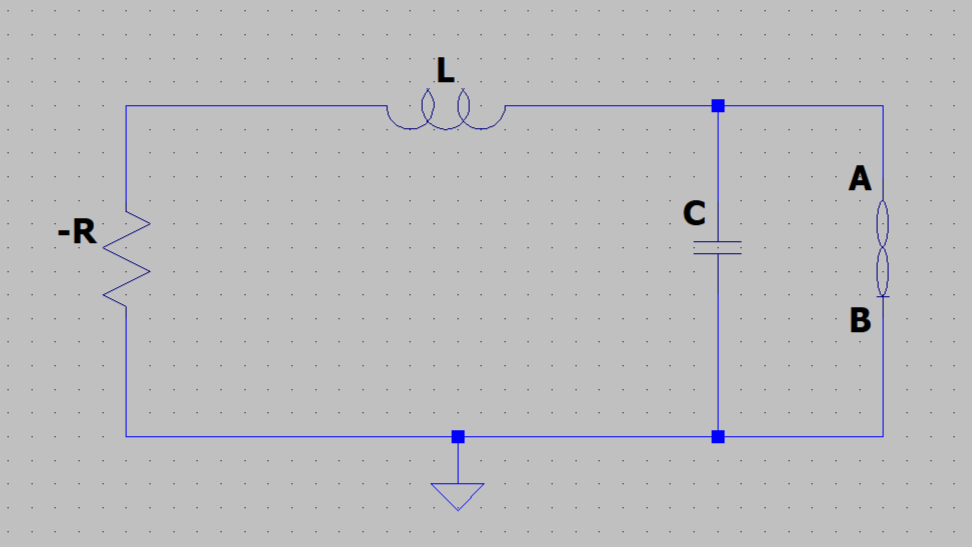
\includegraphics[width=1\textwidth]{-RLCM.png}
		\caption{Oscilador RLC con R negativa y Memristor.}
		\label{fig:-RLCM}
	\end{figure}\smallskip
	
	\vspace{0.5cm}Como se puede ver en la \fref{fig:-RLCM}, no existe una fuente de señal en el circuito, y esto se debe a que el análisis hecho busca encontrar una oscilación periódica tan solo proporcionando condiciones iniciales a la bobina y el condensador, gracias al comportamiento de la resistencia negativa y del memristor. La forma de imponer las condiciones iniciales serían las clásicas, usando fuentes de intensidad en serie y tensión en paralelo con interruptores que se abren en $t=0\:(s)$ para la bobina y el condensador respectivamente.
	
	\newpage
	
	\section{Resistencia negativa}
	
	 Uno de los componentes clave de este circuito es la resistencia negativa, que puede construirse mediante un \textit{Convertidor de Impedancia Negativa (NIC)}. Un NIC es un dispositivo activo, lo que significa que en lugar de disipar energía como lo haría una resistencia convencional, puede suministrar energía a un circuito, como se ilustra en la \fref{fig:NIC}. En términos prácticos, un NIC se utiliza para una variedad de propósitos en circuitos eléctricos o electrónicos, como la compensación de la resistencia de carga de un sistema o  la mejora de la eficiencia en la transferencia de energía. En el contexto de circuitos osciladores, el NIC desempeña un papel crucial al mantener, estabilizar y controlar la frecuencia y calidad de la oscilación.
	 
	\vspace{0.5cm}\begin{figure}[h]
		\centering
		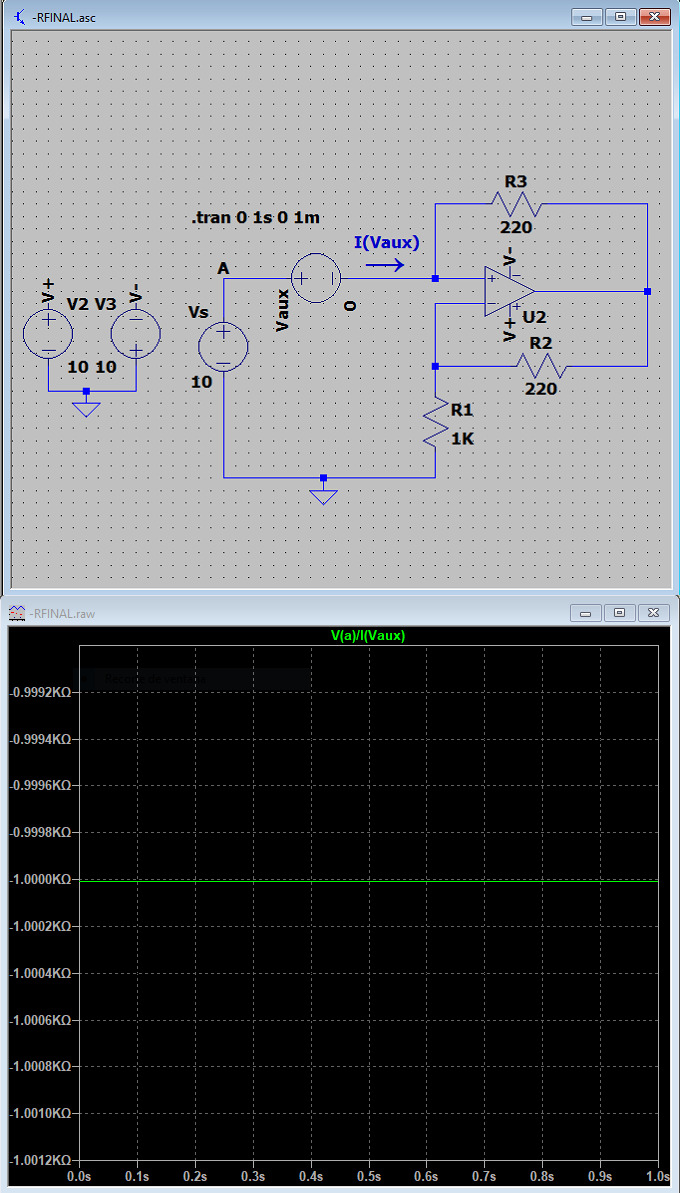
\includegraphics[width=0.65\textwidth]{NIC_B.jpg}
		\caption{Convertidor de Impedancia Negativa de -1000 Ohmios.}
		\label{fig:NIC}
	\end{figure}\smallskip
	
	\newpage
	
	Una de las maneras de realizarlo consiste en utilizar un amplificador operacional y 3 resistencias en la configuración que se ve en la \fref{fig:NIC}. De esta manera si elegimos las resistencias $R_2=R_3$, la resistencia $R_1$ es la que determinaría el valor de resistencia negativa. En efecto:
	
	\vspace{0.5cm}
	
	\begin{center}
	\begin{multicols}{2}
		\centering
		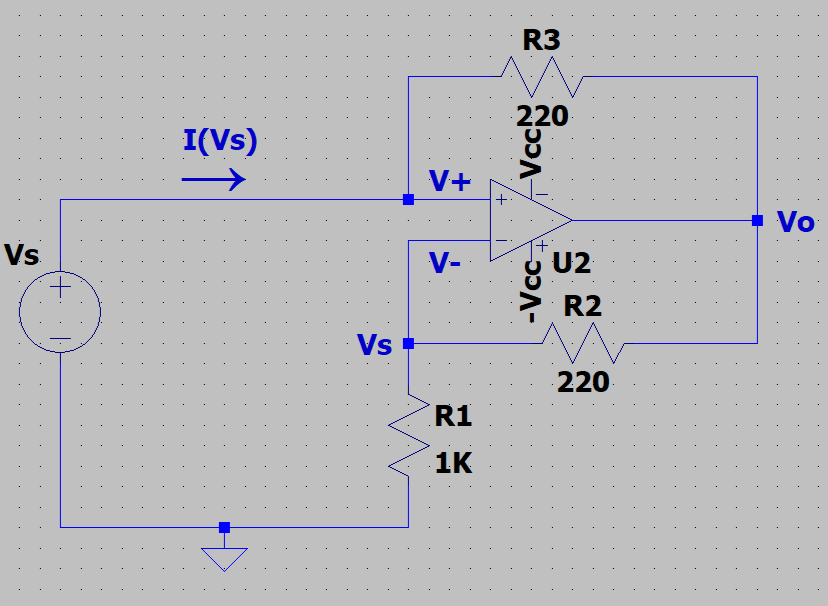
\includegraphics[width=\columnwidth]{demotracion_NIC.png}
		\captionof{figure}{Establecemos los signos de la corriente en el circuito NIC.}
		\label{fig:Param_NIC}
	
		\columnbreak
		
		Consideraciones para el cálculo del circuito de la \fref{fig:Param_NIC} con Amplificadores Operacionales:\\
		\begin{equation}
			V_+\,=\,V_-.
			\label{eq:NIC1}
		\end{equation}
		\begin{equation}
			I_+\,=\,I_-\,=\,0\,(A).
			\label{eq:NIC2}
		\end{equation}
	\end{multicols}
	\end{center}
	
	\noindent Si observamos la ecuación \eref{eq:NIC1}, notamos que la tensión $V_S$ recae sobre la resistencia $R_1$ y se relaciona con la tensión de salida $V_O$ mediante un divisor de tensión:
	
	\begin{equation}
		V_S\,=\,V_O\,\frac{R_1}{R_1 + R_2}\:\Longrightarrow\:V_O\,=\,V_S\,\frac{R_1 + R_2}{R_1}.
		\label{eq:NIC3}
	\end{equation}\smallskip
	
	\noindent Dada la ecuación \eref{eq:NIC2}, la corriente $I(V_S)$ es la misma que fluye a través de la resistencia $R_3$, por lo que podemos deducir:
	
	\begin{equation}
		I(V_S)\,=\,\frac{V_S - V_O}{R_3}.
		\label{eq:NIC4}
	\end{equation}\smallskip
	
	\noindent Sustituyendo la ecuación \eref{eq:NIC3} en \eref{eq:NIC4} y tras directas simplificaciones, llegamos a:
	
	\begin{equation}
		I(V_S)\,=V_S\,\frac{-R_2}{R_1 \, R_3}.
		\label{eq:NIC5}
	\end{equation}\smallskip
	
	\noindent Si dividimos la tensión $V_S$ entre la intensidad $I(V_S)$ (ecuación \eref{eq:NIC5}) para obtener la impedancia de entrada del circuito, obtenemos:
	
	\begin{equation}
		\frac{V_S}{I(V_S)}\,=\,Z_{IN}\,=\,\frac{V_S}{V_S\,\frac{-R_2}{R_1 \, R_3}}\,=\,-R_1\,\frac{R_3}{R_2}.
		\label{eq:NIC6}
	\end{equation}\smallskip
	
	\noindent Si seleccionamos $R_3 = R_2$ en la ecuación \eref{eq:NIC6}, obtendremos:
	
	\begin{equation}
		Z_{IN}\,=\,-R_1.
		\label{eq:NIC7}
	\end{equation}\smallskip
	
	\newpage
	
	\section{Memristor}
	
	 Un componente de gran interés en este circuito es el memristor, cuya teoría fue propuesta por el científico Leon O. Chua en 1971 (ver \cite{chuamissing1971}). Este componente busca resolver un antiguo enigma en las relaciones entre las cuatro variables fundamentales en la teoría de circuitos: voltaje $`` v \textquotedblright$, corriente $`` i \textquotedblright$, carga eléctrica \textit{``q''} y flujo magnético $``\varphi\textquotedblright$. En particular, el memristor establece una relación entre la carga eléctrica y el flujo magnético de la siguiente manera (ver \cite{chuaoscillator2008}):
	
	\begin{equation}
		\varphi\,=\,\varphi(q), \qquad q\,=\,q(\varphi).
		\label{eq:flujocarga}
	\end{equation}\smallskip
	
	\noindent Donde la relación del voltaje y la intensidad respecto a la carga y al flujo en el tiempo es la siguiente:
	
	\begin{equation}
		v(t)\,=\,\frac{d\varphi}{dt}, \qquad i(t)\,=\,\frac{dq}{dt}.
		\label{eq:dvdi}
	\end{equation}
			
	\begin{equation}
		\varphi(t)\,=\,\int_{-\infty}^{t}v(\tau)d\tau, \qquad q(t)\,=\,\int_{-\infty}^{t}i(\tau)d\tau.
		\label{eq:flujocargaintegral}
	\end{equation}\smallskip
	
	\noindent Derivaremos la ecuación \eref{eq:flujocarga} respecto al tiempo, y aplicando la regla de la cadena:
	
	\begin{equation}
		\frac{d\varphi}{dt}\,=\,\frac{d\varphi(q)\,dq}{dq\,dt}, \qquad \frac{dq}{dt}\,=\,\frac{dq(\varphi)\,d\varphi}{d\varphi\,dt}.
		\label{eq:vym}
	\end{equation}\smallskip
	
	\noindent A continuación, sustituyendo las relaciones \eref{eq:dvdi} en \eref{eq:vym} se obtienen las expresiones:
	
	\begin{equation}
		v(t)\,=\,\frac{d\varphi(q)}{dq}i(t), \qquad i(t)\,=\,\frac{dq(\varphi)}{d\varphi}v(t).
		\label{eq:vym2}
	\end{equation}\smallskip
	
	\noindent Las dos relaciones resultantes en \eref{eq:vym2} se conocen como la \textit{Memristancia M(q)} y la \textit{Memductancia W($\varphi$)}:
	
	\begin{equation}
		M(q)\,=\,\frac{d\varphi(q)}{dq}, \qquad W(\varphi)\,=\,\frac{dq(\varphi)}{d\varphi}.
		\label{eq:myw}
	\end{equation}\smallskip
	
	\noindent Por último, se presentan dos expresiones finales que describen el comportamiento del memristor:
	
	\begin{equation}
		\textit{Memristor controlado por carga} \, \Rightarrow \, v(t)\,=\,M(q)\,i(t).
		\label{eq:cc}
	\end{equation}\smallskip
	\begin{equation}
		\textit{Memristor controlado por flujo} \, \Rightarrow \, i(t)\,=\,W(\varphi)\,v(t).
		\label{eq:fc}
	\end{equation}\smallskip
	
	\newpage
	
	 El segundo acontecimiento de notable relevancia en relación al memristor tuvo lugar en el año 2005, cuando los laboratorios de Hewlett-Packard (HP) lograron fabricar un componente cuyo comportamiento exhibía notables similitudes con las características postuladas por Chua para el memristor. Inicialmente, el componente desarrollado por HP había sido denominado como \textit{``Crossbar Latch"}. No obstante, no sería sino hasta 2008 que se percataron de la marcada similitud en su funcionamiento con el concepto original de memristor propuesto por Chua, ver \cite{williams}. La construcción de este componente resulta elegante en su simplicidad, consistiendo en dos capas superpuestas: una compuesta de dióxido de titanio puro y otra de dióxido de titanio con una deficiencia controlada de átomos de oxígeno, ambas encapsuladas entre dos electrodos de platino.
	
\vspace{0.5cm}\begin{figure}[h]
		\centering
		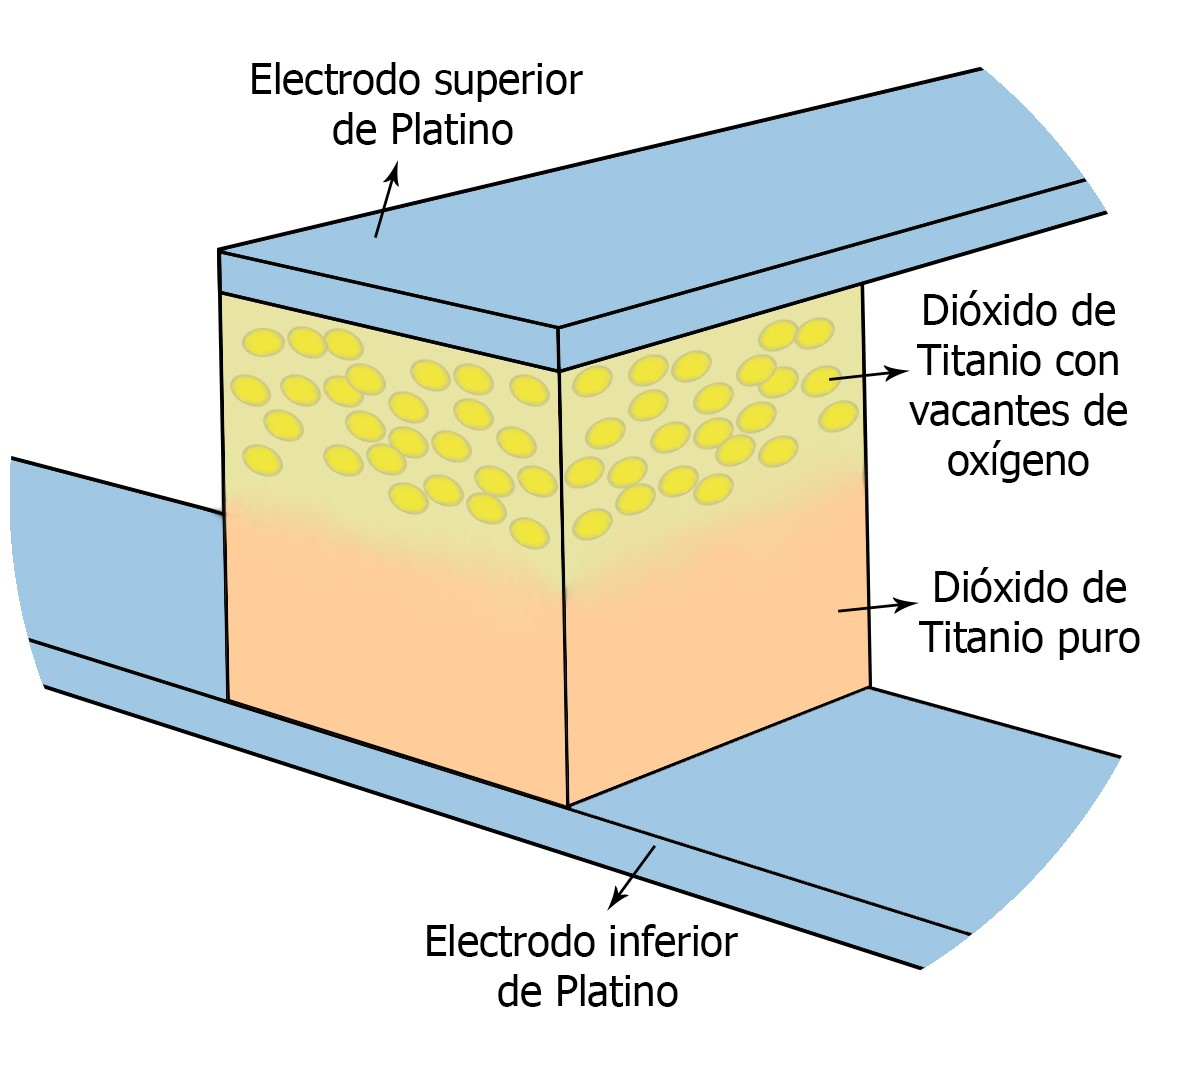
\includegraphics[width=1\textwidth]{mem1.jpg}
		\caption{Costrucción del memristor de HP. Como se propone en \cite{williams}.}
		\label{fig:mem1}
	\end{figure}\smallskip
	
	\newpage
	
	Ahora presentaremos una serie de características del dióxido de titanio que lo convierten en un material altamente atractivo para esta aplicación:
	
	\begin{enumerate}
		\item \textbf{Resistencia variable}: Cuando el dióxido de titanio se dopa, su resistencia eléctrica puede cambiar en respuesta a la aplicación de una corriente o un campo eléctrico. Esto permite no solo almacenar los valores binarios típicos (1 o 0), sino también retener una gama de valores dentro de ciertos límites de operación. Este fenómeno se utiliza en las \textit{Resistive Random-Access Memory (ReRAM)}.
		\item \textbf{No volatilidad}: El dióxido de titanio puede mantener su estado de resistencia incluso cuando se interrumpe la corriente eléctrica que lo atraviesa. Esto significa que puede retener información y mantener su estado de resistencia sin requerir energía continua, lo que es fundamental para la preservación de datos.
		\item \textbf{Cambios rápidos de resistencia}: Esta propiedad permite realizar operaciones de escritura y lectura de datos de manera rápida en el memristor. La velocidad de acceso es crucial para su implementación en aplicaciones de almacenamiento y procesamiento de datos.
		\item \textbf{Baja potencia y tamaño compacto}: El uso eficiente de energía es otro punto fuerte del dióxido de titanio, lo que lo hace adecuado para dispositivos que operan con restricciones de potencia. Además, su tamaño compacto facilita su integración en sistemas electrónicos de diversos tamaños y aplicaciones.
	\end{enumerate}
	
	\vspace{0.5cm}La fórmula propuesta en \cite{HP} para modelar el comportamiento de este dispositivo se expresa mediante las siguientes ecuaciones:
	
	\begin{equation}
		v(t)\,=\,\left(R_{ON}\,\frac{w(t)}{D}+R_{OFF}\left(1-\frac{w(t)}{D}\right)\right)i(t),
		\label{eq:hp1}
	\end{equation}\smallskip
	
	\begin{equation}
		\frac{dw(t)}{dt}\,=\,\mu_V\,\frac{R_{ON}}{D}\,q(t).
		\label{eq:hp2}
	\end{equation}\smallskip
	
	\noindent Integrando la ecuación \eref{eq:hp2} e insertándola en \eref{eq:hp1}, teniendo en cuenta que el valor de resistencia $R_{ON} \ll R_{OFF}$, se obtienen las siguientes expresiones:
	
	\begin{equation}
		w(t)\,=\,\mu_V\,\frac{R_{ON}}{D}\,i(t),
		\label{eq:hp3}
	\end{equation}\smallskip
	
	\begin{equation}
		M(q)\,=\,R_{OFF}\,\left(1-\,\frac{\mu_V\,R_{ON}}{D^2}\,q(t)\right).
		\label{eq:hp4}
	\end{equation}\smallskip
	
	 Las ecuaciones \eref{eq:hp1}-\eref{eq:hp4} describen el comportamiento del memristor de HP y a continuación se muestra el esquema del memristor en la Figura \ref{fig:2021}.
	 
	 \newpage
	
	\vspace{0.5cm}\begin{figure}[h]
		\centering
		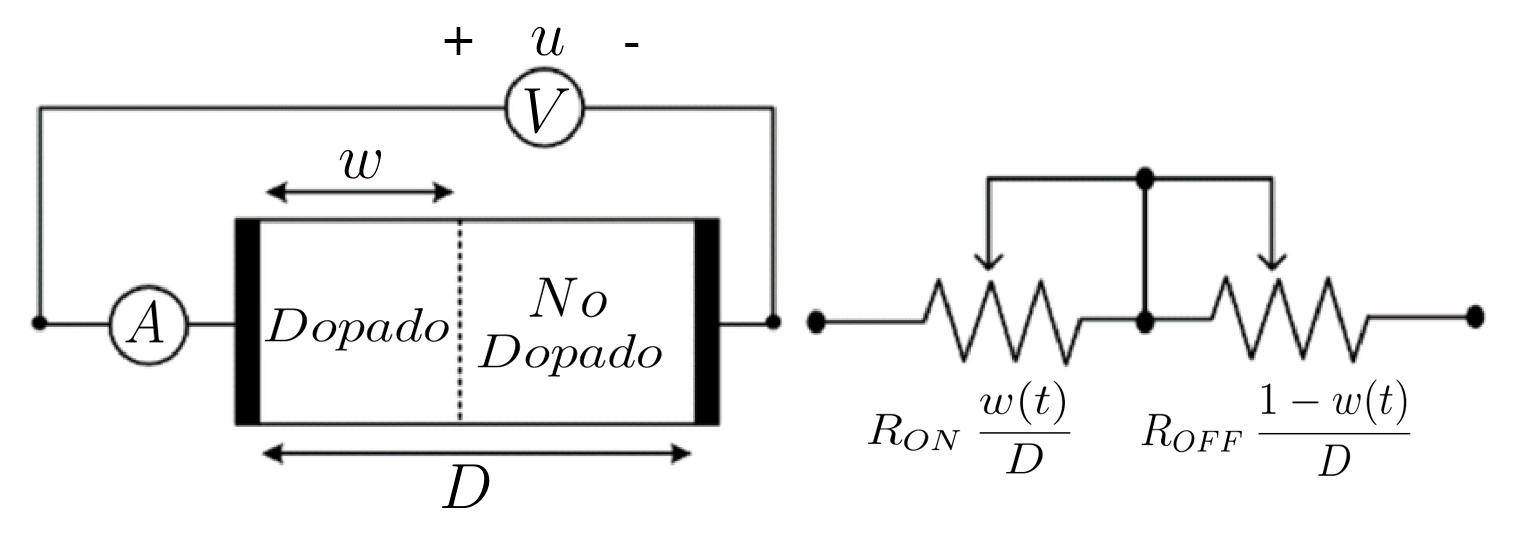
\includegraphics[width=1\textwidth]{schmem.jpg}
		\caption{Esquema del memristor de HP. Propuesto en \cite{2021}.}
		\label{fig:2021}
	\end{figure}\smallskip
	
	 \vspace{0.5cm}Los parámetros que intervienen en las ecuaciones \eref{eq:hp1}-\eref{eq:hp4} y que caracterizan el funcionamiento del componente son:
	
	\begin{enumerate}
		\item $\bm{R_{ON}}$: Resistencia en el estado ON, que representa el valor mínimo de resistencia y es constante.
		\item $\bm{R_{OFF}}$: Resistencia en el estado OFF, que corresponde al valor máximo de resistencia y también es constante.
		\item $\bm{\mu_V}$: Movilidad iónica promedio, una constante que describe la velocidad de movimiento de las partículas iónicas en el dispositivo.
		\item $\bm{w}$: Ancho de la zona dopada, que no es constante y depende de la excitación eléctrica.
		\item $\bm{D}$: Ancho total de la lámina de dióxido de titanio, una constante que define las dimensiones físicas del dispositivo.
	\end{enumerate}\smallskip
	
	El funcionamiento del dispositivo es el siguiente: entre los dos electrodos de platino se encuentra una capa de dióxido de titanio puro $TiO_2$, que actúa como dieléctrico, y otra capa de dióxido de titanio con vacantes de oxígeno $TiO_{2-x}$ que funciona como conductor. Las vacantes de oxígeno están cargadas positivamente, ya que la falta de átomos de oxígeno implica la pérdida de sus electrones de valencia asociados, lo que hace que el compuesto necesite atraer electrones hacia estas vacantes para mantenerse eléctricamente estable (ver \fref{fig:mem1}).
	
	\vspace{0.5cm} Cuando se aplica un voltaje positivo al electrodo superior, las vacantes de oxígeno en la zona dopada son repelidas y se desplazan hacia la región de dióxido de titanio puro, lo que aumenta la conductividad hasta alcanzar el valor de $R_{ON}$. Por otro lado, si se aplica un voltaje negativo, las vacantes de oxígeno se mueven hacia el electrodo superior, disminuyendo la conductividad hasta llegar a $R_{OFF}$.

	 \vspace{0.5cm}A continuación presentaremos una gráfica que muestra la respuesta del memristor ante una señal senoidal con diversas frecuencias. Esta respuesta se obtuvo utilizando un modelo de memristor de SPICE, basado en las ecuaciones de HP \eref{eq:hp1}-\eref{eq:hp4} (consulte \cite{biolek}).
	
	\newpage 
	
		\vspace{0.5cm}\begin{figure}[h]
		\centering
		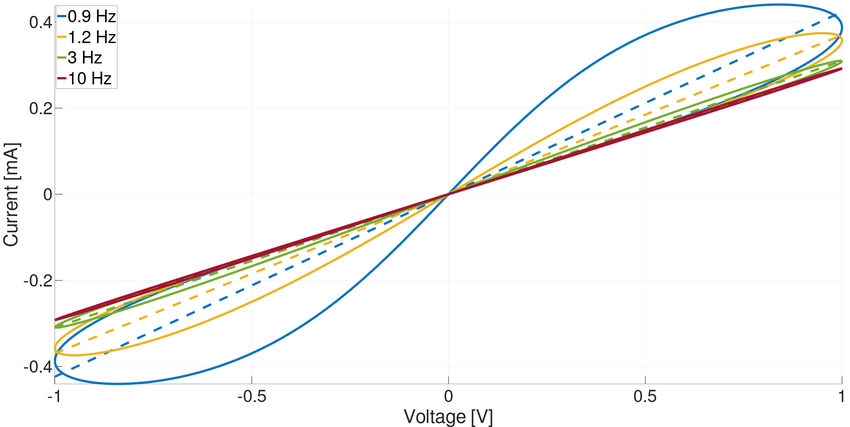
\includegraphics[width=0.9\textwidth]{iv_chua.jpg}
		\caption{Gráfica Tensión-Intensidad del Memristor de Chua ideal para una señal de entrada senoidal con varias frecuencias.}
		\label{fig:iv_chua}
	\end{figure}\smallskip
		
		\vspace{0.5cm} En la \fref{fig:iv_chua} se puede comprobar que a medida que aumenta la frecuencia, la gráfica se asemeja cada vez más a la de una resistencia tradicional, esta característica se puede consultar más en profundidad en \cite{outsiders}.
		
		
	\section{Variables de estado}
	\label{sec:23}
	
	 En este trabajo realizamos un análisis matemático de una bifurcación presente en el circuito oscilador utilizando técnicas de análisis recientes. Sin embargo, antes de adentrarnos en los detalles matemáticos, es fundamental establecer las tensiones e intensidades del circuito (ver \fref{fig:circuito}) y transformar sus ecuaciones eléctricas en una forma matemática que nos permita llevar a cabo un análisis exhaustivo. Comenzaremos nuestro análisis examinando detenidamente el circuito en cuestión.
	
	\vspace{0.5cm}\begin{figure}[h]
		\centering
		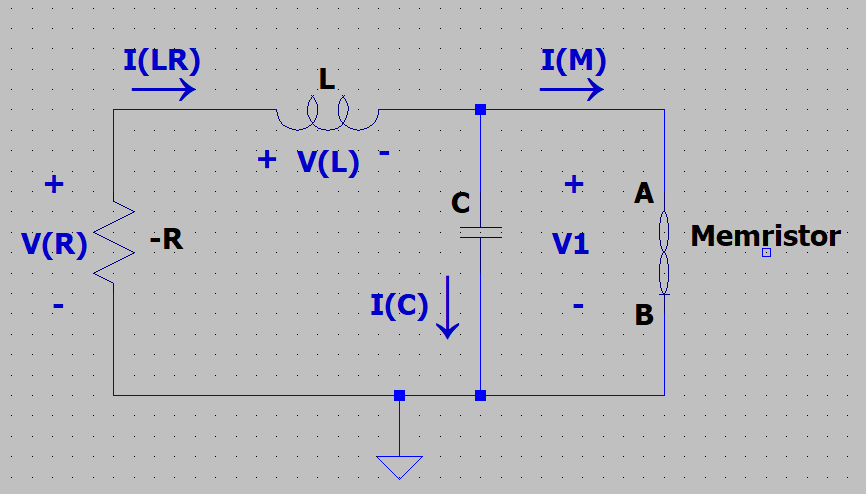
\includegraphics[width=0.9\textwidth]{circuito.png}
		\caption{Magnitudes del circuito.}
		\label{fig:circuito}
	\end{figure}\smallskip
	
	\vspace{0.5cm}\noindent Se aplican las leyes de Kirchoff al circuito de la \fref{fig:circuito} y se obtienen las siguientes ecuaciones:
	\begin{subequations}
		\label{kir}
		\begin{align}
			i_{LR}\,&=\,i_M+i_C, \label{eq:kir1}\\[5mm]
			v_R\,&=\,v_L+v_1.    \label{eq:kir2}
		\end{align}
	\end{subequations}\smallskip
	
	\noindent Reordenando estas ecuaciones, se obtiene:
	\begin{subequations}
		\label{kir2}
		\begin{align}
		i_C\,&=\,i_{LR}-i_M, \label{eq:kir11}\\[5mm]
		v_L\,&=\,v_R-v_1. \label{eq:kir22}
		\end{align}
	\end{subequations}\smallskip
	
	\noindent Teniendo en cuenta la relación entre la carga y el flujo con la intensidad y la tensión de las ecuaciones \eref{eq:dvdi}, así como la ecuación del memristor controlado por flujo \eref{eq:fc}, y aplicándolas a \eref{eq:kir11} y \eref{eq:kir22}, obtenemos el siguiente sistema de ecuaciones diferenciales:
	\begin{subequations}
		\label{kirr}
		\begin{align}
		C\,\frac{dv_1}{dt}\,&=\,i_{LR}-W(\varphi)\,v_1, \label{eq:kir111}\\[2mm]
		L\,\frac{di_{LR}}{dt}\,&=\,R\,i_{LR}-v_1, \label{eq:kir222}\\[2mm]
		\frac{d\varphi}{dt}\,&=\,v_1. \label{eq:kir333}
	\end{align}
	\end{subequations}\smallskip
	
	\newpage
	
	En las ecuaciones \eref{eq:kir111}, \eref{eq:kir222} y \eref{eq:kir333} las variables de estado seleccionadas son la intensidad en la resistencia y la bobina $i_{LR}$, la tensión en el condensador y el memristor $v_1$ y el flujo en el memristor $\varphi$.
	
	\vspace{0.5cm}\noindent Reordenando las ecuaciones anteriores \eref{eq:kir111}, \eref{eq:kir222} y \eref{eq:kir333}, se obtiene el siguiente sistema:
	\begin{subequations}
	\label{siss}
	\begin{align}
		\frac{dv_1}{dt}\,&=\,\frac{i_{LR}}{C}-W(\varphi)\,\frac{v_1}{C} \label{eq:sis1}, \\[2mm]
		\frac{di_{LR}}{dt}\,&=\,\frac{R}{L}\,i_{LR}-\frac{v_1}{L} \label{eq:sis2}, \\[2mm]
		\frac{d\varphi}{dt}\,&=\,v_1. \label{eq:sis3}
	\end{align}
	\end{subequations}\smallskip
	
	\noindent Haciendo algunos cambios a las tres anteriores ecuaciones se llega a construir el siguiente sistema:
    
	\begin{equation}
		\label{eq:sistema1}
		\scalebox{1}{$\displaystyle
			\left\{
			\begin{aligned}
				\frac{dx}{dt} &= \alpha (y - W(z)x), \\
				\frac{dy}{dt} &= -\xi x + \beta y, \\
				\frac{dz}{dt} &= x.
			\end{aligned}
			\right.
			$}
	\end{equation}\smallskip
	
	\noindent Donde tenemos:
	
	\begin{equation*}
		x\,=\,v_1, \qquad y\,=\,i_{LR}, \qquad z\,=\,\varphi, \qquad \alpha\,=\,\frac{1}{C}, \qquad \beta\,=\,\frac{R}{L}, \qquad \xi\,=\,\frac{1}{L}.
	\end{equation*}\smallskip
	
	\noindent El sistema \eref{eq:sistema1} se puede expresar de una forma más general como sigue:
	
	\begin{equation}
		\label{eq:sistema}
			\left\{
			\begin{aligned}
				\frac{dx}{dt} &= a_{11}W(z)x+a_{12}y, \\
				\frac{dy}{dt} &=  a_{21}x+ a_{22}y, \\
				\frac{dz}{dt} &= x.
			\end{aligned}
			\right.
	\end{equation}\smallskip
	
	\noindent Con:
	
	\begin{equation}
		\label{eq:amatriz}
	\begin{gathered}
		a_{11}=-\alpha=-\frac{1}{C}, \qquad a_{12}=\alpha=\frac{1}{C},\\[2mm]
		a_{21}=-\xi =-\frac{1}{L}, \qquad a_{22}=\beta = \frac{R}{L}.
	\end{gathered}
	\end{equation}\smallskip
	
	\newpage
	
	Sin embargo, aún necesitamos definir la función $W(z)$ que aparece en el sistema \eref{eq:sistema}. En \cite{chuaoscillator2008}, se asume que el comportamiento del memristor se puede aproximar mediante una función lineal a trozos monótonamente creciente:
	
	\begin{equation}
		q(\varphi)\,=\,b\varphi+0.5(a-b)(|\varphi+1|-|\varphi-1|).
		\label{eq:qf}
	\end{equation}
    \begin{center}
    	$ donde \quad a,b> 0$
    \end{center}\smallskip
    
    \noindent Derivaremos la expresión \eref{eq:qf} (recordando la ecuación \eref{eq:myw}) para obtener $W(z)$:

   \begin{equation}
    	W(z) = \frac{dq(z)}{dz} =
    	\begin{cases}
    			b,  \quad & z < -1, \\
    			a,  \quad & -1 < z < 1, \\
    			b,  \quad & z > 1.
    	\end{cases}
    	\label{eq:wz}
    \end{equation}\smallskip
	
	\section{Superficies invariantes}
	\label{sec:2.4}
	
	\noindent A continuación, definiremos el concepto de superficie invariante para un sistema dinámico tridimensional. Posteriormente, veremos que el sistema \eref{eq:sistema} posee ciertas superficies invariantes.
	
	\begin{definicion}
		Consideremos el sistema diferencial:
		
		\begin{equation}
			\label{eq:sergio}
			\frac{dX}{dt}=F(X),\qquad X\in \mathbb{R}^3.
		\end{equation}\smallskip
		Se dice que la superficie $S\subset \mathbb{R}^3$ es una superficie invariante para el sistema \eref{eq:sergio} si para cada $X_0 \in S$, la solución del sistema \eref{eq:sergio}, con condición inicial $X(0)=X_0$, pertenece a la superficie $S$ para todo $t$.
	\end{definicion}\smallskip
	
	\vspace{0.5cm} A continuación presentaremos un sistema de ejemplo que posee infinitas esferas invariantes:
	
		\begin{equation}
		\label{eq:ejemesfera}
			\begin{pmatrix}
				\dot{x}\\
				\dot{y}\\
				\dot{z}
			\end{pmatrix} =
			\begin{pmatrix*}[r]
				0 & 3 & -2\\
				-3 & 0 & 1\\
				2 & -1 & 0
			\end{pmatrix*} 
			\begin{pmatrix}
				x\\
				y\\
				z
			\end{pmatrix}
	\end{equation} \smallskip
	
	\vspace{0.5cm}A modo de ejemplo, en la \fref{fig:esfera} hemos representado una esfera invariante del sistema \eref{eq:ejemesfera} con varias órbitas contenida en ella.
	
	\begin{figure}[h]
		\centering
		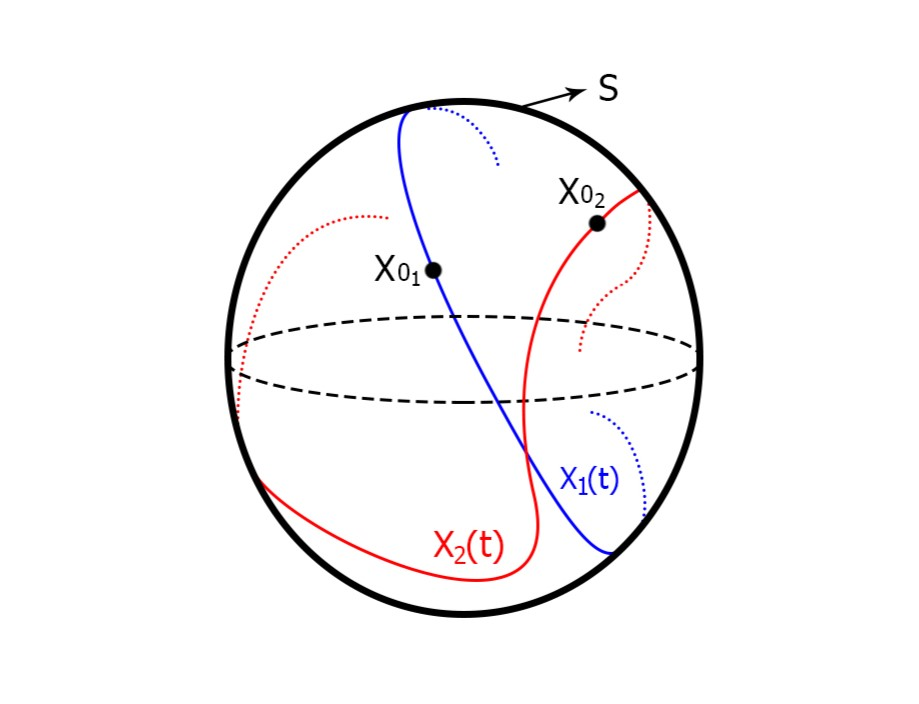
\includegraphics[width=1\textwidth]{esfera.jpg}
		\caption{Esfera con dos órbitas solución $X_1(t)$, $X_2(t)$ con condiciones iniciales $X_1(0)=X_{0_1}$ y $X_2(0)=X_{0_2}$, contenidas en ella.}
		\label{fig:esfera}
	\end{figure}\smallskip
	\newpage
	
	\vspace{0.5cm}Desde el Teorema 1 de \cite{ponce}, sabemos que existe un conjunto de superficies invariantes para el sistema \eref{eq:sistema}. La descripción de estas superficies invariantes se detalla en el siguiente resultado. Se enunciará dicho resultado en este trabajo ya que resultará de especial relevancia.

	\begin{theorem}[Teorema 1 de \cite{ponce}]
		\label{teorema1}
		Consideremos el sistema \eref{eq:sistema} con la función lineal a trozos $q$ dada en \eref{eq:qf} y la función $W(z)$ dada en \eref{eq:wz}. Para cualquier $h \in \mathbb{R}$, el conjunto:
		
		\begin{equation}
			\label{eq:sh}
			S_h=\left\{(x,y,z)\in \mathbb{R}^3\: : \: H(x,y,z)=h \right\},
		\end{equation}
		donde
		\begin{equation}
			\label{eq:hecuation}
			H(x,y,z)=-a_{22}x+a_{12}y-a_{12}a_{21}z+a_{11}a_{22}q(z).
		\end{equation}\smallskip
		
		\noindent es una superficiente invariante para el sistema \eref{eq:sistema}.
		
		\end{theorem}
		
		\vspace{0.5cm}\noindent El sistema \eref{eq:sistema} tiene una familia infinita de superficies invariantes en todo $\mathbb{R}^3$, y la dinámica de los mismos es fundamentalmente bidimensional.
	
	\newpage
	
	\vspace{0.5cm}Como se deduce del Teorema \ref{teorema1} la dinámica del sistema tridimensional \eref{eq:sistema} se puede reducir, aplicando un cambio de variable adecuado, al estudio de un sistema bidimensional. En este trabajo es necesario incluir la prueba de ello porque los cambios de variable nos permitirán obtener la solución periódica en el circuito. Dicha prueba la veremos en el siguiente Teorema con su correspondiente Demostración, pero antes de continuar, definiremos dos matrices auxiliares en el sistema \eref{eq:sistema} teniendo en cuenta la función $W(z)$ \eref{eq:wz}
	
	\begin{equation}
		A_E=\begin{pmatrix*}[c]
			b \, \cdotp a_{11} & a_{12}\\
			a_{21} & a_{22}\\
		\end{pmatrix*}, \qquad 	A_C=\begin{pmatrix*}
			a \, \cdotp a_{11} & a_{12}\\
			a_{21} & a_{22}\\
		\end{pmatrix*}.
	\end{equation}\smallskip
	
	\noindent Con sus correspondientes trazas y determinantes:
	
	\begin{equation}
		\begin{aligned}
			t_E &= b \cdot a_{11} + a_{22},\\
			d_E &= b \cdot a_{11}a_{22} - a_{21}a_{12},\\
			t_C &= a \cdot a_{11} + a_{22},\\
			d_C &= a \cdot a_{11}a_{22} - a_{21}a_{12}.\\
		\end{aligned}
	\end{equation}\smallskip
	
 \vspace{0.5cm}\noindent Los subíndices $E$ y $C$ hacen referencia a las zonas $Externas$ y a la zona $Central$ del sistema trizonal \eref{eq:sis2ec}.
	
	\vspace{0.5cm}
	
	\begin{theorem}[Teorema 2 de \cite{ponce}]
		Consideremos el sistema \eref{eq:sistema}, con la función $W(z)$ dada en \eref{eq:wz}, y supongamos que $a_{22}\neq 0$. La dinámica del sistema \eref{eq:sistema} restringida a cada superficie invariante $S_h$, dada en \eref{eq:sh}, con $h \in \mathbb{R}$, es equivalente a la dinámica del sistema bidimensional:
		
		\begin{equation}
			\label{eq:sis2ec}
			\left\{
			\begin{gathered}
				\dot{\tilde{x}}=F(\tilde{x})-\tilde{y}, \\[2mm]
				\dot{\tilde{y}}=g(\tilde{x})-h,
			\end{gathered}
			\right.
		\end{equation}
		
		donde
		
		\begin{equation}
			\label{eq:f1}
			F(\tilde{x})=
			\left\{
			\begin{aligned}
				&t_E(\tilde{x}-1)+t_C, \quad &si& \quad \tilde{x}>1,\\
				&t_C\tilde{x}, &si& \quad |\tilde{x}|\leq 1,\\
				&t_E(\tilde{x}+1)-t_C, \quad &si& \quad \tilde{x}<-1,
			\end{aligned}
			\right.
		\end{equation}\smallskip
		
		\begin{equation}
			\label{eq:g1}
			g(\tilde{x})=
			\left\{
			\begin{aligned}
				&d_E(\tilde{x}-1)+d_C, \quad &si& \quad \tilde{x}>1,\\
				&d_C\tilde{x}, &si& \quad |\tilde{x}|\leq 1,\\
				&d_E(\tilde{x}+1)-d_C, \quad &si& \quad \tilde{x}<-1.
			\end{aligned}
			\right.
		\end{equation}\smallskip
		
	\end{theorem}
	
	\vspace{0.5cm}
		
	\begin{proof}[\textbf{Demostración}]
		 Cuando $a_{22}\neq0$, desde la ecuación $H(x,y,z)=h$, donde $H$ está dada en \eref{eq:hecuation}, podemos despejar $x$ como:
		
		\begin{equation}
			\label{eq:xeqn}
			x=\frac{a_{12}}{a_{22}}y+a_{11}q(z)-\frac{a_{12}a_{21}}{a_{22}}z-\frac{h}{a_{22}}.
		\end{equation}\smallskip
		
		\noindent Sutituyendo la expresión de $x$ anterior en la segunda y tercera ecuación de \eref{eq:sistema}, conseguimos
		
		\begin{equation}
			\label{eq:cambyz}
			\left\{
			\begin{aligned}
				&\dot{y}=\alpha_1y-\alpha_2z+a_{11}a_{21}q(z)-\frac{a_{21}h}{a_{22}}, \\[2mm]
				&\dot{z}=\alpha_3y-\alpha_4z+a_{11}q(z)-\frac{h}{a_{22}}.
			\end{aligned}
			\right.
		\end{equation}
		
	    \noindent con
		
		\begin{equation}
			\label{eq:alphamatriz}
			\begin{aligned}
				&\alpha_1=\frac{a_{22}^2+a_{12}a_{21}}{a_{22}}, \qquad &\alpha_2=\frac{a_{21}^2a_{12}}{a_{22}},\\[2mm]
				&\alpha_3=\frac{a_{12}}{a_{22}}, \qquad &\alpha_4=\frac{a_{12}a_{21}}{a_{22}}.
			\end{aligned}
		\end{equation}\smallskip
		
		\noindent Seguidamente, considerando el siguiente cambio de variable
		
		\begin{equation}
			\label{eq:xytilde}
			\left\{
			\begin{aligned}
				&\tilde{x}=z, \\[2mm]
				&\tilde{y}=\alpha_1z-\alpha_3y+\frac{h}{a_{22}},
			\end{aligned}
			\right.
		\end{equation}\smallskip
		
		 \noindent el sistema \eref{eq:cambyz} se puede escribir en la forma \eref{eq:sis2ec}, con lo que finaliza la demostración del resultado.
		
	\end{proof}
	
	\vspace{0.5cm}Ahora ofreceremos una breve explicación del significado de los anteriores teoremas. Supongamos que $a_{22}\neq 0$ y tomamos una condición inicial $X_0=(x_0,y_0,z_0)$. Esto fija la superficie invariante $S_{h_0}$ donde está la órbita del sistema con condición inicial $X_0$. Obviamente el valor $h_0$ es $h_0=H(x_0,y_0,z_0)$, con $H$ dada en \eref{eq:hecuation}.
	
	\vspace{0.5cm}A partir del valor $h=h_0$, determinamos la solución $\left( \tilde{x}(t),\tilde{y}(t) \right)$ del sistema \eref{eq:sis2ec} con condición inicial $\tilde{x}(0)=z_0$, $\; \tilde{y}(0)=\alpha_1z_0-\alpha_3y_0+\frac{h_0}{a_{22}}$. La solución $(x(t),y(t),z(t))$ del sistema \eref{eq:sistema} con condición inicial $(x_0,y_0,z_0)$ está dada por:
	
	\begin{equation}
		\label{eq:solsis}
		\scalebox{1}{$\displaystyle
			\left\{
			\begin{aligned}
				z(t)&=\tilde{x}, \\[3mm]
				y(t)&= \frac{\alpha_1\tilde{x}(t)+\frac{h_0}{a_{22}}-\tilde{y}(t)}{\alpha_3},\\[3mm]
				x(t)&=\frac{a_{12}}{a_{22}}\left( \frac{\alpha_1\tilde{x}(t)+\frac{h_0}{a_{22}}-\tilde{y}(t)}{\alpha_3} \right) +a_{11}q(\tilde{x}(t))-\frac{a_{12}a_{21}}{a_{22}}\tilde{x}(t)-\frac{h_0}{a_{22}}.
			\end{aligned}
			\right.
			$}
	\end{equation}\smallskip
	
	\begin{comment}
	\vspace{0.5cm}Una breve explicación del significado de los anteriores teoremas. Supongamos que $a_{22}\neq 0$, si elegimos una condición inicial de nuestro sistema que se encuentre dentro de alguna superficie de las que hemos definido en \eref{eq:sh}, entonces la solución del sistema siempre estará contenida en dicha superficie. Es decir, mirando las ecuaciones \eref{eq:xytilde}; con $\tilde{x}$ calculamos la $z$, con $\tilde{y}$ podemos despejar y calcular la $y$ (recordemos que $h$ ya la hemos definido con las condiciones iniciales), y finalmente con la ecuación \eref{eq:xeqn} calculamos la $x$ .Hemos reducido un sistema tridimensional a uno bidimensional y conocemos el plano a trozos $h$ donde estará contenia la solución del sistema.
	\end{comment}
	
	\begin{comment}
	\vspace{0.5cm}La función $W(z)$ puede ser discontinua, esto dependerá de las carácterísticas del memristor. Aún así esta posible discontinuidad no nos afectará en nuestro trabajo como se demuestra en la sección 3 de \cite{ponce} donde los autores demuestran como pasar en cualquier caso de un modelo discontinuo a un modelo reducido continuo. Además en el artículo de Chua de 2008, ver \cite{chuaoscillator2008} donde se presenta el circuito que estamos estudiando en este trabajo, los autores presentan una aproximación de lo que podrían ser la gráfica flujo-carga del memristor caracterizada por la ecuación \eref{eq:qfz} y la suponen continua.
	\end{comment}
	
	\vspace{0.5cm}Nuestro nuevo sistema de dimensión dos tiene tres zonas como vemos en \eref{eq:sis2ec}, sin embargo en este trabajo nos centraremos en dos de ellas, puesto que buscaremos oscilaciones periódicas bizonales

	
	\chapter{Sistemas Dinámicos Continuos}
	\label{cap.2}
	
	En este capítulo, realizaremos un repaso de los sistemas dinámicos continuos lineales a trozos, ya que hemos reducido nuestro circuito a un sistema de este tipo con las ecuaciones \eref{eq:sistema}. Para hacerlo, primero repasaremos los conceptos fundamentales necesarios, que servirán como base posteriormente.
	
	\section{Sistemas lineales planos}
	\label{sec:sislinplanos}
	
	En esta sección analizaremos los sistemas dinámicos continuos de 2 ecuaciones lineales de primer orden con coeficientes constantes. Algunos de los conceptos y resultados que se reflejan en esta sección pueden verse con más profundidad en \cite{hirsch}, \cite{simmons} y \cite{zill}.
	En primera instancia hay que definir lo que es un sistema dinámico continuo:
	
	\vspace{0.5cm}Un sistema dinámico es un conjunto de ecuaciones de cambio que describen la evolución temporal de algún fenómeno, que puede ser de cualquier naturaleza (eléctrico, económico, cinegético...), de manera que el estado presente del sistema viene determinado por los estados anteriores. El estado del sistema queda descrito por sus variables de estado. Cuando la evolución se estudia considerando el tiempo como una variable  continua, decimos que el sistema es continuo y para analizar este tipo de sistemas la regla determinista que lo gobierna es su sistema de ecuaciones diferenciales.
	
	\vspace{0.5cm} Un sistema de ecuaciones diferenciales lineales con coeficientes constantes en el plano tiene la siguiente forma:
	
	\begin{equation}
		\label{eq:edo2}
		\scalebox{1}{$\displaystyle
			\left\{
			\begin{aligned}
				\dot{x}\,=\,\frac{dx}{dt}\,=\,a_{11}x(t)+a_{12}y(t)+b_1, \\
				\dot{y}\,=\,\frac{dy}{dt}\,=\,a_{21}x(t)+a_{22}y(t)+b_2.
			\end{aligned}
			\right.
			$}
	\end{equation}\smallskip
	
	\noindent Escribiremos el sistema \eref{eq:edo2} en forma matricial:
	
	\begin{equation}
		\label{eq:matrxedo2}
		\scalebox{1}{$\displaystyle
		\begin{pmatrix}
			\dot{x}\\
			\dot{y}\\
		\end{pmatrix} =
		\begin{pmatrix}
			a_{11} & a_{12}\\
		    a_{21} & a_{22}\\
		\end{pmatrix} 
		\begin{pmatrix}
			x\\
			y\\
		\end{pmatrix} + 
		\begin{pmatrix}
			b_1\\
			b_2\\
		\end{pmatrix}
		$}
	\end{equation} \smallskip
	
	\noindent O de forma más simplificada:
	
	\begin{equation}
		\label{eq:sisautonomo}
		\dot{X}\,=\,AX+B.
	\end{equation}\smallskip
	
	\noindent Cuando $B=\vec{0}$ el sistema se denomina homogéneo. Por el contrario cuando $B\neq\vec{0}$ el sistema se denomina no homogéneo. Las condiciones iniciales del sistema serán:
	
	\begin{equation}
		\label{eq:ci}
		\scalebox{1}{$\displaystyle
			\left\{
			\begin{aligned}
				x(0)=x_0, \\
			    y(0)=y_0,
			\end{aligned}
			\right.
			$}
	\end{equation}\smallskip
	
	\noindent Que en forma matricial se escribe como:
	
	\begin{equation}
		\label{cimat}
		X(t_0)=\begin{pmatrix}
			x(0)\\y(0)
		\end{pmatrix}=\begin{pmatrix}
		x_0\\y_0
		\end{pmatrix}=X_0.
	\end{equation}\smallskip
	
	\vspace{0.5cm}\noindent Al conjunto del sistema y a sus condiciones iniciales se le denomina \textit{Problema de Valor Inicial (PVI)}: 
	
	\begin{equation}
	\label{eq:pvi}
	\scalebox{1}{$\displaystyle
		\left\{
		\begin{aligned}
			&\dot{X}=A(t)X+B(t), &\rightarrow& \textit{Sistema Diferencial (S.D.)}\\
			&X(t_0)=X_0. &\rightarrow& \textit{Condiciones Iniciales (C.I.)}
		\end{aligned}
		\right.
		$}
    \end{equation}\smallskip
	
	\vspace{0.5cm} Lo primero que se debe hacer con este tipo de problemas es comprobar la existencia y unicidad de sus soluciones, por ello a continuación presentaremos el Teorema de existencia y unicidad pero se puede consultar mas en profundidad en \cite{perko} y \cite{simmons}.
	
	\begin{theorem}[Existencia y Unicidad]
		\label{thm:interesante}
		Para cada $X_0 \, \in \, \mathbb{R}^2$, el problema de valor inicial \eref{eq:pvi} posee una única solución $X(t)$ definida en todo $\mathbb{R}$.
	\end{theorem}
	\vspace{4mm}
	
	\noindent Una solución
	\begin{equation}
		\label{eq:puntos}
		X(t)=\begin{pmatrix}
			x(t) \\ y(t)
		\end{pmatrix}
	\end{equation}\smallskip
	
	\noindent puede ser considerada como una curva en el plano. Este plano se denomina \textit{Plano de Fases} y las \textit{Curvas Solución} se denomina \textit{Órbitas} o \textit{Trayectorias} del sistema.
	
	
	\vspace{0.5cm}Por último, veamos como obtener y analizar los puntos de equilibrio del sistema lienal plano. Primero escribamos el sistema \eref{eq:edo2} de otra forma para ver los siguientes apartados mejor:
	
	\begin{equation}
		\label{eq:sv}
		\scalebox{1}{$\displaystyle
			\left\{
			\begin{aligned}
				\dot{x}\,=\,\frac{dx}{dt}\,=S(x,y), \\
				\dot{y}\,=\,\frac{dy}{dt}\,=V(x,y).
			\end{aligned}
			\right.
			$}
	\end{equation}\smallskip
	
	\begin{definicion}
		Los puntos $(\overline{x},\overline{y})$ que anulan simultaneamente las funciones $S$ y $V$ del sistema \eref{eq:sv} se denominan Puntos de Equilibrio o Críticos del sistema:
	\end{definicion}

	\begin{eqnarray}
		\label{eq:crit}
			\begin{pmatrix}
				0\\
				0\\
			\end{pmatrix} =
			&\begin{pmatrix}
				a_{11} & a_{12}\\
				a_{21} & a_{22}\\
			\end{pmatrix}&
			\begin{pmatrix}
				\overline{x}\\
				\overline{y}\\
			\end{pmatrix} + 
			\begin{pmatrix}
				b_1\\
				b_2\\
			\end{pmatrix},\nonumber \\[4mm]
			&\begin{pmatrix}
			a_{11} & a_{12}\\
			a_{21} & a_{22}\\
			\end{pmatrix}&
			\begin{pmatrix}
			\overline{x}\\
			\overline{y}\\
			\end{pmatrix} = 
			\begin{pmatrix}
			-b_1\\
			-b_2\\
			\end{pmatrix}, \nonumber \\[4mm]
			&A\,\overline{X}=-b.
	\end{eqnarray}\smallskip
	
	\noindent Si el $\det(A)\neq0$ de \eref{eq:crit}, el sistema posee un único punto de equilibrio; este punto se dice solución constante del sistema.
    
    \begin{comment}
    \vspace{0.5cm}Antes de continuar con el análisis de los puntos de equilibrio debemos conocer que el sistema \eref{eq:sv} se denomina \textit{\textbf{Autónomo}} ya que la variable independiente del tiempo ($\bm{t}$) no aparece de manera explícita en los segundos términos de las ecuaciones.
	\end{comment}
    
    \vspace{0.5cm}\noindent Lo siguiente será realizar una translación del punto de equilibrio para que esté en el origen $(0\; 0)^T$, en caso de no estarlo. Para ello aplicaremos los siguientes cambios de variable:
    
	\begin{equation}
		\label{eq:trans}
		\scalebox{1}{$\displaystyle
			\left\{
			\begin{aligned}
				\tilde{X}=x-\overline{x}, \\
				\tilde{Y}=y-\overline{y}.
			\end{aligned}
			\right.
			$}
	\end{equation}\smallskip
	
\noindent Por lo que ahora tenemos:
	
	\begin{equation}
		\label{eq:trans2}
		\scalebox{1}{$\displaystyle
			\left\{
			\begin{aligned}
				\frac{d\tilde{X}}{dt}\,=S(\tilde{X}-\overline{x},\tilde{Y}-\overline{x}), \\
				\frac{d\tilde{Y}}{dt}\,=V(\tilde{X}-\overline{x},\tilde{Y}-\overline{x}).
			\end{aligned}
			\right.
			$}
	\end{equation}\smallskip
	
	Donde el punto  $(0\; 0)^T$ es el punto de equilibrio.
	
	\vspace{0.5cm}Lo que veremos a continuación es la disposición de las soluciones en torno al punto de equilibrio, y la estabilidiad del mismo. Consideremos el sistema autónomo lineal con punto de equilibrio en el origen que hemos obtenido tras el cambio de variable:
	
	\begin{eqnarray}
		\label{eq:trans3}
			\begin{pmatrix}
				\dot{x}\\
				\dot{y}\\
			\end{pmatrix} =
		   \begin{pmatrix}
				a_{11} & a_{12}\\
				a_{21} & a_{22}\\
			\end{pmatrix}
			\begin{pmatrix}
				x\\
				y\\
			\end{pmatrix}.
	\end{eqnarray} \smallskip
	
	\noindent Como vemos, con el cambio de variable no se ha modificado la matriz $A$ que es la que nos indicará todo respecto a la estabilidad del punto crítico. Veremos los tres casos que se estudian en este trabajo: Foco Asintóticamente Estable, Foco Inestable y Centro. Para una descripción precisa de otros tipos de puntos de equilibrio (nodo, silla, ...) puede consultarse \cite{perko} y \cite{simmons}.
	
	\vspace{0.5cm}\noindent Para conocer la estabilidad de los puntos de equilibrio debemos estudiar el polinomio característico de la matriz $A$:
	
	\begin{equation}
		\label{eq:equilibrio}
		\begin{aligned}
		P_A(\lambda)=&\lambda^2-\tr(A)\lambda+\det(A),\\[1mm]
		&\lambda^2-\tr(A)\lambda+\det(A)=0.\\[7mm]
		\det(A)=& a_{11}a_{22}-a_{12}a_{21},\\[1mm]
		\tr(A) =& a_{11}+a_{22}.\\[7mm]
		\text{Donde los autovalores son}\Longrightarrow& \quad \lambda=\frac{\tr(A)\pm \sqrt{\tr(A)^2-4\,\det(A)}}{2}.
	    \end{aligned}
	\end{equation}
	
	\vspace{0.5cm} A continuación clasificaremos los diferentes tipos de punto de equilibrio dependiendo de los autovalores

	\vspace{1cm}\noindent{\Large\textbullet\quad Foco Asintóticamente Estable}
	
	\vspace{0.3cm}\noindent Las curvas solución tienden al punto de equilibrio en forma espiral. Esta situación se tiene cuando:
	\begin{itemize}
		\item $\tr(A)<0$
		\item $\tr(A)^2-4\, \det(A)<0$
	\end{itemize}
	
	\begin{figure}[h]
		\centering
		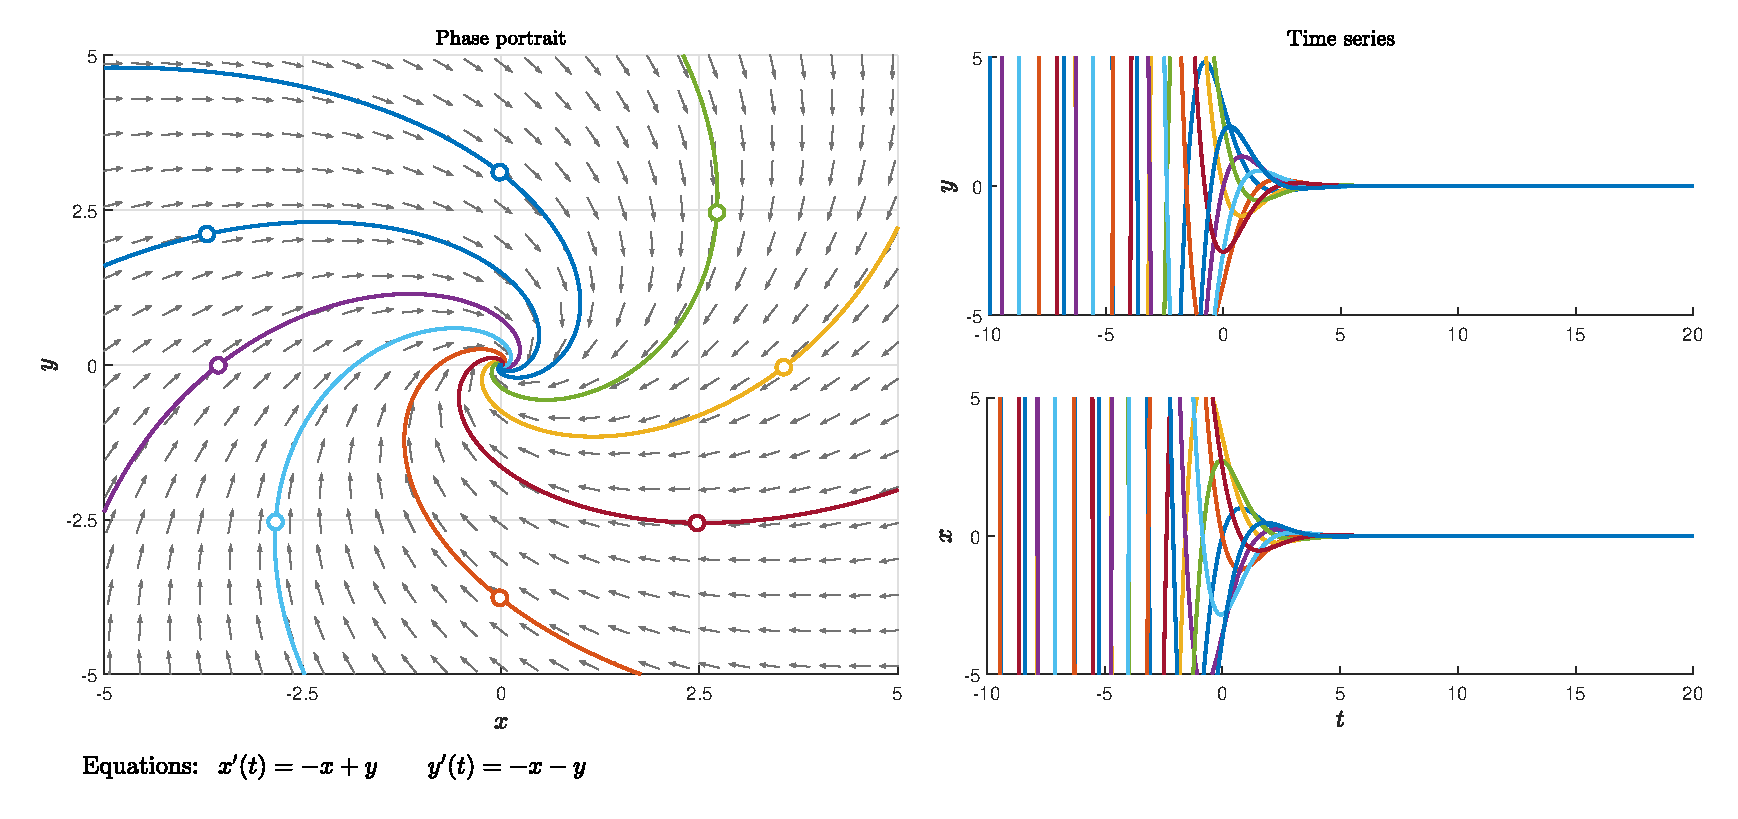
\includegraphics[width=1\textwidth]{estable.eps}
		\caption{Foco asintóticamente estable visto en el plano de fases $xy$ (izquierda) y la variacion de $x$ e $y$ frente al tiempo (derecha).}
		\label{fig:estable}
	\end{figure}\smallskip
	
	\vspace{0.3cm}\noindent Un ejemplo de foco asintóticamente estable se consigue con la matriz:
	
	\begin{equation}
		\label{eq:afe}
		A=\begin{pmatrix*}[r]
			-1 & 1 \\
			-1 & -1
		\end{pmatrix*} \quad \Longrightarrow \quad 
		\left\{ 
		\begin{aligned}
			&\tr(A)=-2<0 \\[2mm]
			&\det(A)=4-4(2)<0
		\end{aligned}
		 \right.
	\end{equation}\smallskip
	
	\noindent En la \fref{fig:estable} podemos observar diferentes órbitas acercándose al foco del sistema \eref{eq:trans3} con la matriz $A$ \eref{eq:afe}. La simulación se ha realizado con la aplicación \textit{Phase Plane and Slope Fields} (ver \cite{phaseplane}), una herramienta diseñada con MATLAB (ver \cite{clevermoller}) para el dibujo en el plano de fases de órbitas de sistemas planos. Esta herramienta se usará a lo alrgo de todo el trabajo.
	
	\newpage
	
	\vspace{1cm}\noindent{\Large\textbullet\quad Foco Inestable}
	
	\vspace{0.3cm}\noindent Las curvas solución tienden al alejarse del punto de equilibrio. Este caso ocurre cuando se cumplen las siguientes condiciones: 
	\begin{itemize}
		\item $\tr(A)>0$
		\item $\tr(A)^2-4\, \det(A)<0$
	\end{itemize}
	
	\begin{figure}[h]
		\centering
		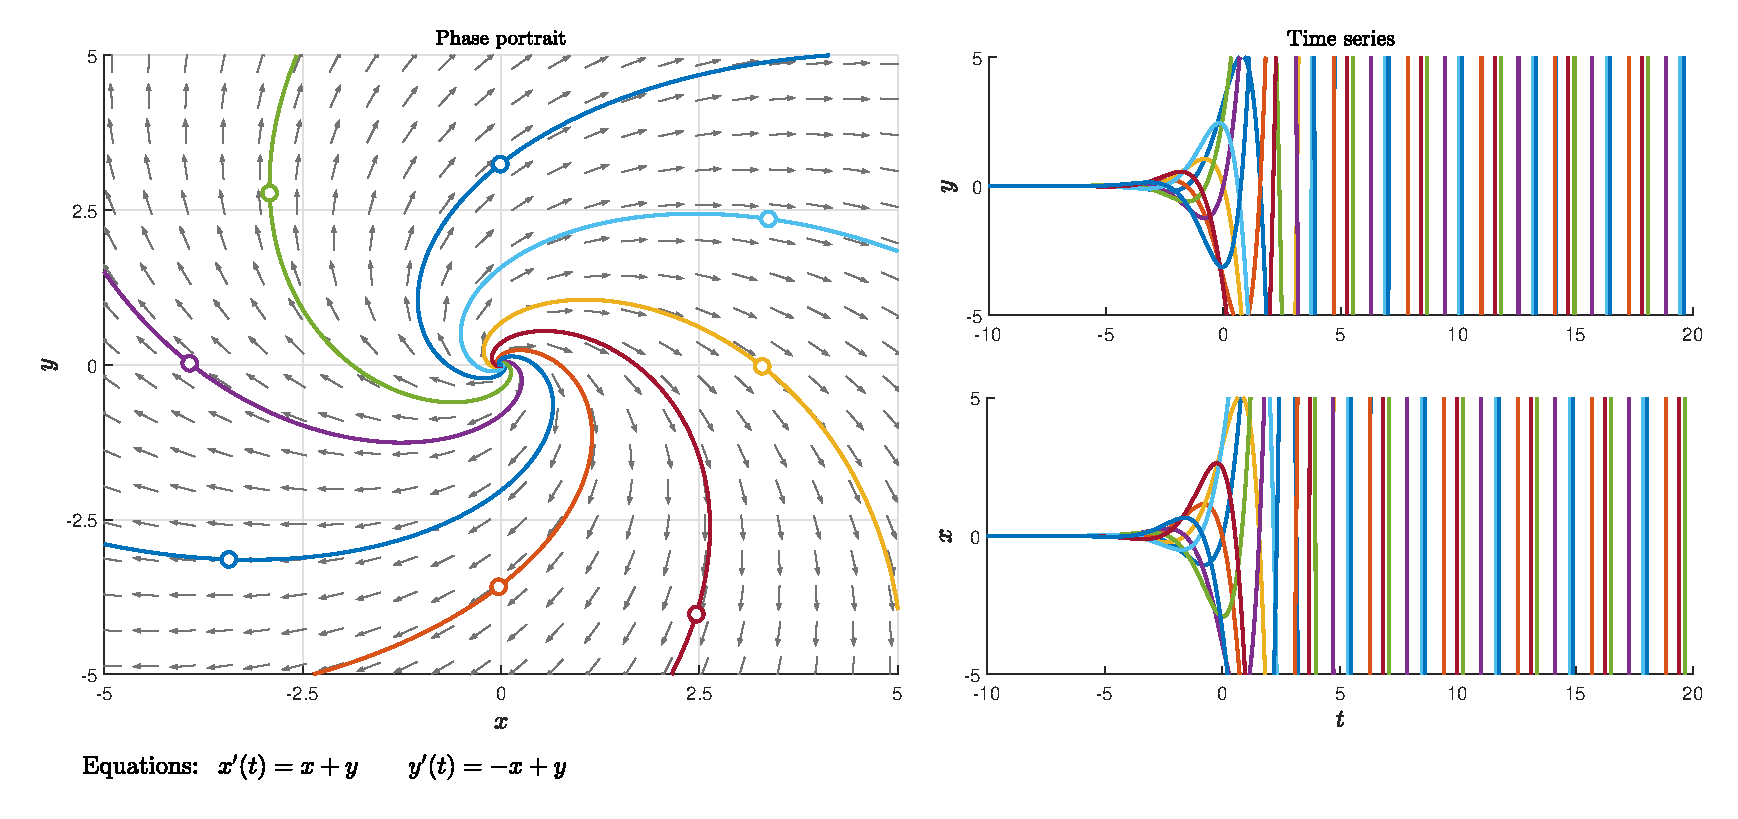
\includegraphics[width=1\textwidth]{inestable.eps}
		\caption{Foco Asintóticamente Inestable visto en el plano de fases $xy$ (izquierda) y la variacion de $x$ e $y$ en el tiempo (derecha).}
		\label{fig:inestable}
	\end{figure}\smallskip
	
	\vspace{0.3cm}\noindent Se puede lograr una situación de foco inestable utilizando la matriz:
	
	\begin{equation}
		\label{eq:afi}
		A=\begin{pmatrix*}[r]
			1 & 1 \\
			-1 & 1
		\end{pmatrix*} \quad \Longrightarrow \quad 
		\left\{ 
		\begin{aligned}
			&\tr(A)=2>0 \\[2mm]
			&\det(A)=4-4(2)<0
		\end{aligned}
		\right.
	\end{equation}\smallskip
	
	\vspace{0.5cm}\noindent En la \fref{fig:inestable}, se pueden notar diversas trayectorias alejándose del punto de equilibrio del sistema \eref{eq:trans3}, empleando la matriz $A$ \eref{eq:afi}.
	
	\newpage
	
    \vspace{1cm}\noindent{\Large\textbullet\quad Centro}
    
    \vspace{0.3cm}\noindent Las curvas solución son concéntricas al punto crítico. Esta circunstancia se presenta cuando se satisfacen las siguientes condiciones: 
    \begin{itemize}
    	\item $\tr(A)=0$
    	\item $\tr(A)^2-4\, \det(A)<0$
    \end{itemize}
    
    \begin{figure}[h]
    	\centering
    	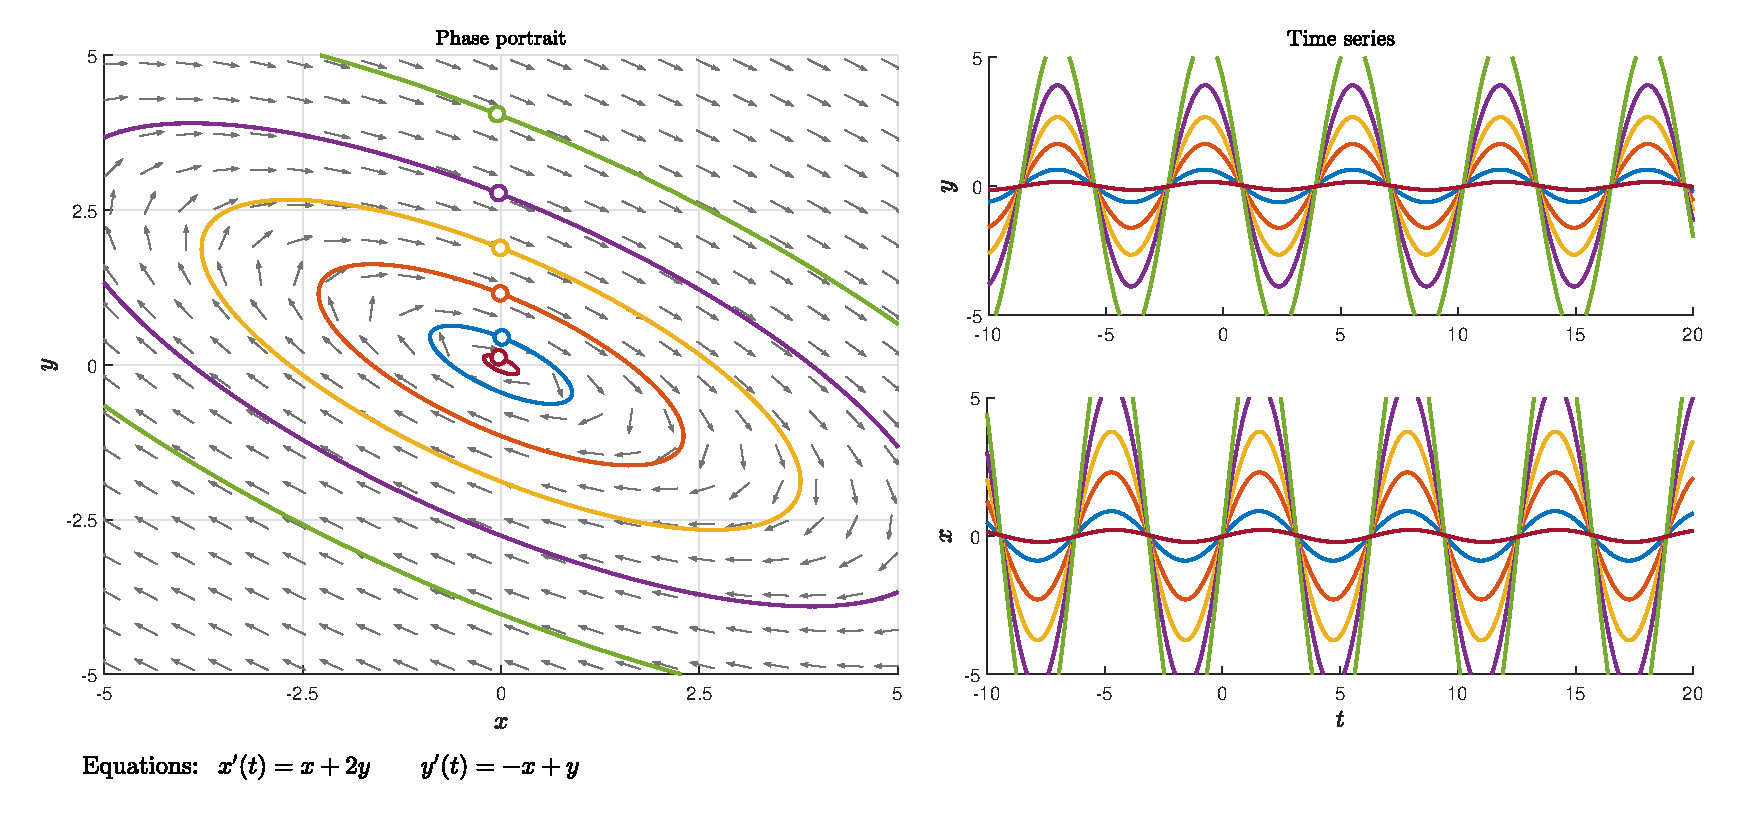
\includegraphics[width=1\textwidth]{centro.eps}
    	\caption{Centro en el plano de fases $xy$ (izquierda) y la variacion de $x$ e $y$ en el tiempo (derecha).}
    	\label{fig:centro}
    \end{figure}\smallskip
    
   	\vspace{0.3cm}\noindent Es posible alcanzar una situación de centro empleando la siguiente matriz:
    
	\begin{equation}
	\label{eq:afc}
	A=\begin{pmatrix*}[r]
		1 & 2 \\
		-1 & -1
	\end{pmatrix*} \quad \Longrightarrow \quad 
	\left\{ 
	\begin{aligned}
		&\tr(A)=1-1=0 \\[2mm]
		&\det(A)=0-4(1)<0
	\end{aligned}
	\right.
\end{equation}\smallskip

\vspace{0.5cm}\noindent En la figura \ref{fig:centro}, se pueden observar múltiples trayectorias concéntricas alrededor del punto de equilibrio del sistema \eref{eq:trans3}, utilizando la matriz $A$ \eref{eq:afc}.
	
	\newpage
	
	\section{Sistemas lineales a trozos bizonales}
	\label{sistrobiz}
	
	 En esta sección, exploraremos el empleo de formas canónicas con el propósito de reducir el conjunto de parámetros que inciden en el sistema, aprovechando estas formas canónicas y las propiedades inherentes a ellas para analizar con mayor profundidad la oscilación periódica en nuestro circuito.
	
	\vspace{0.5cm}\begin{definicion}
		Un sistema dinámico continuo lineal a trozos plano con dos zonas de linealidad es un sistema de ecuaciones diferenciales con la siguiente forma:
	
	\begin{equation}
		\frac{dx}{dt}=\dot{x}=S(x)=
		\label{eq:biz1}
		\scalebox{1}{$\displaystyle
			\left\{
			\begin{aligned}
			 A_1x+b_1\quad si \quad x^T\cdotp w+\delta \leq 0, \\
			 A_2x+b_2\quad si \quad x^T\cdotp w+\delta < 0,
			\end{aligned}
			\right.
			$}
	\end{equation}\smallskip
	
	\noindent donde $x=(x_1,x_2)^T\in \mathbb{R}^2$, las matrices $A_1$ y $A_2$ son reales de orden $2$, $b_1$, $b_2$, $w$ $\in \mathbb{R}^2$ con $w\neq\vec{0}$ y $\delta \in \mathbb{R}$ y se satisface la condición de continuidad: $A_1x+b_1=A_2x+b_2$ sobre la recta de separación:\quad $x^T\cdotp w+\delta = 0.$ 
	
	\end{definicion}
	
	\vspace{0.5cm}\begin{theorem}
		\label{teo:euvic}
		Para cada $X_0 \in \mathbb{R}^2$, el problema de valor inicial asociado al sistema \eref{eq:biz1} con condición inicial $X(0)=X_0$ posee una única solución definida en todo $\mathbb{R}$.
	\end{theorem}
	
	\noindent El Teorema \ref{teo:euvic} y su demostración pueden verse más en profundidad en \cite{docvic}.
	\begin{comment}
	\vspace{0.5cm}\textbf{\textcolor{red}{EXISTENCIA Y UNICIDAD DE SISTEMA 3.14}}

	\noindent Para cada $x^0 \in \mathbb{R}^2$, el problema de valor inicial \eref{eq:pvi2} tiene una solución única $x(t)$ definida para todo $t$ real.
	
	\begin{equation}
		\label{eq:pvi2}
		\scalebox{1.2}{$\displaystyle
			\left\{
			\begin{aligned}
				&\dot{x}=S(x),\\
				&x(0)=x^0.
			\end{aligned}
			\right.
			$}
	\end{equation}\smallskip
	
	 \noindent A continuación veremos la forma canónica más común para los sistemas bizonales que coloca la recta de separación en el eje de ordenadas $x_1=0$.
	\end{comment}
	
	\vspace{0.5cm} Tras un adecuado giro y una conveniente traslación es posible hacer que la recta de separación pueda convertirse en la recta de ecuación $x_1=0$. De esta forma, las matrices del sistema deben compartir sus segundas columnas y los términos independientes de los sistemas a cada lado de la recta $x_1=0$ deben coincidir. Enunciaremos este hecho en el siguiente resultado
	
	\vspace{0.5cm}\begin{proposicion}
		Todo sistema plano lineal a trozos con dos zonas puede escribirse en la forma:
	
	\begin{equation}
		\dot{x}=S(x)=
		\label{eq:lien}
		\scalebox{1}{$\displaystyle
			\left\{
			\begin{aligned}
				B_1x+c\quad si \quad x_1 \leq 0, \\
				B_2x+c\quad si \quad x_1 < 0.
			\end{aligned}
			\right.
			$}
	\end{equation}\smallskip
	
	\noindent donde $x=(x_1,x_2)^T, c\in \mathbb{R}^2$ y las matrices $B_1$, $B_2$ comparten, por continuidad, sus segundas columnas; esto es:
	\begin{equation}
		B_1-B_2 = \left(B_1-B_2\right)e_1e_1^T
	\end{equation}
	
	\noindent siendo $e_1=(1,0)^T$ el primer vector de la base canónica $\mathbb{R}^2$.
    \end{proposicion}\smallskip

\newpage

\begin{comment}
	\noindent La demostración de la anterior definición se lleva a cabo realizando una simetría para que el vector $w$, normal a la recta $x^T\cdotp w+\delta=0$, se transforme en el vector $e_1=(1,0)^T$. Esto se puede hacer usando matrices de Householder, ver \cite{docvic}.
	
	\vspace{0.5cm}\noindent Por último, con una translación hacemos que la nueva recta de separación $x_1=0$ (ahora vertical) pase por el origen. Por lo que el sistema queda con la forma:
	\textbf{\textcolor{red}{y que pasa con $\delta$?}}
	
	\begin{equation}
		\dot{x}=
		\label{eq:lien2}
		\scalebox{1}{$\displaystyle
			\left\{
			\begin{aligned}
			B_1x+c_1\quad si \quad x_1 \leq 0, \\
			B_2x+c_2\quad si \quad x_1 < 0.
			\end{aligned}
			\right.
			$}
	\end{equation}\smallskip
	
	\noindent Con $B_1$ y $B_2$ matrices de orden 2 y $c_1, c_2 \in \mathbb{R}^2$. Nuevamente, por continuidad, se debe satisfacer:
	
	\begin{equation}
		\label{eq:b1b2}
		B_1x+c_1=B_2x+c_2, \qquad si \quad x_1=0.
	\end{equation}\smallskip
	
	\noindent Como el punto $(0,0)^T$ está en la recta de separación $x_1=0$, sustituyéndolo en \eref{eq:b1b2} se tiene que $c_1=c_2$, por lo que:
	
	\begin{equation}
		B_1x=B_2x, \qquad si \quad x_1=0.
	\end{equation}\smallskip
	
	\noindent Como el vector $(0,1)^T$ está sobre la recta de separación $x_1=0$ se tiene por tanto que las dos últimas columnas de $B_1$ y $B_2$ son iguales, sin olvidar que $c_1=c_2=c$.
\end{comment}

	\vspace{0.5cm}Se ha reducido bastante el número de parámetros, ahora tenemos ocho, donde seis de ellos vienen de las matrices $B_1$ y $B_2$ y dos de $c$. Para seguir reduciendo parámetros tengamos en cuenta que estamos buscando oscilaciones que ocupan dos zonas, y estas no aparecen en sistemas unidimensionales, por lo que el primer término de las segundas columnas de las matrices $B_1$ y $B_2$ no puede ser nulo. Esta condición se denomina condición de observabilidad (ver \cite{onsimplyfing} y \cite{docvic}). Mediante el cambio de variable oportuno convertiremos este término en $(-1)$. En primer lugar escribimos el sistema \eref{eq:lien} de la siguiente manera:
	
	\begin{equation}
		\begin{pmatrix*}[r]
			\dot{x}_1 \\ \dot{x}_2
		\end{pmatrix*}=
		\label{eq:lie-1}
		\scalebox{1}{$\displaystyle
			\left\{
			\begin{aligned}
				\begin{pmatrix*}[r]
					b_{11}^1 & b_{12} \\
					b_{21}^1 & b_{22}
				\end{pmatrix*}\begin{pmatrix*}[r]
				x_1\\x_2
				\end{pmatrix*}+\begin{pmatrix*}[r]
				c_1 \\ c_2
				\end{pmatrix*} \quad si \quad x_1 \leq 0, \\
				\begin{pmatrix*}[r]
					b_{11}^2 & b_{12} \\
					b_{21}^2 & b_{22}
				\end{pmatrix*}\begin{pmatrix*}[r]
				x_1\\x_2
				\end{pmatrix*}+\begin{pmatrix*}[r]
					c_1 \\ c_2
				\end{pmatrix*} \quad si \quad x_1 < 0.
			\end{aligned}
			\right.
			$}
	\end{equation}\smallskip
	
	\noindent Aplicamos el siguiente cambio de variable (recordando que $b_{12}\neq0$): 
	
	\begin{equation}
		\label{eq:cambio}
		X_2=-b_{12}\,x_2-c_1,\quad \rightarrow \quad x_2=\frac{-X_2-c_1}{b_{12}}.
	\end{equation}\smallskip

	\noindent Para el caso $x_1\leq 0$ del sistema \eref{eq:lie-1} aplicando el cambio de variable \eref{eq:cambio}:
	
	\begin{equation}
		\label{eq:q1}
	\begin{aligned}
		\dot{x}_1&=b_{11}^1x_1+b_{12}x_2+c-1=b_{11}^1x_1+b_{12}\left(\frac{-X_2-c_1}{b_{12}}\right)+c_1=b_{11}^1x_1-X_2. \\[2mm]
		\dot{X}_2&=-b_{12}\dot{x}_2=-b_{12}\left(b_{21}^1x_1+b_{22}x_2+c_2\right), \\[2mm]
		&=-b_{12}b_{21}^1x_1+b_{22}\left(-b_{12}x_2\right)-b_{12}c_2,  \\[2mm]
		&=-b_{12}b_{21}^1x_1+b_{22}\left(X_2+c_1\right)-b_{12}c_2, \\[2mm]
		&=-b_{12}b_{21}^1x_1+b_{22}X_2+b_{22}c_1-b_{12}c_2.
	\end{aligned}
	\end{equation}\smallskip
	
	\noindent De forma análoga, para $x_1>0$ del sistema \eref{eq:lie-1}:
	
	\begin{equation}
		\label{eq:q2}
		\scalebox{1}{$\displaystyle
			\left\{
			\begin{aligned}
			&\dot{x}_1=b_{11}^2x_1-X_2, \\[2mm]
			&\dot{X}_2=-b_{12}b_{21}^2x_1+b_{22}X_2+b_{22}c_1-b_{12}c_2.
		\end{aligned}
		\right.
		$}
	\end{equation}\smallskip
	
	\noindent Tomando $c_{11}^i=b_{11}^i \: , \: c_{21}^i=-b_{12}b_{21}^i \: , \: c_{22}=b_{22} \: , \: d_2=b_{22}c_1-b_{12}c_2$ y renombrando $X_2$ como $x_2$, obtenemos:
	
	\begin{equation}
		\begin{pmatrix*}[r]
			\dot{x}_1 \\ \dot{x}_2
		\end{pmatrix*}=
		\label{eq:lie-12}
		\scalebox{1}{$\displaystyle
			\left\{
			\begin{aligned}
				\begin{pmatrix*}[r]
					c_{11}^1 & -1 \\
					c_{21}^1 & c_{22}
				\end{pmatrix*}\begin{pmatrix*}[r]
				x_1\\x_2
				\end{pmatrix*}+\begin{pmatrix*}[c]
				0 \\ d_2
				\end{pmatrix*} \quad si \quad x_1 \leq 0, \\
				\begin{pmatrix*}[r]
					c_{11}^2 & -1 \\
					c_{21}^2 & c_{22}
				\end{pmatrix*}\begin{pmatrix*}[r]
				x_1\\x_2
				\end{pmatrix*}+\begin{pmatrix*}[c]
				0 \\ d_2
				\end{pmatrix*} \quad si \quad x_1 < 0.
			\end{aligned}
			\right.
			$} 
	\end{equation}\smallskip
	
	\noindent Se ha conseguido eliminar otros dos parámetros del sistema, además solo se han realizado cambios lineales, por lo que las matrices del sistema son semejantes, es decir, poseen mismos polinomios característicos, autovalores, traza y determinante.
	
	\vspace{0.5cm} Lo que resta es pasar a la forma canónica de Liénard y esto se enuncia en el siguiente resultado.
	

	
	\vspace{0.5cm}\begin{theorem}\label{t2}
		Existe un cambio de variable que transforma el sistema \eref{eq:lie-12} en la forma canónica de Liénard:
	
	\begin{equation}
		\begin{pmatrix*}[r]
			\dot{x}_1 \\ \dot{x}_2
		\end{pmatrix*}=
		\label{eq:lienard}
		\scalebox{1}{$\displaystyle
			\left\{
			\begin{aligned}
				\begin{pmatrix*}[r]
					T_L & -1\\
					D_L & 0
				\end{pmatrix*}\begin{pmatrix*}[r]
				x_1\\x_2
				\end{pmatrix*}-\begin{pmatrix}
				0\\a
				\end{pmatrix} \quad si \quad x_1\leq 0, \\
				\begin{pmatrix*}[r]
					T_R & -1\\
					D_R & 0
				\end{pmatrix*}\begin{pmatrix*}[r]
				x_1\\x_2
				\end{pmatrix*}-\begin{pmatrix}
					0\\a
				\end{pmatrix} \quad si \quad x_1 > 0,
			\end{aligned}
			\right.
			$}
	\end{equation}
	
	\noindent con $a\in \mathbb{R}$.
	\end{theorem}


	\vspace{0.5cm}\begin{proof}[\textbf{Demostración}]
	Usando el siguiente cambio de variable:
	
	\begin{equation}
		\label{eq:cambioo}
		X_2=c_{22}x_1+x_2,\quad \rightarrow \quad x_2=X_2-c_{22}x_1.
	\end{equation}\smallskip
	
	\noindent Para $x_1\leq 0$, el sistema \eref{eq:lie-12} se escribe como:
	
		\begin{equation}
		\label{eq:cambio2}
		\begin{aligned}
			\dot{x}_1&=c_{11}^1x_1-x_2=c_{11}^1x_1-(X_2-c_{22}x_1)=x_1(c_{11}^1+c_{22})-X_2. \\[2mm]
			\dot{X}_2&=c_{22}\dot{x}_1+\dot{x}_2=c_{22}(c_{11}^1x_1-x_2)+(c_{21}^1x_1+c_{22}x_2+d_2), \\[2mm]
			&=c_{22}c_{11}^1x_1-c_{22}x_2+c_{21}^1x_1+c_{22}x_2+d_2, \\[2mm]
			&=x_1(c_{22}c_{11}^1+c_{21})+d_2.
		\end{aligned}
		\end{equation}\smallskip
	
	\noindent De forma análoga, para $x_1>0$ obtenemos:
	
	\begin{equation}
		\label{eq:cambio22}
		\scalebox{1}{$\displaystyle
			\left\{
			\begin{aligned}
				&\dot{x}_1=x_1(c_{11}^2+c_{22})-X_2, \\[2mm]
				&\dot{X}_2=x_1(c_{22}c_{11}^2+c_{21}^2)+d_2.
			\end{aligned}
			\right.
			$}
	\end{equation}\smallskip
	
 	\noindent Tomando $T_L=c_{11}^1+c_{22} \: , \: D_L=c_{22}c_{11}^1+c_{21}^1 \: , \:  T_R=c_{11}^2+c_{22} \: , \: D_R=c_{22}c_{11}^2+c_{21}^2$, renombrando $X_2$ como $x_2$, obtenemos:
	
	\begin{equation}
		\begin{pmatrix*}[r]
			\dot{x}_1 \\ \dot{x}_2
		\end{pmatrix*}=
		\label{eq:lienard2}
		\scalebox{1}{$\displaystyle
			\left\{
			\begin{aligned}
				\begin{pmatrix*}[r]
					T_L & -1\\
					D_L & 0
				\end{pmatrix*}\begin{pmatrix*}[r]
				x_1 \\ x_2
				\end{pmatrix*}+\begin{pmatrix}
					0\\d_2
				\end{pmatrix} \quad si \quad x_1\leq 0, \\
				\begin{pmatrix*}[r]
					T_R & -1\\
					D_R & 0
				\end{pmatrix*}\begin{pmatrix*}[r]
				x_1 \\ x_2
				\end{pmatrix*}+\begin{pmatrix}
					0\\d_2
				\end{pmatrix} \quad si \quad x_1 > 0.
			\end{aligned}
			\right. 
			$}
	\end{equation}\smallskip

	\noindent y tomando $a=-d_2$ terminamos la prueba.
\end{proof}

\vspace{0.5cm}\begin{comentario}
	En el anterior teorema, su correspondiente demostración y a lo largo de lo que resta de trabajo, los términos $T_L,D_L,T_R,D_R$ hacen referencia a las trazas $(T_L,T_R)$ y determinantes $(D_L,D_R)$ de las matrices características de cada uno de los sistemas a la derecha (subíndice $R$) y a la izquierda (subíndice $L$) de la recta de separación.
\end{comentario}\smallskip

	\begin{comment}
	 Por último ajustaremos el parámetro $d_2$. Si $d_2=0$ entonces el sistema ya sería igual que \eref{eq:lienard} pero con el parámetro $a=0$. Si $d_2\neq0$ hay que aplicar el siguiente cambio:
	
	\begin{equation}
		\label{eq:cambiod2}
		X_1=\frac{x_1}{|d_2|}, \qquad X_2=\frac{x_2}{|d_2|}.
	\end{equation}\smallskip
	
	\noindent Por lo que $X_1$ tiene el mismo signo que $x_1$ y la recta de separación sería $X_1=0$.\\[0.5cm]
	Para el caso $X_1\leq 0$ del sistema \eref{eq:lienard2} aplicando el cambio de variable \eref{eq:cambiod2}:
	
	\begin{equation}
		\label{eq:q3}
		\begin{aligned}
			&\dot{X}_1=\frac{\dot{x}_1}{|d_2|}=\frac{tx_1-x_2}{|d_2|}=t\frac{x_1}{|d_2|}-\frac{x_2}{|d_2|}=tX_1-X_2,\\[2mm]
			&\dot{X}_2=\frac{\dot{x}_2}{|d_2|}=\frac{dx_1-0+d_2}{|d_2|}=d\frac{x_1}{|d_2|}+\frac{d_2}{|d_2|}=dX_1+\frac{d_2}{|d_2|}.
		\end{aligned}
	\end{equation}\smallskip
	
	\noindent De forma análoga para $x_1>0$ del sistema \eref{eq:lie-12}:
	
	\begin{equation}
		\label{eq:q4}
		\scalebox{1}{$\displaystyle
			\left\{
			\begin{aligned}
				&\dot{X}_1=TX_1-X_2, \\[2mm]
				&\dot{X}_2=DX_1+\frac{d_2}{|d_2|}.
			\end{aligned}
			\right.
			$}
	\end{equation}\smallskip
	
	\noindent Observemos que cuando dividimos $d_2$ entre su valor absoluto lo que estamos obteniendo es $-1,1,0$ dependiendo de si $d_2$ es negativo, positivo o cero, por lo que usaremos la funcion signo \textit{sgn}:
	
	\begin{equation}
		\label{eq:sgn}
		sgn(d_2)=\left\{
		\begin{aligned}
		1 \qquad si  \quad d_2>0, \\
		0 \qquad si  \quad d_2=0, \\
		-1 \qquad si \quad d_2<0.
    	\end{aligned}
		\right.
	\end{equation}\smallskip
	
	\noindent Sustituyendo \eref{eq:q3} y \eref{eq:q4} en el sistema \eref{eq:lienard2}, tomando $a=-sgn(d_2)$ \textcolor{red}{a=-d2 eso esta bien??} y renombrando $X_1$ como $x_1$ y $X_2$ como $x_2$:
	
	
	\begin{equation}
		\begin{pmatrix*}[r]
			\dot{x}_1 \\ \dot{x}_2
		\end{pmatrix*}=
		\label{eq:lienardfinal}
		\scalebox{1.2}{$\displaystyle
			\left\{
			\begin{aligned}
				\begin{pmatrix*}[r]
					t & -1\\
					d & 0
				\end{pmatrix*}\begin{pmatrix*}[r]
					x_1 \\ x_2
				\end{pmatrix*}-\begin{pmatrix}
					0\\a
				\end{pmatrix} \quad si \quad x_1\leq 0, \\
				\begin{pmatrix*}[r]
					T & -1\\
					D & 0
				\end{pmatrix*}\begin{pmatrix*}[r]
					x_1 \\ x_2
				\end{pmatrix*}-\begin{pmatrix}
					0\\a
				\end{pmatrix} \quad si \quad x_1 > 0.
			\end{aligned}
			\right. 
			$}
	\end{equation}\smallskip
		\end{comment}
	
	\vspace{0.5cm}\noindent Por último, escribiremos el sistema \eref{eq:lienard} de manera más gráfica:
	
	\begin{equation}
		\label{eq:lienardfinalgr}
		\begin{gathered}
			\begin{pmatrix*}[r]
				\dot{x}_1\\ \dot{x}_2
			\end{pmatrix*}= \begin{pmatrix*}[r]
				T_L & -1 \\ D_L & 0
			\end{pmatrix*} \begin{pmatrix*}[r]
				x_1 \\ x_2
			\end{pmatrix*}-\begin{pmatrix*}[c]
				0 \\ a
			\end{pmatrix*} \qquad 
			\rule[-40pt]{1.5pt}{80pt} \qquad 
			\begin{pmatrix*}[r]
				\dot{x}_1\\ \dot{x}_2
			\end{pmatrix*}= \begin{pmatrix*}[r]
				T_R & -1 \\ D_R & 0
			\end{pmatrix*} \begin{pmatrix*}[r]
				x_1 \\ x_2
			\end{pmatrix*}-\begin{pmatrix*}[c]
				0 \\ a
			\end{pmatrix*} \\ x_1=\;0
		\end{gathered}
	\end{equation}\smallskip
	
	\vspace{0.5cm}\noindent Esta forma ``gráfica'' de escribir un sistema lineal a trozos con dos zonas se volverá a usar varias veces a lo largo de esta memoria.
	
	\newpage
	\begin{comment}
	\noindent Las ecuaciones corresponden a las dos zonas izquierda y derecha de la recta de separación $x_1=0$, así que haremos unos cambios de nombre a las variables del sistema \eref{eq:lienardfinal} para que los nombres sean un poco más descriptivos. Finalmente, el sistema en la forma canónica de Liènard nos queda de la siguiente manera:
	
	\begin{equation}
		\begin{pmatrix*}[r]
			\dot{x} \\ \dot{y}
		\end{pmatrix*}=
		\label{eq:lienardrl}
		\scalebox{1.2}{$\displaystyle
			\left\{
			\begin{aligned}
				\begin{pmatrix*}[r]
					T_L & -1\\
					D_L & 0
				\end{pmatrix*}\begin{pmatrix*}[r]
					x \\ y
				\end{pmatrix*}-\begin{pmatrix}
					0\\a
				\end{pmatrix} \quad si \quad x\leq 0, \\
				\begin{pmatrix*}[r]
					T_R & -1\\
					D_R & 0
				\end{pmatrix*}\begin{pmatrix*}[r]
					x \\ y
				\end{pmatrix*}-\begin{pmatrix}
					0\\a
				\end{pmatrix} \quad si \quad x > 0.
			\end{aligned}
			\right. 
			$}
	\end{equation}\smallskip
	
	\vspace{0.5cm}\noindent De una manera más gráfica sería:
	
	\begin{equation}
		\label{eq:lienardrlgr}
		\begin{gathered}
			\begin{pmatrix*}[r]
				\dot{x}\\ \dot{y}
			\end{pmatrix*}= \begin{pmatrix*}[r]
				T_L & -1 \\ D_L & 0
			\end{pmatrix*} \begin{pmatrix*}[r]
				x \\ y
			\end{pmatrix*}-\begin{pmatrix*}[c]
				0 \\ a
			\end{pmatrix*} \qquad 
			\rule[-40pt]{1.5pt}{80pt} \qquad 
			\begin{pmatrix*}[r]
				\dot{x}\\ \dot{y}
			\end{pmatrix*}= \begin{pmatrix*}[r]
				T_R & -1 \\ D_R & 0
			\end{pmatrix*} \begin{pmatrix*}[r]
				x \\ y
			\end{pmatrix*}-\begin{pmatrix*}[c]
				0 \\ a
			\end{pmatrix*} \\ x=\;0
		\end{gathered}
	\end{equation}\smallskip
		\end{comment}

	
	\chapter{Semiaplicaciones de Poincaré}
	\label{sec:4}
	
	Dentro del análisis de sistemas dinámicos, la aplicación de Poincaré emerge como una herramienta de gran utilidad para investigar el comportamiento de un sistema específico. Este enfoque implica la elección de una superficie o una recta (conocida como sección de Poincaré) en el espacio de fases de nuestro sistema, de tal modo que las curva solución de  nuestro sistema atraviesen esta sección, permitiéndonos así examinar el comportamiento de las trayectorias. Cabe destacar que esta aplicación se centra en los puntos de corte de las órbitas con la sección de Poincaré. El análisis de los puntos de corte nos permite obtener información importante sobre el comportamiento dinámico del sistema.
	
	\begin{figure}[h]
		\centering
		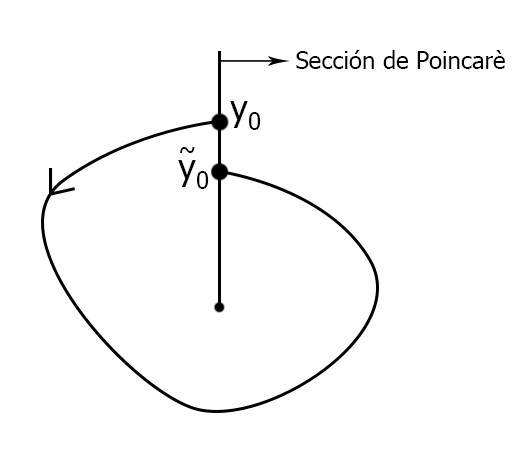
\includegraphics[width=0.8\textwidth]{aplipoincare2.jpg}
		\caption{Punto $y_0$ y su imagen $\tilde{y_0}$ mediante la aplicación de Poincaré. Esta órbita no es periódica}
		\label{fig:aplipoincare2}
	\end{figure}\smallskip

 Como se representa en la \fref{fig:aplipoincare2}, el enfoque de estudio implica una serie de pasos. En primer lugar, se selecciona una sección de Poincaré que corte a la curva solución, posteriormete se elige como punto inicial el punto de corte $y_0$ de dicha curva solución con la sección de Poincaré. Luego, se procede a analizar cómo esta trayectoria evoluciona a lo largo del tiempo y si vuelve a cortar a la sección de Poincaré en un punto $\tilde{y_0}$. En última instancia, si la órbita vuelve a intersectar en el mismo punto, es decir, $y_0=\tilde{y_0}$, podemos concluir que dicha órbita exhibe un comportamiento periódico.

	\newpage
	
	En este trabajo, nos enfocaremos en las semiaplicaciones de Poincarè, lo que significa que examinaremos las dos mitades de la órbita de forma independiente. Este enfoque se justifica en el hecho de que nuestro sistema \eref{eq:lienardfinalgr} es un sistema a trozos, que ya presenta una división en la recta $x_1=0$, la cual se utilizará como sección de Poincaré.
	
	\begin{figure}[h]
		\centering
		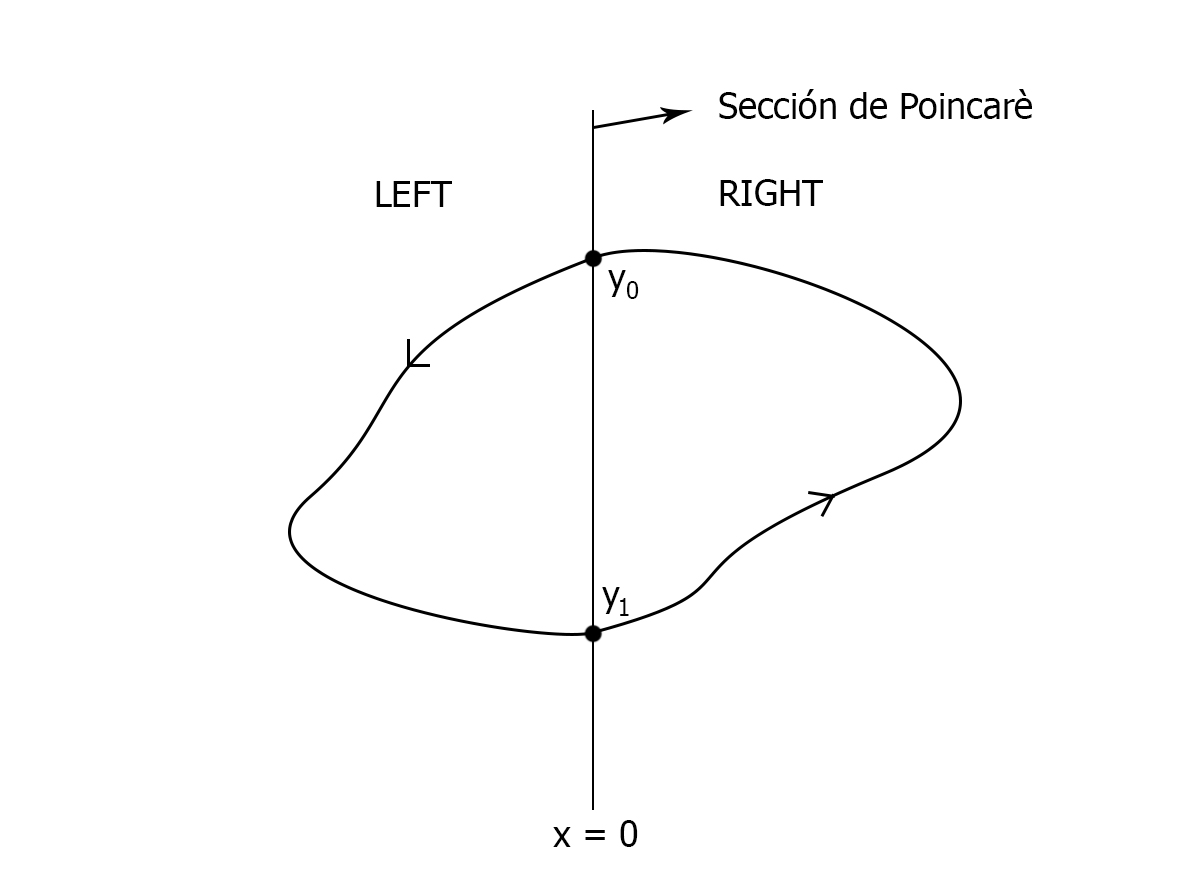
\includegraphics[width=0.9\textwidth]{poincaLR.jpg}
		\caption{Semiaplicaciones de Poincaré derecha e izquierda, las cuales forman una órbita periódica}
		\label{fig:poincaLR}
	\end{figure}\smallskip
	
	En este proceso, identificaremos un punto de intersección inicial, denotado como $y_0$, en la sección de Poincarè. A continuación, procedemos a buscar el siguiente punto de intersección $y_1$ empleando la semiaplicación izquierda. Posteriormente, mediante la semiaplicación derecha, evaluamos si la órbita vuelve a intersectar la sección de Poincarè en el mismo punto $y_0$ (lo que indicaría una órbita periódica, como se ilustra en la \fref{fig:poincaLR}), o si no lo hace (lo que indicaría una órbita no periódica).
	
	\vspace{0.5cm} Puesto que los sistemas que definen el sistema \eref{eq:lienardfinalgr} tienen una misma estructura, definiriemos la semiaplicación de Poincaré izquierda asociada al siguiente sistema lineal para lo que resta de capítulo:
	
		\begin{equation}
		\label{eq:lienardsolo}
		\begin{pmatrix*}[r]
			\dot{x}\\ \dot{y}
		\end{pmatrix*}= \begin{pmatrix*}[r]
			T & -1 \\ D & 0
		\end{pmatrix*} \begin{pmatrix*}[r]
			x \\ y
		\end{pmatrix*}-\begin{pmatrix*}[c]
			0 \\ a
		\end{pmatrix*}.
	\end{equation}\smallskip
	
		\vspace{0.5cm} A continuación presentaremos la definición de la semiaplicación de Poincaré izquierda $P_L$. La definción de la semiaplicación de Poincaré derecha $P_R$ puede hacerse a partir de la semiaplicación izquierda ya que el sistema \eref{eq:lienardsolo} no varia sus propiedades cuando se le aplica el cambio de variable $(x,y,a)\longleftrightarrow(-x,-y,-a)$. 
	
	\newpage
	
	Denotaremos como $\varSigma=\left\{(x,y)^T\in \mathbb{R}^2:x=0\right\}$ a la sección de Poincaré. Nos referiremos con $\varSigma^L$ a la zona izquierda de la sección y $\varSigma^R$ a la zona derecha de la sección (recordemos que los índices $R$ y $L$ harán alusión a las zonas derecha e izquierda). Si evaluamos la primera ecuación de \eref{eq:lienardsolo} en la sección de Poincarè $\varSigma$, tenemos $\dot{x}|_{\varSigma}=-y$, pudiéndose deducir el sentido de las órbitas al atravesar o comenzar en $\varSigma$:
	
	\begin{itemize}
		\item La órbita va de $\varSigma^L$ a $\varSigma^R$ para $y<0$.
		\item La órbita va de $\varSigma^R$ a $\varSigma^L$ para $y>0$.
	\end{itemize}
	
	\vspace{0.5cm}\noindent Asumiremos $a^2+D^2\neq0$, ya que de no ser así, ninguna curva solución cortaría dos veces a $\varSigma$. Esto se puede deducir estudiando la segunda ecuación del sistema \eref{eq:lienardsolo}; para el caso contrario $a=D=0$, tenemos $\dot{y}=Dx+a=0$, y por lo tanto $y$ es constante.
	
	\vspace{0.5cm}\noindent Ahora proporcionaremos la definición rigurosa de la semiaplicación de Poincaré

	\vspace{0.5cm}
	\begin{definicion}
		\label{def6}
		Consideremos el punto $(0,y_0)\in \varSigma$ con $y_0\geq0$, denotaremos por $\phi(t)=(\phi_1(t),\phi_2(t))$ la solución del sistema \eref{eq:lienardsolo}, que para el instante inicial $t=0$ cumple $\phi(0)=(0,y_0)$. Si existe un valor de tiempo $\tau>0$ para el que se cumple $\phi_1(\tau)=0$ y $\phi_1(t)<0$ para todo $t\in(0,\tau)$, decimos que la imagen de $y_0$ mediante la semiaplicación izquierda de Poincaré es $P_L(y_0)=\phi_2(\tau)\leq0$. El valor de tiempo $\tau$ se denomina semitiempo de vuelo izquierdo.
	\end{definicion}
	
	
	\newpage
	
	\vspace{0.5cm} A continuación se puede ver la representación gráfica de las semiaplicaciones izquierda, \fref{fig:semiL}, y derecha, \fref{fig:semiR}, con la nomenclatura adoptada. En \cite{caracterizacion} se puede consultar más en profundidad la definición de la semiaplicación junto con sus dominios de definición.

	
	\begin{figure}[h]
		\centering
		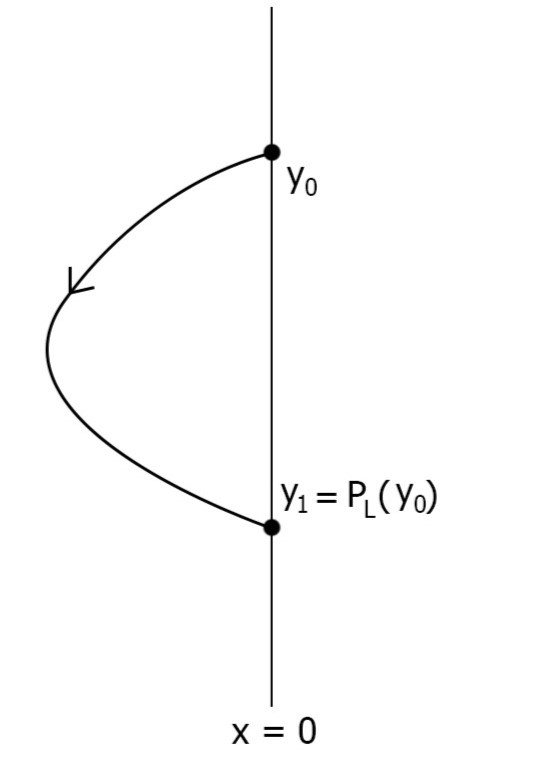
\includegraphics[width=0.55\textwidth]{semiL.jpg}
		\caption{Semiaplicación de Poincaré Izquierda}
		\label{fig:semiL}
	\end{figure}\smallskip
	

	
	\newpage
	
	\begin{figure}[h]
		\centering
		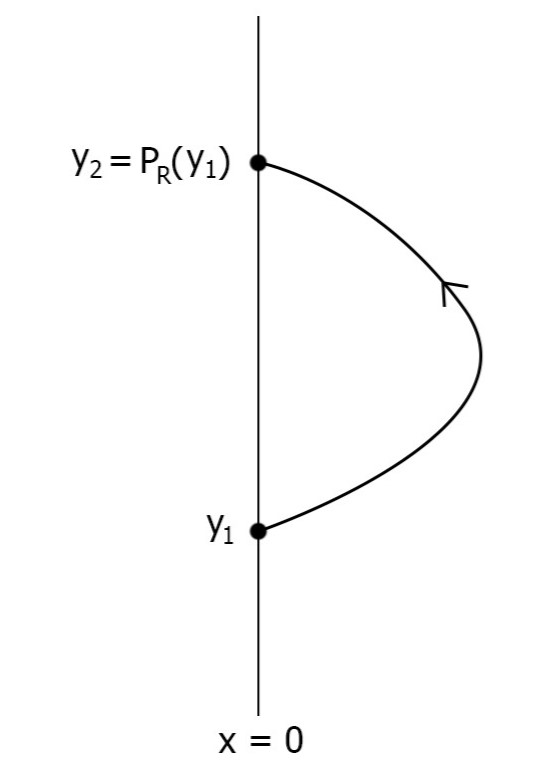
\includegraphics[width=0.55\textwidth]{semiR.jpg}
		\caption{Semiaplicación de Poincaré Derecha}
		\label{fig:semiR}
	\end{figure}\smallskip


	
	\vspace{0.5cm}La Definición \ref{def6} nos invita a abordar la dinámica del sistema a través del cálculo explícito de sus soluciones, un enfoque clásico que conlleva una multiplicidad de casos debido a los espectros (conjunto de autovalores) de las matrices asociadas a cada sistema. Cada uno de estos casos requiere un análisis individual y la aplicación de diversas herramientas matemáticas específicas. Este enfoque puede dar lugar a una complicación considerable en el estudio y conducir a la obtención de resultados aparentemente divergentes para un mismo sistema, dependiendo de la elección de las herramientas matemáticas empleadas en su análisis.
	
	\vspace{0.5cm}\noindent Para evitar esta complejidad, optaremos por la caracterización integral de la semiaplicación de Poincaré, la cual se presenta detalladamente en la siguiente sección y que se encuentra disponible en la referencia \cite{caracterizacion}. Este enfoque nos permitirá abordar el sistema de una manera más coherente y sistemática, evitando las dificultades inherentes a la diversidad de casos que surgen en el enfoque clásico y dejar a un lado, en un principio, el inoportuno semitiempo de vuelo.
	\newpage
	
	\section{Caracterización integral de la semiaplicación de Poincaré}
	
	
	\vspace{0.5cm} Antes de ver las expresiones de la Caracterización Integral se va a presentar el \textit{Valor Principal de Cauchy} ya que se utiliza en las mismas.
	\begin{definicion}
	
	 Consideremos un intervalo $[a,b]$ que contiene al origen y una funcion $f$ continua en $[a,b] \setminus \left\{0\right\}$, el Valor Principal de Cauchy se define como:
	
	\begin{equation}
		\scalebox{1}{$\displaystyle
			PV\left\{\int_{a}^{b}f(x)dx\right\}= \lim_{\epsilon \to 0^+}\left(
			\int_{a}^{-\epsilon}f(x)dx \; + \; 
			\int_{+\epsilon}^{b}f(x)dx
			\right).
			$}
	\end{equation}\smallskip
	
    \end{definicion}
    
	\noindent En \cite{pv} se puede consultar más en profundidad el Valor Principal de Cauchy, así como otras de sus aplicaciones.
	
	\vspace{1cm} A continuación presentaremos las expresiones de la caracterización integral derecha e izquierda, y algunas propiedades de las mismas.
	
	\vspace{1cm}\noindent \textbf{Caracterización integral de la semiaplicación de Poincaré izquierda:}
	
	\vspace{0.5cm} Consideremos el dominio $\mathcal{D}_L$ de la semiaplicación de Poincaré izquierda $P_L$ y un punto $y_0 \in \mathcal{D}_L$
	
	\begin{equation}
		\label{eq:dl}
		\scalebox{1}{$\displaystyle
			\begin{aligned}
				P_L:\mathcal{D}_L\subset [\,0,+\infty) &\longrightarrow ( -\infty,0\, ],\\[2mm]
				y_0 &\longrightarrow y_1.
			\end{aligned}
			$}
	\end{equation}\smallskip
	
	\noindent El valor $y_1$ en el recorrido de $P_L$, $y_1 \in P_L(\mathcal{D}_L)$, es la imagen de $y_0$ mediante $P_L$ si y solo si:
	
	\begin{equation}
		\label{eq:caracl}
		\scalebox{1}{$\displaystyle
			PV\left\{\int_{y_1}^{y_0}\frac{-y}{D_Ly^2-aT_Ly+a^2}dy\right\}=\frac{k_L\pi T_L}{D_L\sqrt{4D_L-T_L^2}}.
			$}
	\end{equation}\smallskip
	
	\noindent donde
	
	\begin{equation*}
		k_L=
		\label{eq:kl}
		\scalebox{1}{$\displaystyle
			\left\{
			\begin{aligned}
				0 \qquad si \quad a>0, \\
				1 \qquad si \quad a=0,\\
				2 \qquad si \quad a<0. 
			\end{aligned}
			\right. 
			$}
	\end{equation*}\smallskip
	
	
		\newpage
	
	\vspace{2cm}\noindent \textbf{Caracterización integral de la semiaplicación de Poincaré derecha:}
	
	\vspace{0.5cm} Consideremos el dominio $\mathcal{D}_R$ de la semiaplicación de Poincaré derecha $P_R$ y un punto $y_0 \in \mathcal{D}_R$
	
	\begin{equation}
		\label{eq:dr}
		\scalebox{1}{$\displaystyle
			\begin{aligned}
				P_R:\mathcal{D}_R\subset (-\infty,0\,] &\longrightarrow [\,0, +\infty),\\[2mm]
				y_1 &\longrightarrow y_2.
			\end{aligned}
			$}
	\end{equation}\smallskip
	
	\noindent El valor $y_1$ en el recorrido de $P_R$, $y_1 \in P_R(\mathcal{D}_R)$, es la imagen de $y_0$ mediante $P_R$ si y solo si:
	
	\vspace{0.5cm}\begin{equation}
		\label{eq:caracr}
		\scalebox{1}{$\displaystyle
			PV\left\{\int_{y_1}^{y_0}\frac{-y}{D_Ry^2-aT_Ry+a^2}dy\right\}=\frac{-k_R\pi T_R}{D_R\sqrt{4D_R-T_R^2}}.
			$}
	\end{equation}\smallskip
	
	\noindent donde
	
	\begin{equation*}
		k_R=
		\label{eq:kr}
		\scalebox{1.2}{$\displaystyle
			\left\{
			\begin{aligned}
				0 \qquad si \quad a<0, \\
				1 \qquad si \quad a=0, \\
				2 \qquad si \quad a>0. 
			\end{aligned}
			\right. 
			$}
	\end{equation*}\smallskip
	
	\vspace{1cm}\noindent En las siguientes páginas, proporcionaremos ejemplos de $P_L$, $P_R$, y $P_R^{-1}$ que dan lugar a una órbita periódica (\fref{fig:aplipoincareLRcerrado}, \fref{fig:aplipoincareL-Rcerrado}) y, por otro lado, ejemplos en los que no se forma una órbita periódica (\fref{fig:aplipoincareLR}, \fref{fig:aplipoincareL-R}).
	
	\newpage
	
	 \begin{figure}[h]
		\centering
		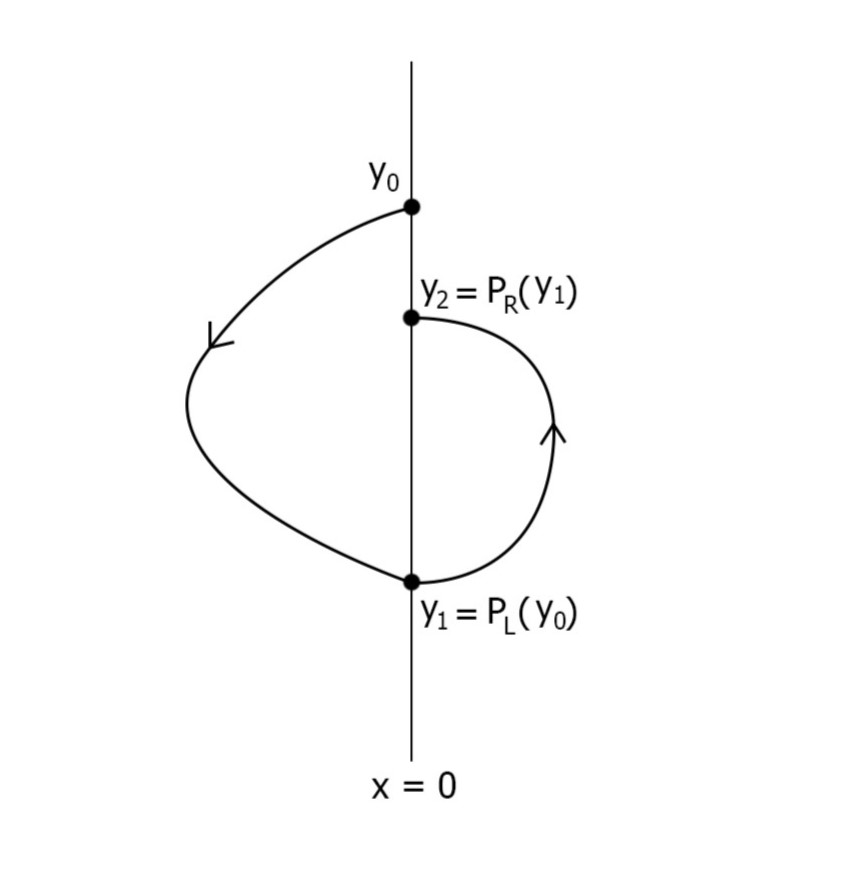
\includegraphics[width=1.1\textwidth,center]{aplipoincareLR.jpg}
		\caption{Semiaplicación izquierda del punto $y_0$ y semiaplicación derecha del punto $y_1$ con diferentes valores $y_0$, $y_2$ por lo que no se ha cerrado la órbita.}
		\label{fig:aplipoincareLR}
	\end{figure}\smallskip
	
	\newpage
	
	\begin{figure}[h]
		\centering
		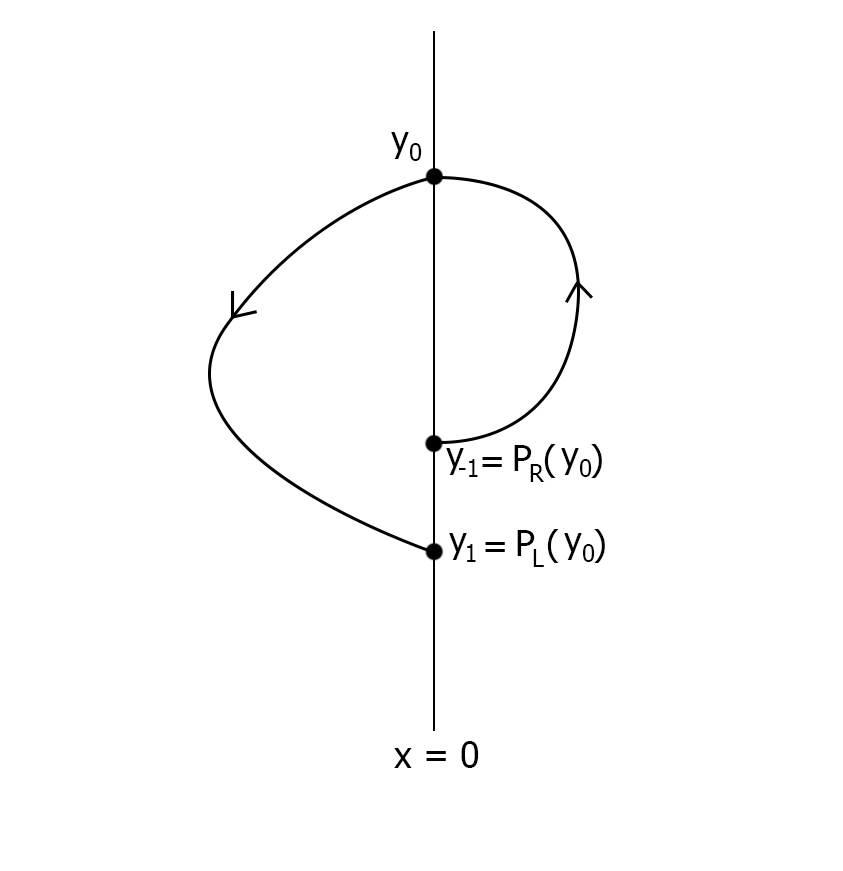
\includegraphics[width=1.1\textwidth,center]{aplipoincareL-R.jpg}
		\caption{Semiaplicación izquierda del punto $y_0$ y la inversa de la semiaplicación derecha del punto $y_0$ con diferentes valores $y_1$, $y_2$ por lo que no se ha cerrado la órbita.}
		\label{fig:aplipoincareL-R}
	\end{figure}
	
	\newpage
	
	\begin{figure}[h]
		\centering
 		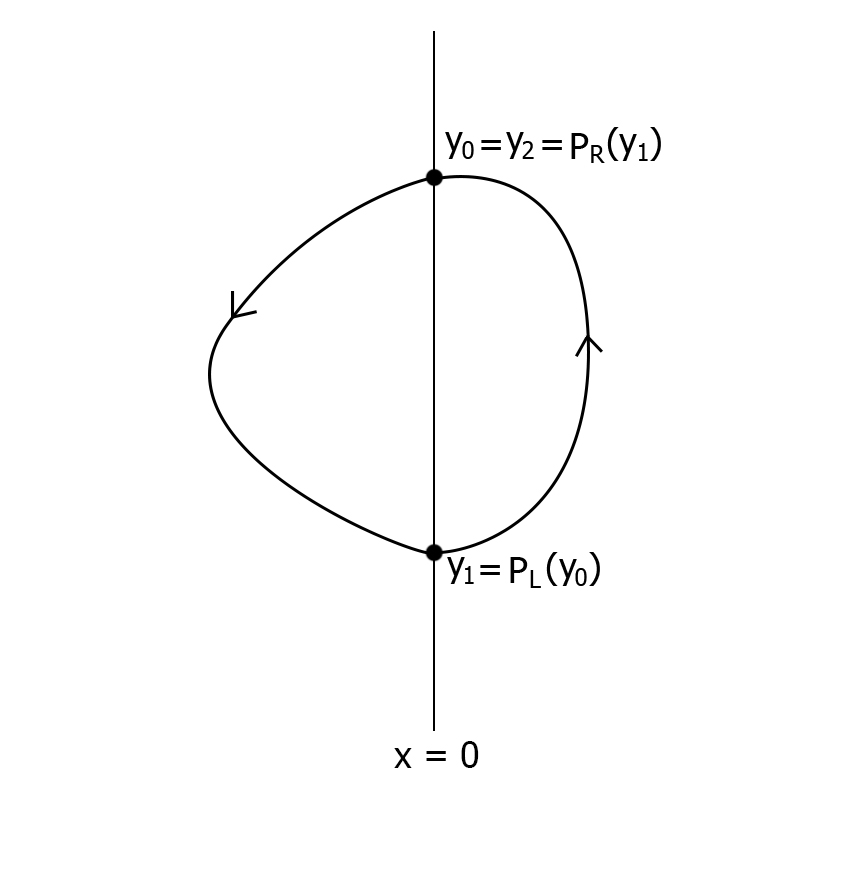
\includegraphics[width=1.1\textwidth,center]{aplipoincareLRcerrado.jpg}
		\caption{Semiaplicación izquierda del punto $y_0$ y semiaplicación derecha del punto $y_1$ con mismos valores $y_0$, $y_2$ por lo que si se ha cerrado la órbita, formándose una órbita periódica.}
		\label{fig:aplipoincareLRcerrado}
	\end{figure}\smallskip
	
	\newpage
	
	\begin{figure}[h]
		\centering
		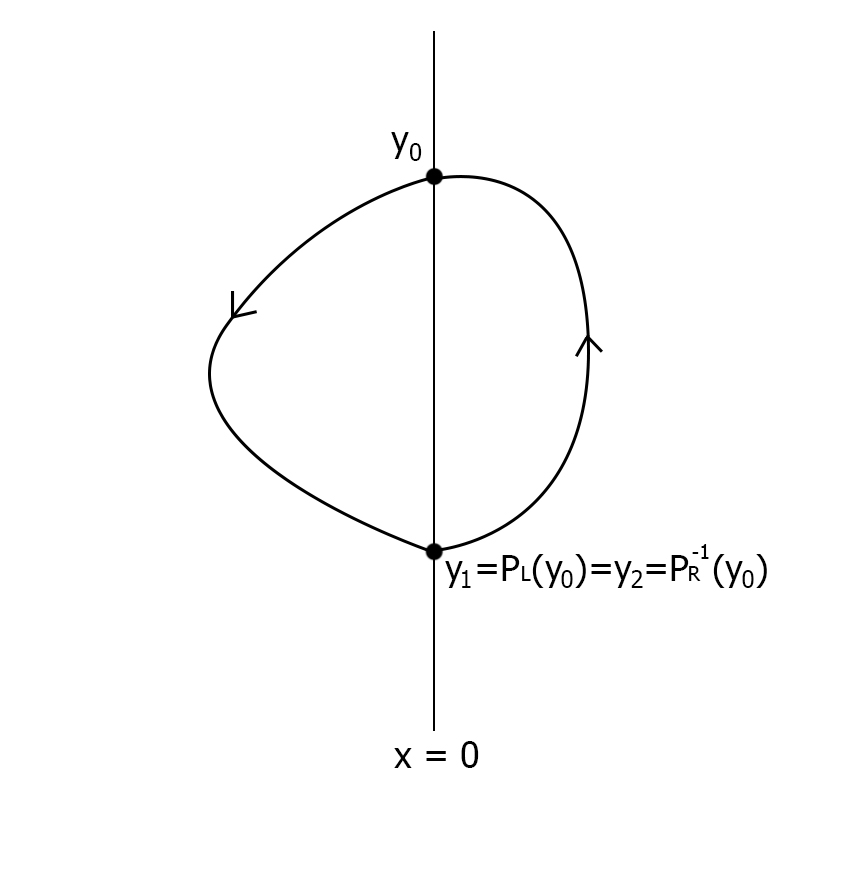
\includegraphics[width=1.1\textwidth,center]{aplipoincareL-Rcerrado.jpg}
		\caption{Semiaplicación izquierda del punto $y_0$ y la inversa de la semiaplicación derecha del punto $y_0$ con mismos valores $y_1$, $y_2$ por lo que si se ha cerrado la órbita formándose una órbita periódica.}
		\label{fig:aplipoincareL-Rcerrado}
	\end{figure}\smallskip
	
	\newpage
	
	\vspace{0.5cm}\noindent Para encontrar una órbita periódica del sistema \eref{eq:lienardfinalgr} debemos buscar valores que cumplan $y_0^*\in \mathcal{D}_L$, $y_1^*\in \mathcal{D}_R$ tales que
	
	\begin{equation*}
		\label{eq:ej1}
		\scalebox{1}{$\displaystyle
			\left\{
			\begin{aligned}
				P_L(y_0^*)=y_1^*, \\
				P_R(y_1^*)=y_0^* ,
			\end{aligned}
			\right. 
			$}
	\end{equation*}\smallskip
	
	\noindent de manera equivalente
	
	\begin{equation*}
		\label{eq:ej2}
		\scalebox{1}{$\displaystyle
			\left\{
			\begin{aligned}
				P_L(y_0^*)=y_1^*, \\
				P_R^{-1}(y_0^*)=y_1^*,
			\end{aligned}
			\right. 
			$}
	\end{equation*}\smallskip
	
	\noindent de modo que
	
	\begin{equation*}
		\scalebox{1}{$\displaystyle
		P_L(y_0^*)=P_R^{-1}(y_0^*),
		$}
	\end{equation*}
	
	\begin{equation*}
		\scalebox{1}{$\displaystyle
		y_0^* \in \mathcal{D}_L \cap P_R(\mathcal{D}_R).
		$}
	\end{equation*}
	
	\vspace{0.5cm}\noindent Recordando que $y_0\geq0$ e $y_1\leq0$, si representamos las gráficas $y_1=P_L(y_0)$ e $y_1=P_R^{-1}(y_0)$, una órbita periódica corresponde a un punto de corte entre dichas gráficas, esto se presenta en la \fref{fig:graficaejemplo}.
	
	\begin{figure}[h]
		\centering
		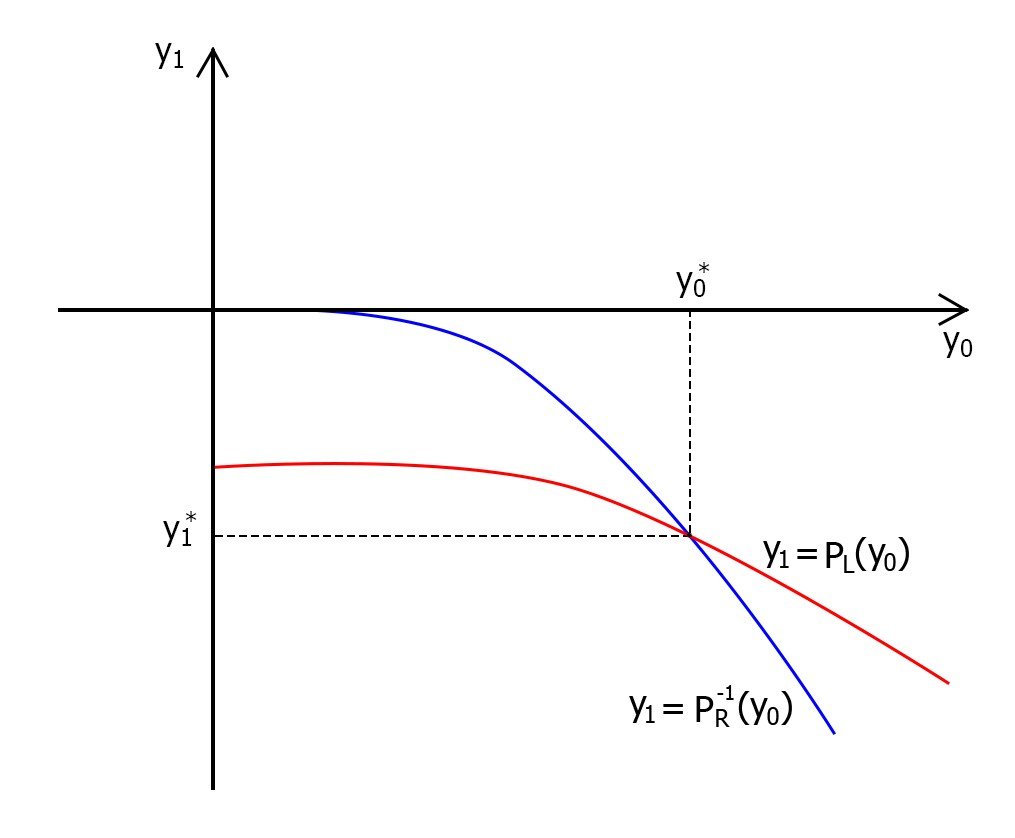
\includegraphics[width=0.8\textwidth]{graficaejemplo.jpg}
		\caption{Punto de corte entre $y_1=P_L(y_0)$ e $y_1=P_R^{-1}(y_0)$ que corresponde a una solución periódica del sistema \eref{eq:lienardfinalgr}}
		\label{fig:graficaejemplo}
	\end{figure}\smallskip
	
	\newpage
	
	\vspace{0.5cm} A continuación veremos un ejemplo de la Caracterización Integral de la semiaplicación de Poincaré en MATLAB para entender un poco mejor la estrategia de busqueda de la órbita periódica.
	
	\vspace{1cm}\lstinputlisting[style=Matlab-editor]{Ejemplo_1.m}
	
	\vspace{1cm}\lstinputlisting[style=Matlab-bw]{cwejem1.m}
	
	\vspace{1cm}\noindent Función usada en ``Ejemplo 1'':
	\vspace{0.5cm}\lstinputlisting[style=Matlab-editor]{semipoinca.m}
	
	\newpage
	
	La función \textit{semipoinca} es la aplicación directa de la caracterización integral en MATLAB. Veamos que se se está haciendo:
	
	\vspace{0.5cm}\noindent Primero vamos a reordenar por ejemplo la expresión de la caracterización izquierda \eref{eq:caracl} (con la expresión de la caracterización derecha el procedimiento es el mismo):
	
	\begin{equation}
			\label{eq:eje1}
		\scalebox{1.2}{$\displaystyle
		\begin{gathered}
			\int_{y_1}^{y_0}\frac{-y}{D_Ly^2-aT_Ly+a^2}dy-\frac{k_L\pi T_L}{D_L\sqrt{4D_L-T_L^2}}=0.
		\end{gathered}
			$}
	\end{equation}\smallskip
	
	\noindent como vemos en \textit{semipoinca} tenemos como argumentos de entrada $k,a,T,D,y_0$ y como argumento de salida $y_1$, por lo que la ecuación \eref{eq:eje1} se puede reducir a:
	
		\begin{equation}
		\label{eq:eje3}
		\scalebox{1.2}{$\displaystyle
				f(y_1)=0.
			$}
	\end{equation}\smallskip
	
	\noindent Finalmente la ecuación \eref{eq:eje3} ya está en la forma adecuada para resolverla con la función \textit{fzero} de MATLAB, introduciendo como punto inicial $-y_0$. La función \textit{fzero} resuelve de manera numérica una ecuación tipo $f(x)=0$ a partir de un punto inicial $x_0$ dado.
	
	\vspace{0.5cm}\noindent El código de ``Ejemplo 1'' describe las características de los sistemas a la izquierda y a la derecha, establece un punto de prueba $y_0=1.5$ y llama a la función \textit{semipoinca} para calcular la semiaplicación de Poincaré izquierda y la inversa de la semiaplicación de Poincaré derecha. Como se ve obtenemos valores diferentes, de hecho, la semiaplicación izquierda tiene un valor mayor que la derecha, gráficamente podría ser perfectamente lo representado en la \fref{fig:aplipoincareL-R}.
	\newpage
	
 	A continuación, procederemos a representar de manera gráfica la semiaplicación izquierda y la inversa de la semiaplicación derecha en un intervalo de puntos $y_0 \in [0, 10]$ para determinar si existe un punto de intersección que nos indique que, para un valor de $y_0$ dado, sus imágenes son idénticas.
	
	\vspace{1cm}\lstinputlisting[style=Matlab-editor]{Ejemplo_2.m}
	
	\vspace{1cm}En este caso, empleamos la función \textit{fplot}, que evalúa la función para diferentes valores de $y_0$, abarcando un rango desde cero hasta diez como hemos definido. La representación gráfica muestra la semiaplicación izquierda en rojo y la semiaplicación inversa derecha en azul (ver \fref{fig:ejem2_2}).
	\newpage
	
	\begin{figure}[h]
		\centering
		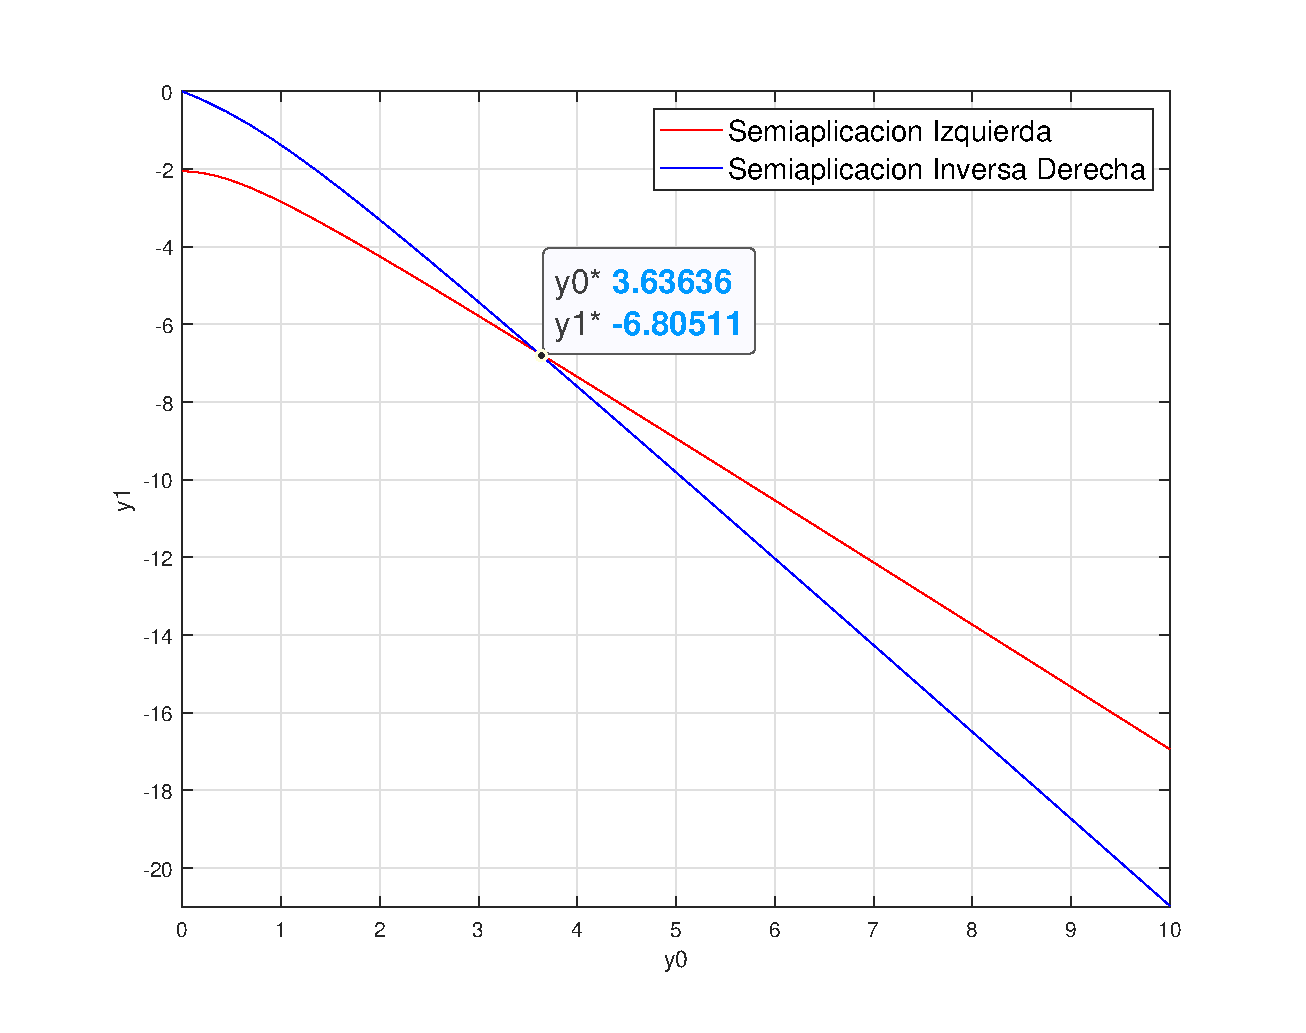
\includegraphics[width=1\textwidth]{g1ejem2.eps}
		\caption{Gráfica obtenida de la semiapliación izquierda y la semiaplicación inversa derecha en el cuarto cuadrante de ``Ejemplo 2''}
		\label{fig:ejem2_2}
	\end{figure}\smallskip
	
	Como vemos en la \fref{fig:ejem2_2} efectivamente se cortan las gráficas, simplemente pinchando más o menos en el punto de corte vemos que las semiaplicación izquierda y la inversa de la semiaplicación derecha tendrán la misma imagen $y_1\approx-6.80511$ cuando $y_0\approx3.63636$.
	\newpage
	
	Una vez hemos identificado un punto cercano a la solución que buscamos, procederemos a calcularla de manera precisa utilizando \textit{fsolve} en MATLAB. Sin embargo, antes de hacerlo, es importante asegurarse de que la función esté escrita de manera correcta.
		
	\vspace{1cm}\lstinputlisting[style=Matlab-editor]{Ejemplo_3.m}
	
	\vspace{1cm}\lstinputlisting[style=Matlab-bw]{cwejem3.m}
	
	\newpage
	
	\noindent Funciones usadas en ``Ejemplo 3'':
	\vspace{0.5cm}\lstinputlisting[style=Matlab-editor]{fsolvepoinca.m}
	\vspace{0.5cm}\lstinputlisting[style=Matlab-editor]{semipoincay1y0.m}
	
	\vspace{1cm} Efectivamente, como se puede apreciar en los resultados de ``Ejemplo 3'', los valores que hemos obtenido son muy similares a los que se observaron en la \fref{fig:ejem2_2}. Por lo tanto, podemos afirmar que, para el sistema que hemos estudiado, existe una solución periódica con $y_0\simeq3.5912$ e $y_1\simeq-6.7065$.

	
	\vspace{0.5cm}Los argumentos de entrada de la función ``fsolvepoinca'' incluyen los parámetros de los sistemas tanto de la derecha como de la izquierda, es decir, $k_L$, $k_R$, $a$, $T_L$, $T_R$, $D_L$ y $D_R$. Además, se utiliza un vector de dos componentes $Y$. Como se puede apreciar en el código de ``Ejemplo 3'', asignamos a este vector el punto de corte que aproximadamente obtuvimos a partir de la gráfica en la \fref{fig:ejem2_2}.
	
	
	\vspace{0.5cm}La función ``fsolve'' en el código de ``Ejemplo 3'' buscará el punto $\left(y_0^*,\: y_1^*\right)$ en el cual las curvas de la semiaplicación izquierda y la semiaplicación inversa derecha se intersecan.
	\newpage
	Por último, para confirmar la validez de nuestro análisis, realizaremos una simulación. Para ello, debemos reformular las ecuaciones de manera que puedan ser implementadas en la aplicación Phase Plane de MATLAB que ya se ha utilizado anteriormente en este trabajo. Tenemos el sistema lineal a trozos \eref{eq:lienardfinalgr}, que podemos expresar de la siguiente manera utilizando valores absolutos. También podríamos haber utilizado la función de MATLAB que define funciones a trozos, la función ``signo'' o las funciones \textit{mkpp} y \textit{ppval}.
	
	\begin{equation}
		\label{eq:clejem}
		\scalebox{1}{$\displaystyle
			\left\{
			\begin{aligned}
			\dot{x}&=\frac{1}{2}\left( x\left(T_R+T_L\right)+\mid x\mid \left(T_R-T_L\right)\right)-y,
				 \\[2mm]
			\dot{y}&=\frac{1}{2}\left( x\left(D_R+D_L\right)+\mid x\mid \left(D_R-D_L\right)\right)-a,
			\end{aligned}
			\right. 
			$}
	\end{equation}\smallskip
	\begin{equation*}
		T_L=0.3, \qquad T_R=-0.5, \qquad D_L=D_R=1, \qquad a=-1.
	\end{equation*}\smallskip
	
	\begin{figure}[h]
		\centering
		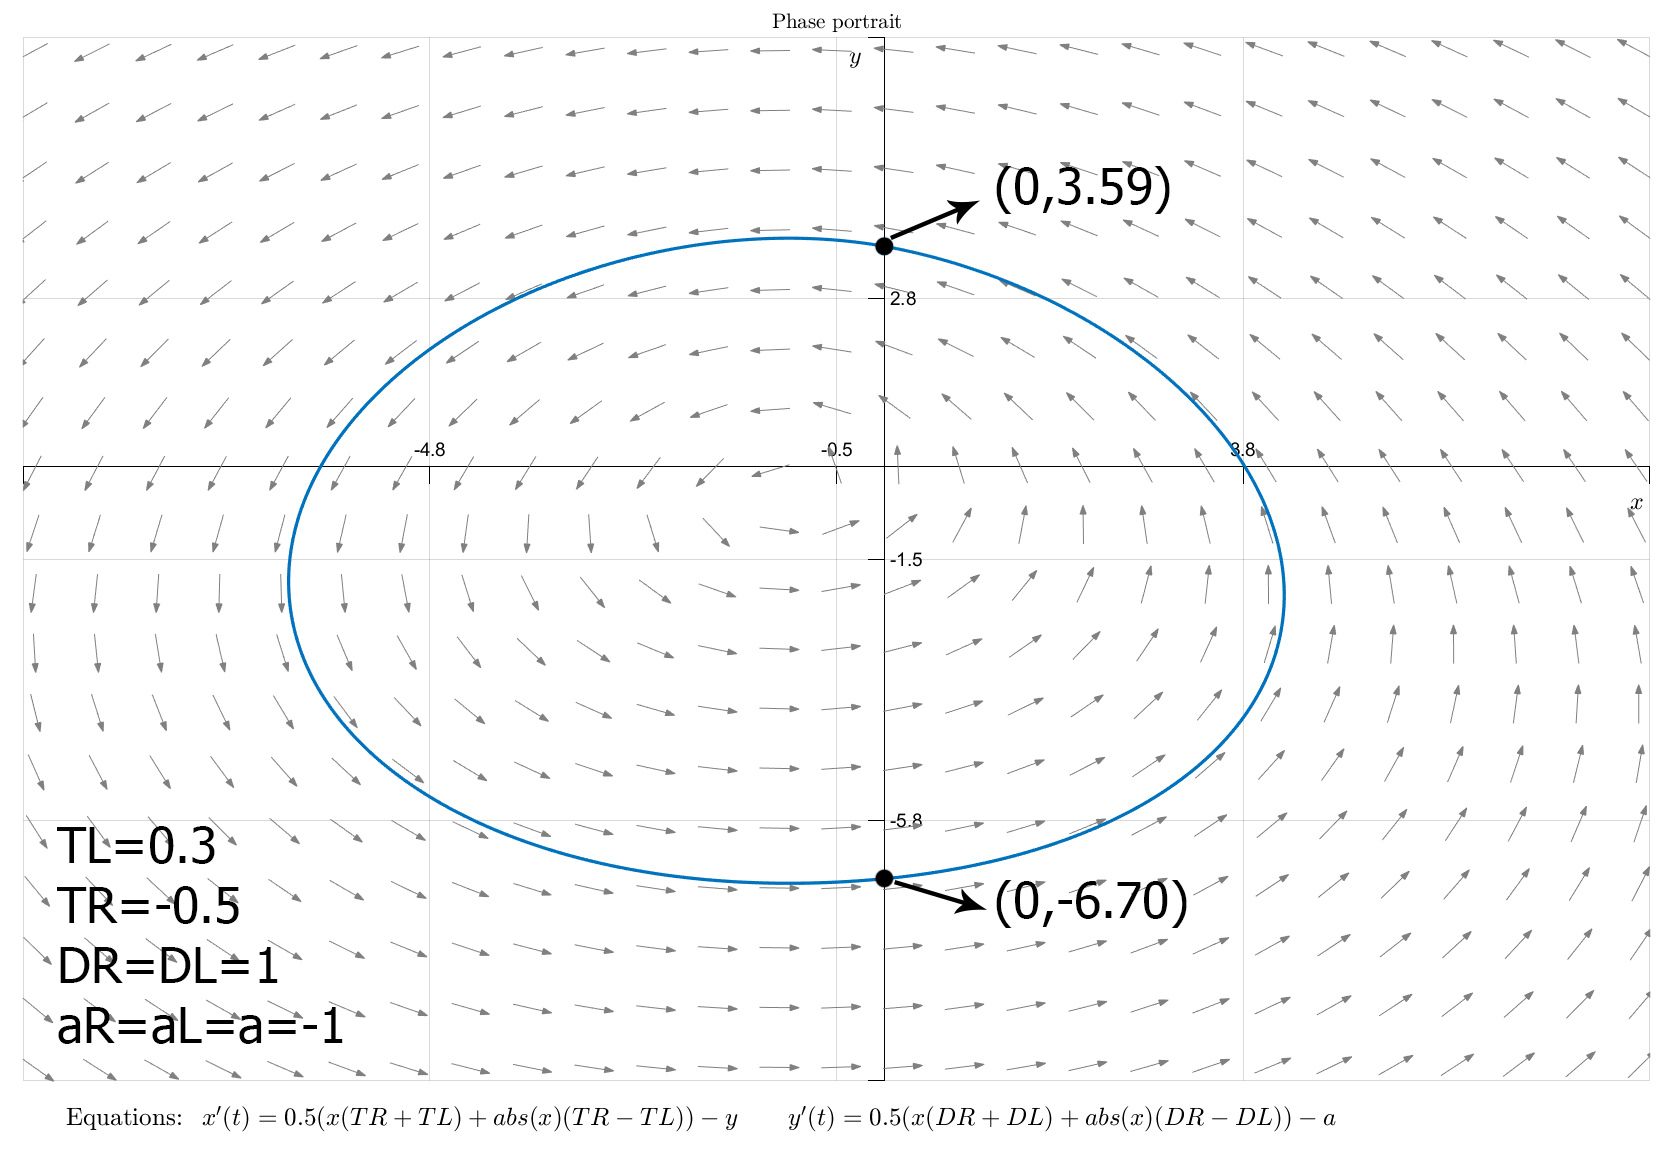
\includegraphics[width=1\textwidth]{clejemplo.jpg}
		\caption{Órbita periódica, cuya existencia hemos establecido previamente con MATLAB}
		\label{fig:clejemplo}
	\end{figure}\smallskip
	
	\vspace{0.5cm} De hecho la solución periódica de la \fref{fig:clejemplo} es un ciclo límite, objeto al que nos dedicaremos en el siguiente capítulo.
	
	\newpage
	
	\chapter{Bifurcación Foco-Centro-Ciclo Límite}
	\label{cap.5}

	La aparición de una oscilación periódica en un sistema dinámico puede darse a través de los fenómenos conocidos como bifurcaciones. Las bifurcaciones son eventos fundamentales que ocurren cuando variamos de manera gradual uno o varios parámetros del sistema, (conocidos como parámetros de control) y esto hace que se produzca un cambio cualitativo en la dinámica del sistema. En esta memoria nos centraremos en una bifurcación específica, de carácter local, donde la modificación de la estabilidad de un punto de equilibrio (mediante la correcta variación de un parámetro de control) origina la aparición de una oscilación periódica aislada, denominada \textit{Ciclo Límite}.

	\vspace{0.5cm}\noindent Esta bifurcación, denominada \textit{Foco-Centro-Ciclo Límite}, es provocada por la variación de la traza de la matriz de uno de los sistemas lineales que definen el sistema lineal a trozos \eref{eq:lienardfinalgr}. Sin embargo, antes de presentar esta bifurcación, es crucial llevar a cabo un análisis detallado del punto de equilibrio y la estabilidad del sistema que estamos investigando. Asimismo, exploraremos el concepto de ciclo límite para luego examinar cómo podemos generar esta bifurcación en nuestro circuito.
	
	\section{Análisis del punto de equilibrio}
	\label{sec:41}
	
		Para llevar a cabo el análisis del punto de equilibrio y de su estabilidad, recordemos primero el sistema que estamos estudiando. Se trata de un sistema dinámico continuo lineal a trozos, específicamente bizonal en su forma canónica de Lienard, tal como se describe en las ecuaciones \eref{eq:lienardfinalgr}.
		
		\vspace{0.5cm}Podemos obtener los puntos de equilibrio de cada una de las zonas igualando a cero el sistema, para la zona izquierda se tendría:

		
		\begin{equation*}
			\begin{pmatrix*}[r]
				0\\ 0
			\end{pmatrix*}= \begin{pmatrix*}[r]
				T_L & -1 \\ D_L & 0
			\end{pmatrix*} \begin{pmatrix*}[r]
				x \\ y
			\end{pmatrix*}-\begin{pmatrix*}[r]
				0 \\ a
			\end{pmatrix*},
		\end{equation*}\smallskip
		
		\begin{equation}
			\label{eq:eqpointL}
			\left\{
			\begin{aligned}
				T_Lx-y=0,\\
				D_Lx-a=0,
			\end{aligned}
			\right. \quad \longrightarrow \left( \overline{x},\overline{y} \right)=\left( \frac{a}{D_L},\frac{aT_L}{D_L} \right). \qquad si \quad D_L\neq0
		\end{equation}\smallskip
		
		\vspace{0.5cm}\noindent Análogamente para la zona derecha se obtendría el punto de equilibrio:
		
		\begin{equation}
			\label{eq:eqpointR}
			\left( \overline{x},\overline{y} \right)=\left( \frac{a}{D_R},\frac{aT_R}{D_R} \right). \qquad si \quad D_R\neq0
		\end{equation}\smallskip
		
		\newpage
		
		En las siguientes figuras veremos la representación gráfica de las posibles posiciones de los puntos de equilibrio \eref{eq:eqpointL} y \eref{eq:eqpointR} en función del signo de $a$
		
		\begin{figure}[h]
			\centering
			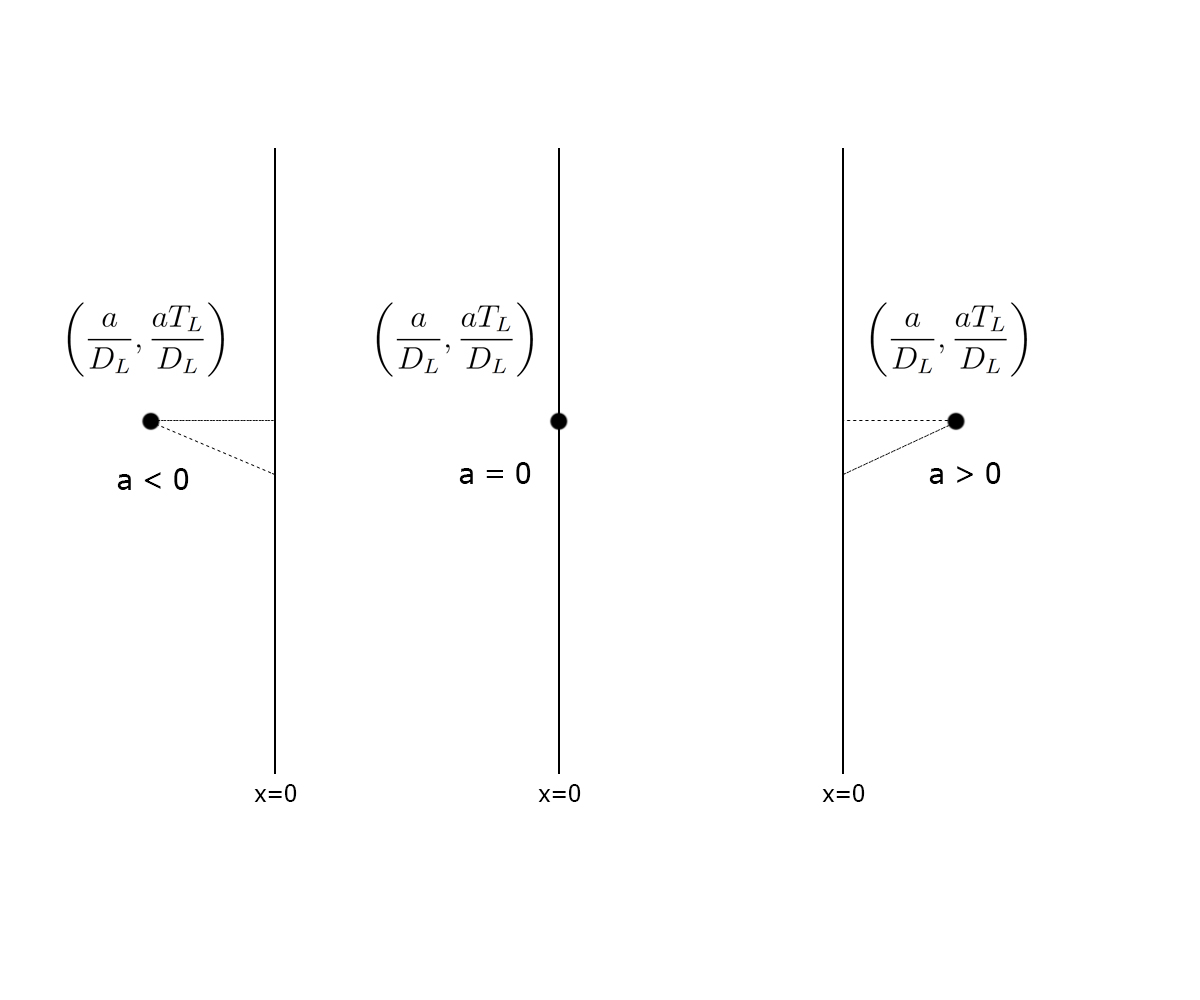
\includegraphics[width=0.7\textwidth,center]{punto.jpg}
			\caption{Posición del punto de equilibrio del sistema lineal de la zona izquierda dependiendo del signo de $a$.}
			\label{fig:punto}
		\end{figure}\smallskip
		

		\begin{figure}[h]
			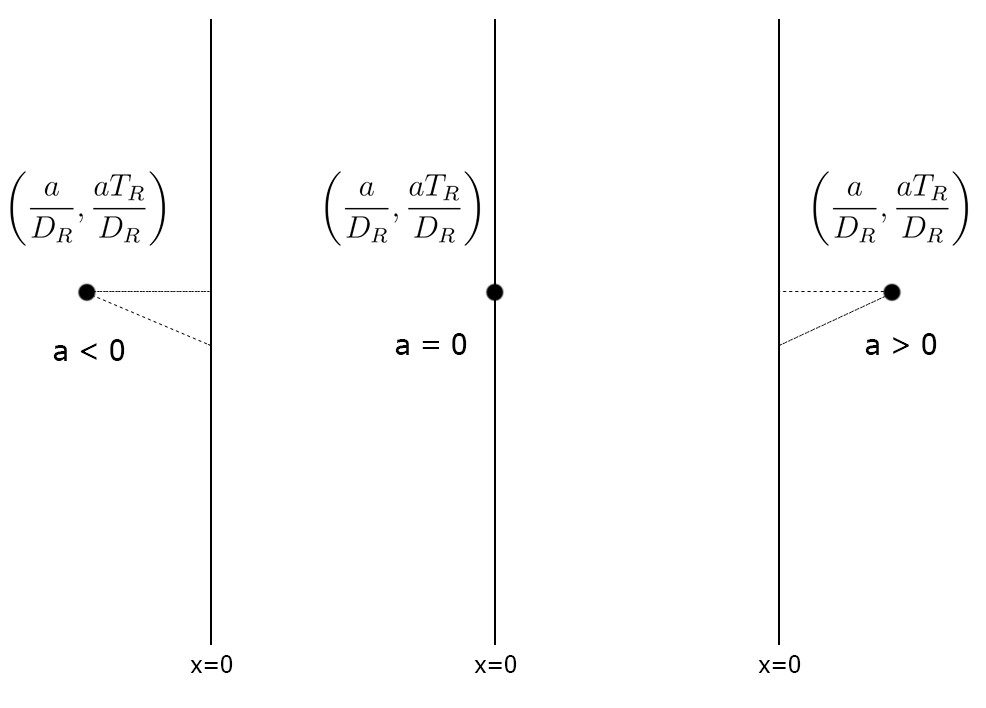
\includegraphics[width=0.7\textwidth,center]{puntoR.jpg}
			\caption{Posición del punto de equilibrio del sistema lineal de la zona derecha dependiendo del signo de $a$.}
			\label{fig:puntoR}
		\end{figure}

\newpage
		
		 Una vez que se ha identificado el punto de equilibrio, se puede proceder a analizar su estabilidad. Este análisis es igual al que ya se realizó en \eref{eq:equilibrio} ya que el polinomio caractrístico es el mismo, por ello veamos directamente las condiciones que se están buscando en este trabajo.
		 
		\vspace{0.2cm}\begin{itemize}
			\item $T_L^2-4\,D_L<0\quad$ por lo que $\quad D_L>0$.
			\item $T_L<0\quad$ para tener un foco asíntoticamente estable.
			\item $T_L=0\quad$ para tener un centro.
			\item $T_L>0\quad$ para tener un foco asíntoticamente inestable.
		\end{itemize}\smallskip
		
		\vspace{0.5cm}Es evidente que un cambio en la estabilidad del punto de equilibrio está directamente relacionado con una modificación en la traza, particularmente en nuestro caso, se refiere a la traza en la zona izquierda. Este ajuste en la traza de nuestro sistema se traducirá en una modificación física del valor de uno o varios componentes del circuito.
		
		\section{Ciclo Límite}
		
		El siguiente concepto crucial que debemos conocer es el de ciclo límite. Un ciclo límite es una solución periódica del sistema que se encuentra aislada del resto de soluciones periódicas, ya sea de manera local o global. A continuación veremos algunas posibles configuraciones de estabilidad que se pueden dar en un ciclo límite.
		
		\newpage
		
		\noindent{\Large\textbullet\quad Ciclo Límite Asintóticamente Estable}
		
		\vspace{0.5cm}Independientemente de si seleccionamos las condiciones iniciales dentro o fuera del ciclo límite, las trayectorias de las soluciones cercanas a dicho ciclo límite convergen a él.
		
		\begin{figure}[h]
			\centering
			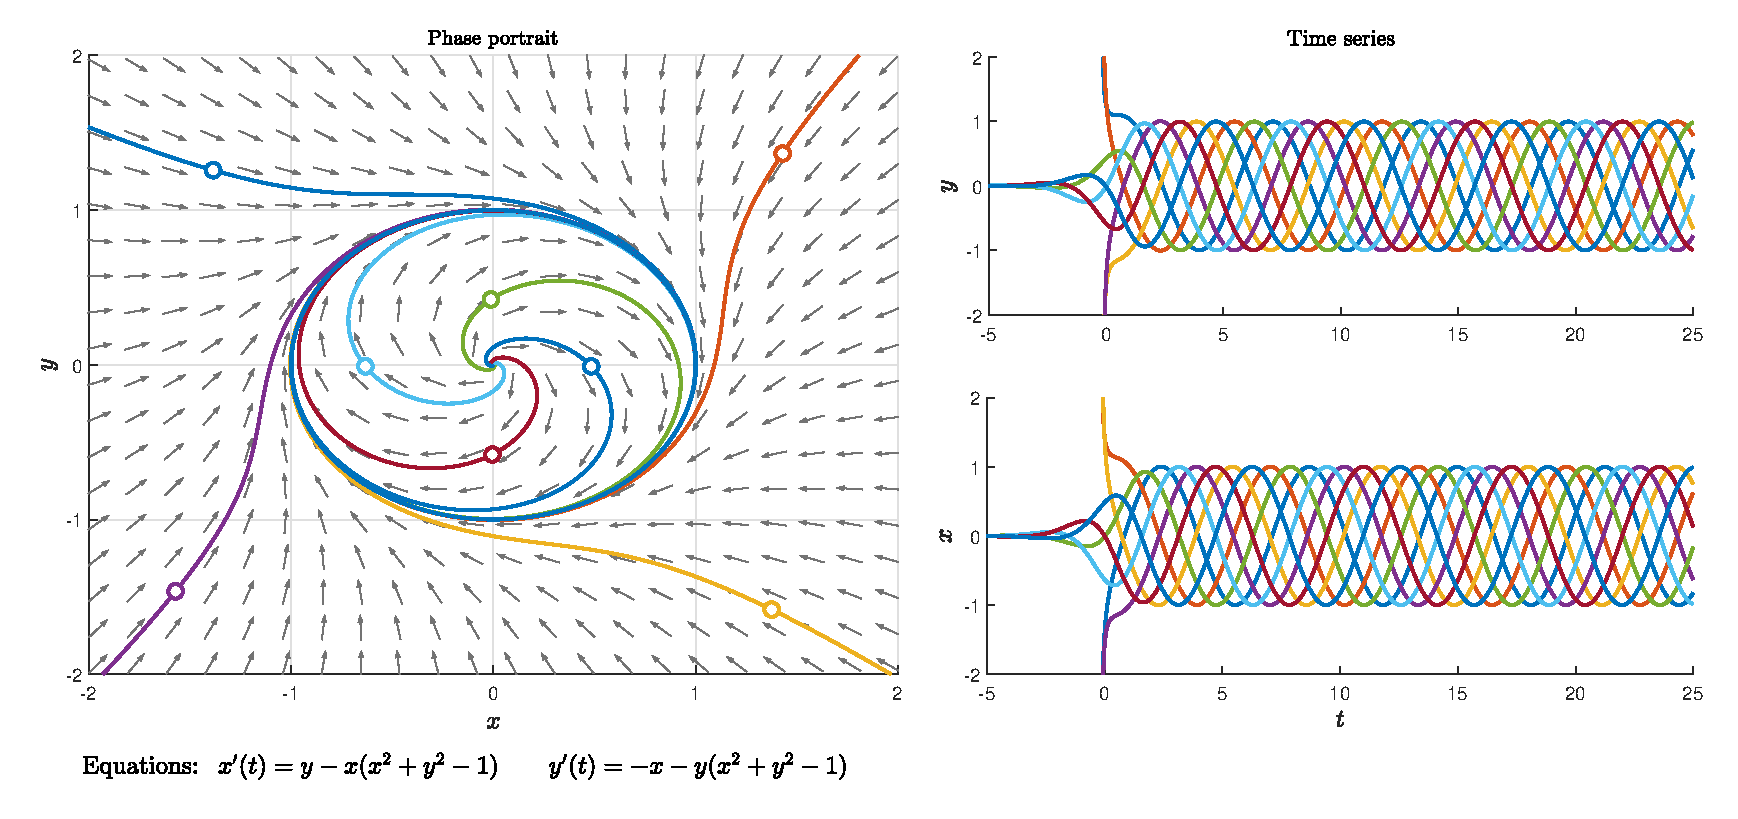
\includegraphics[width=1\textwidth]{cle.eps}
			\caption{Ciclo límite asintóticamente estable.}
			\label{fig:cle}
		\end{figure}\smallskip
		
	\vspace{1cm}\noindent{\Large\textbullet\quad Ciclo Límite Inestable}
	
	\vspace{0.5cm}Si optamos por condiciones iniciales cercanas al Ciclo Límite (dentro o fuera), las trayectorias de las soluciones no convergen a él.
	
	\begin{figure}[h]
		\centering
		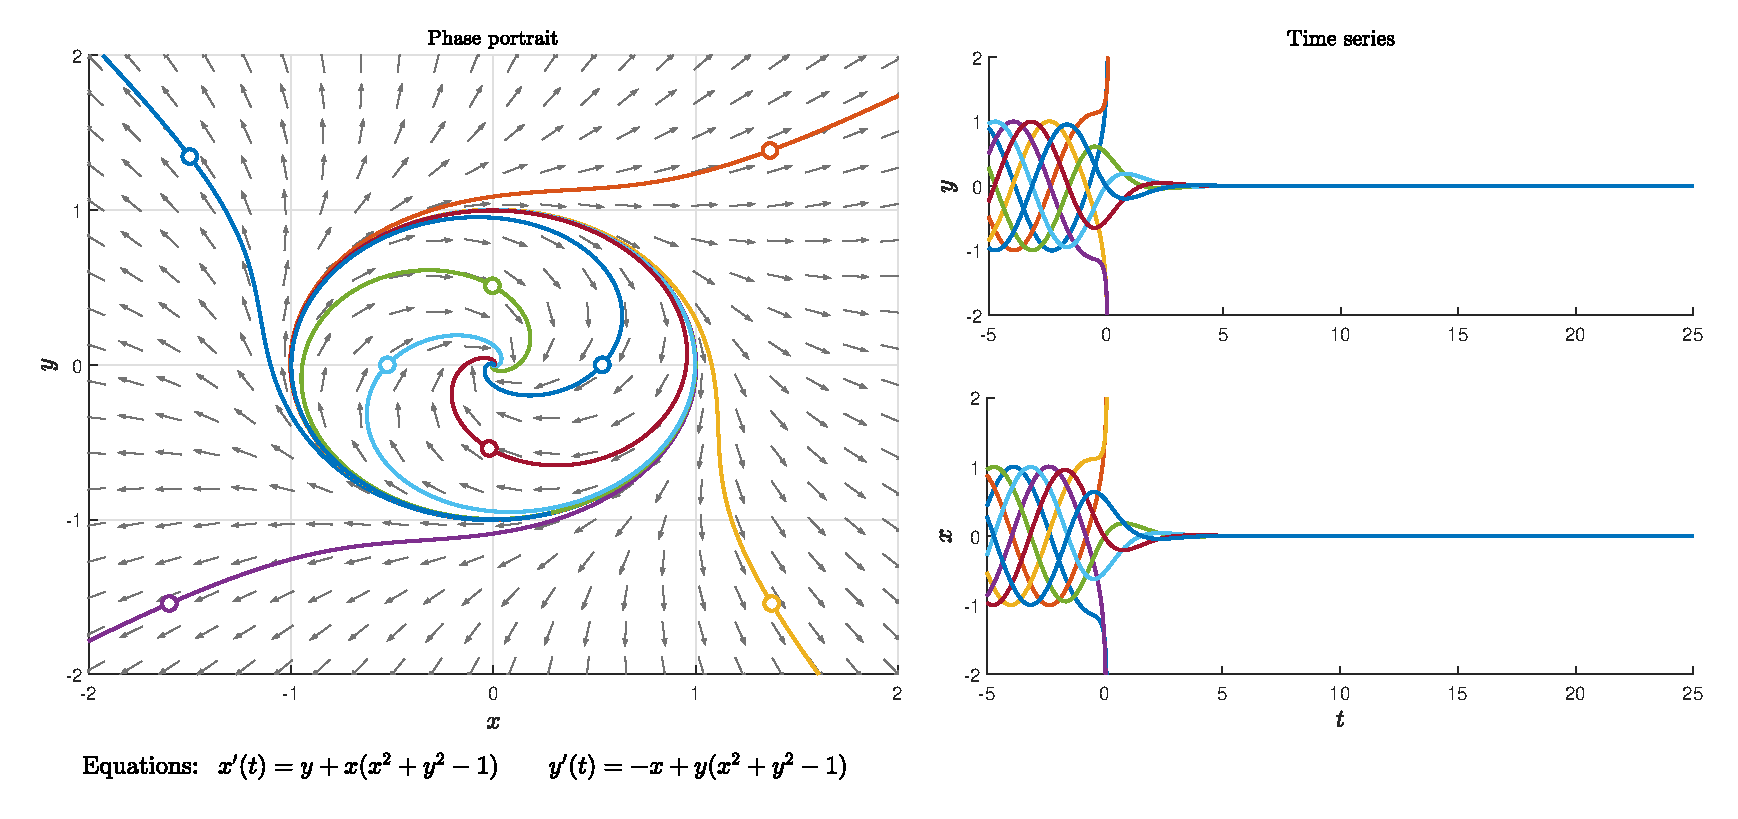
\includegraphics[width=1\textwidth]{cli.eps}
		\caption{Ciclo límite inestable.}
		\label{fig:cli}
	\end{figure}\smallskip
	
	\newpage
	
	\vspace{0.5cm}\noindent{\Large\textbullet\quad Ciclo Límite Semiestable}
	
	\vspace{0.5cm}Esta configuración se da cuando solo las soluciones con condiciones iniciales dentro o fuera, y cercanas, al ciclo límite convergen hacia el mismo.
	
	\begin{figure}[h]
		\centering
		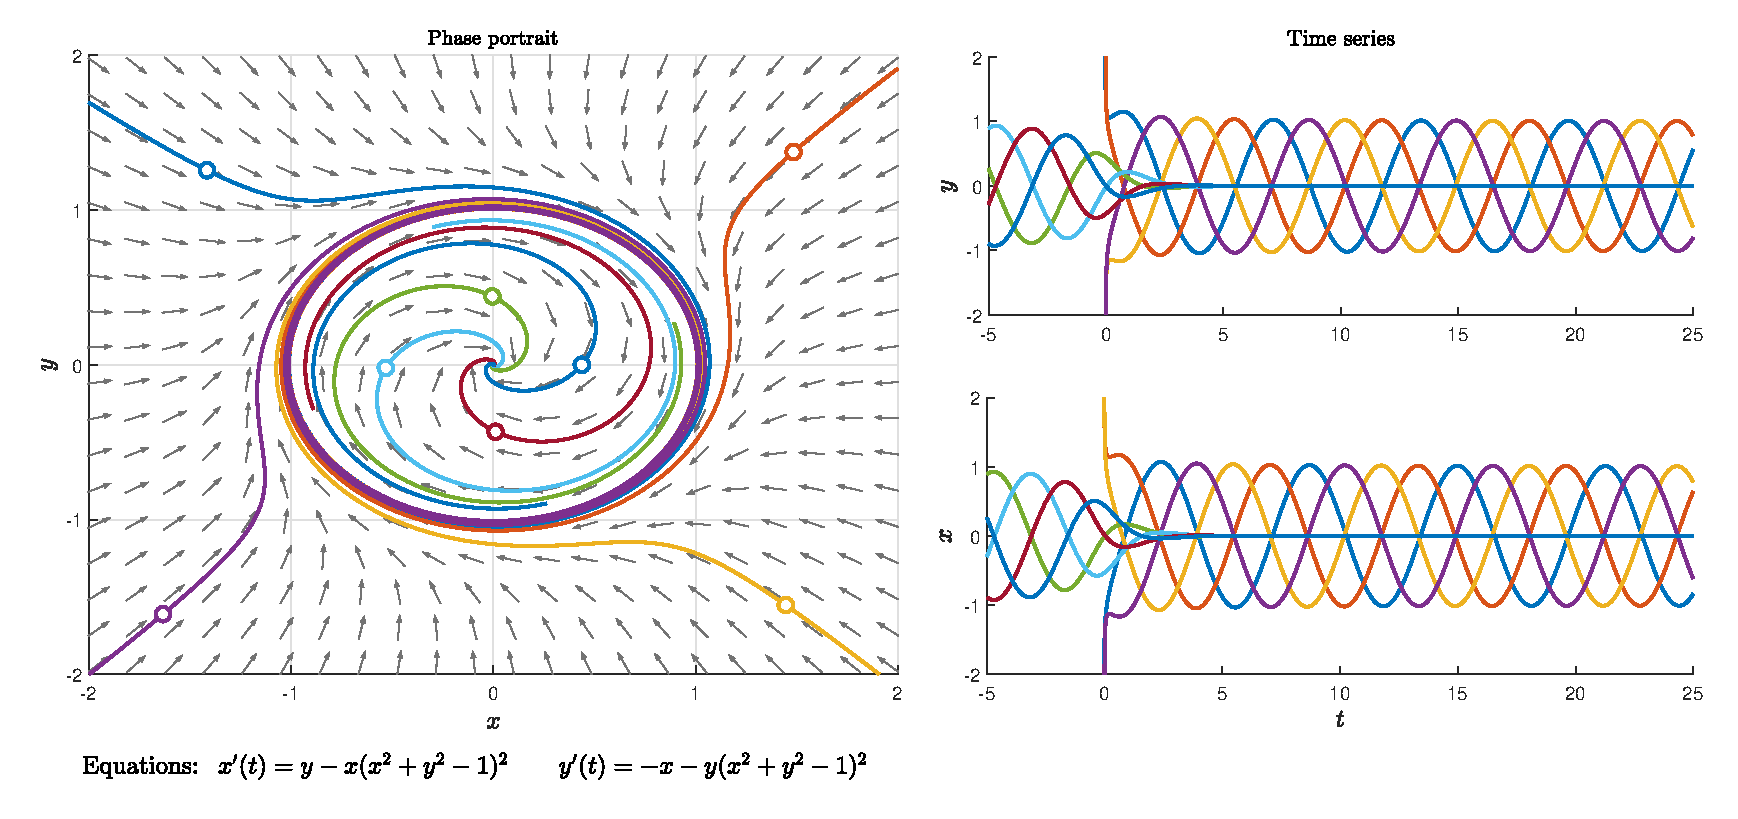
\includegraphics[width=1\textwidth]{clpe.eps}
		\caption{Ciclo límite semiestable donde solo las soluciones con condiciones iniciales cercanas y fuera del ciclo límite convergen hacia él.}
		\label{fig:clpe}
	\end{figure}\smallskip
	
	\vspace{0.5cm} El ciclo límite de mayor interés para nuestro trabajo es el asintóticamente estable (ver \fref{fig:cle}), dado que, sin importar dónde seleccionemos las condiciones iniciales, siempre y cuando sean cercanas al ciclo límite, la solución convergerá hacia la oscilación periódica. Además, en caso de que nuestro sistema sufra alguna perturbación que lo aleje de la oscilación periódica, este tiende a regresar y restablecer dicha oscilación.
	
	\vspace{0.5cm}Por otro lado el ciclo límite inestable (ver \fref{fig:cli}) es altamente desfavorable ya que la única opción de que la solución de nuestro sistema alcance al ciclo límite es estableciendo las condiciones iniciales exactas para ello, lo cual es altamente complicado.
	
	\vspace{0.5cm} Por último, el ciclo limite semiestable (ver \fref{fig:clpe}) tampoco nos es de interés ya que aunque consigamos establecer las condiciones iniciales adecuadas para que la solución de nuestro sistema converga al ciclo límite, dicha solución puede perder la estabilidad con cierta facilidad
	
	\newpage
	
	\section{Bifurcación foco-centro-ciclo límite y su determinación a partir de la carterización integral de la semiaplicación de Poincaré}
	
	\begin{comment}
	o de los Ciclos Límites ha sido históricamente realizado de manera específica para cada sistema. Por lo general, este proceso implica investigar el punto de equilibrio y su estabilidad, analizar si existe una oscilación periódica y finalmente verificar que esta oscilación periódica esté aislada, lo cual puede ser un desafío. En nuestro caso, no es necesario realizar este tipo de análisis exhaustivo debido a que hemos sido capaces de reformular nuestro sistema \eref{eq:sistema1} en la forma \eref{eq:sis2ec} y, posteriormente, en la forma \eref{eq:lienardrl}.
	\end{comment}
	
	Existen trabajos previos que han abordado la existencia de la bifurcación foco-centro-ciclo límite en sistemas lineales a trozos. Estos trabajos se pueden consultar en: el Capítulo \textit{``The Focus-Center-Limit Cycle Bifurcation in Discontinuous Planar Piecewise Linear
	Systems Without Sliding''} de \cite{ciclolimite} y las Secciones 8.1 y 3.6 de \cite{amarillo}, específicamente el Teorema 3.27 de este último. En esos trabajos se ha realizado un análisis del problema diferente al nuestro, nosotros aplicaremos la caracterización integral que hemos explorado previamente. Mediante el cumplimiento de una serie de requisitos en los parámetros del sistema, los cuales se explicitarán más adelante, podremos lograr un cambio en la estabilidad del punto de equilibrio, pasando de foco asintóticamente estable a centro y, finalmente, a foco inestable. Este proceso nos llevará a obtener el ciclo límite asintóticamente estable, lo que representa nuestra oscilación periódica.
	
	\vspace{0.5cm} Enunciaremos a continuación el resultado principal que garantiza la existencia de la bifurcación y la aparición del ciclo límite bizonal.
	
	\begin{theorem}
		\label{teo:5.1}
		Considerando el sistema \eref{eq:lienardfinalgr}, donde tomamos $T_L$ como parámetro de bifurcación (esto es, suponemos que el resto de parámetros permanecen fijos), elegimos $a<0$ y $D_L>0$. El sistema experimenta una bifurcación foco-centro-ciclo límite al pasar $T_L$ por el valor cero. Es decir, de la configuración de centro para $T_L=0$,ver \fref{fig:centro2}, se produce un ciclo límite (que nace de la órbita periódica del centro que es tangente a la sección de Poincarè) cuando $T_L T_R<0$ y $\mid T_L \mid$ es lo suficientemente pequeño. El ciclo límite que nace es asintóticamente estable si $T_L>0$, ver \fref{fig:cle}, e inestable cuando $T_L<0$, ver \fref{fig:cli}. Además, se puede calcular el periodo $T_P$ de la oscilación como:
		
		\begin{equation}
			\label{eq:tperiodo}
			T_P= \frac{4\pi}{D_L\sqrt{4D_L^2-T_L^2}}+\frac{2(D_R-D_L-2T_R^2+T_RT_L+T_L^2)}{a^3}\left[\left( \frac{3\, a^3 \, \pi}{2\, D_L^{3/2}\, T_R} \right)\cdot \left(T_L\right)+\cdots\right].
		\end{equation}\smallskip
		
		\noindent Y la amplitud $\varDelta$ (medida como la distancia entre los puntos de corte de la órbita periódica con la recta de separación) viene dada por:
		
		\begin{equation}
			\label{eq:amplitu}
			\scalebox{0.95}{$\displaystyle
				\begin{split}
					\varDelta = &\left( \left( \frac{3a^3 \pi}{2D_L^{3/2}T_R} \right)^{1/3} \cdot (T_L)^{1/3} + \cdots \right) - \left[ -\left( \left( \frac{3a^3 \pi}{2D_L^{3/2}T_R} \right)^{1/3} \cdot (T_L)^{1/3} + \cdots \right) \right.-\\
					&\frac{2T_R}{3a} \left( \left( \frac{3a^3 \pi}{2D_L^{3/2}T_R} \right)^{1/3} \cdot (T_L)^{1/3} + \cdots \right)^2 - \left. \frac{4T_R^2}{9a^2} \left( \left( \frac{3\, a^3 \, \pi}{2\, D_L^{3/2}\, T_R} \right)\cdot \left(T_L\right)+\cdots \right) + \cdots \right]
				\end{split}
				$}
		\end{equation}
	\end{theorem}
	
	\newpage
	
	Veamos las condiciones para que se deben cumplir en nuestras ecuaciones y sus consecuencias para que se cumpla el Teorema \ref{teo:5.1} en nuestro sistema \eref{eq:lienardfinalgr}:
		\begin{itemize}
			\item $a<0$ para que el punto de equilibrio de la zona izquierda esté contenido en la zona $x<0$, ver \fref{fig:punto}.
			\item Ya que $a<0$ y queremos que el polinomio característico  tenga raices imaginarias para tener una configuración de foco en nuestro punto de equilibrio, debemos tener $T_L^2-4\,D_L<0$ y $D_L>0$, ver Sección \ref{sec:41}.
			\begin{comment}
			\item Como hemos establecido $a_R<0$, el posible punto de equilibrio de la zona Derecha estaría ubicado en la zona $x<0$, ver \eref{eq:eqpointR}, por ello podemos elegir:\begin{itemize}
				\item No hay punto de equilibrio $\rightarrow D_R=0$ 
				\item Si hay punto de equilibrio y es virtual $\rightarrow D_R\neq0$ 
			\end{itemize}
			\end{comment}

			\item Nuestro parámetro de bifurcación será $T_L$, por ello lo haremos variar de negativo a positivo haciendolo pasar por cero, $T_L<0 \rightarrow T_L=0 \rightarrow T_L>0$ y siempre para un valor pequeño de $\mid T_L \mid$. Lo hacemos de esta manera para que el ciclo límite que obtengamos sea asintóticamente estable.
			\item Del Teorema \ref{teo:5.1} tenemos que $T_LT_R<0$ con $T_L>0$, por ello  $T_R<0$.
		\end{itemize}
		
		
	\vspace{0.5cm} En las siguientes figuras vemos gráficamente como se produce la bifurcacion tomando como parámetro de control $T_L$.
		
	\newpage
	
	\begin{figure}[h]
		\centering
		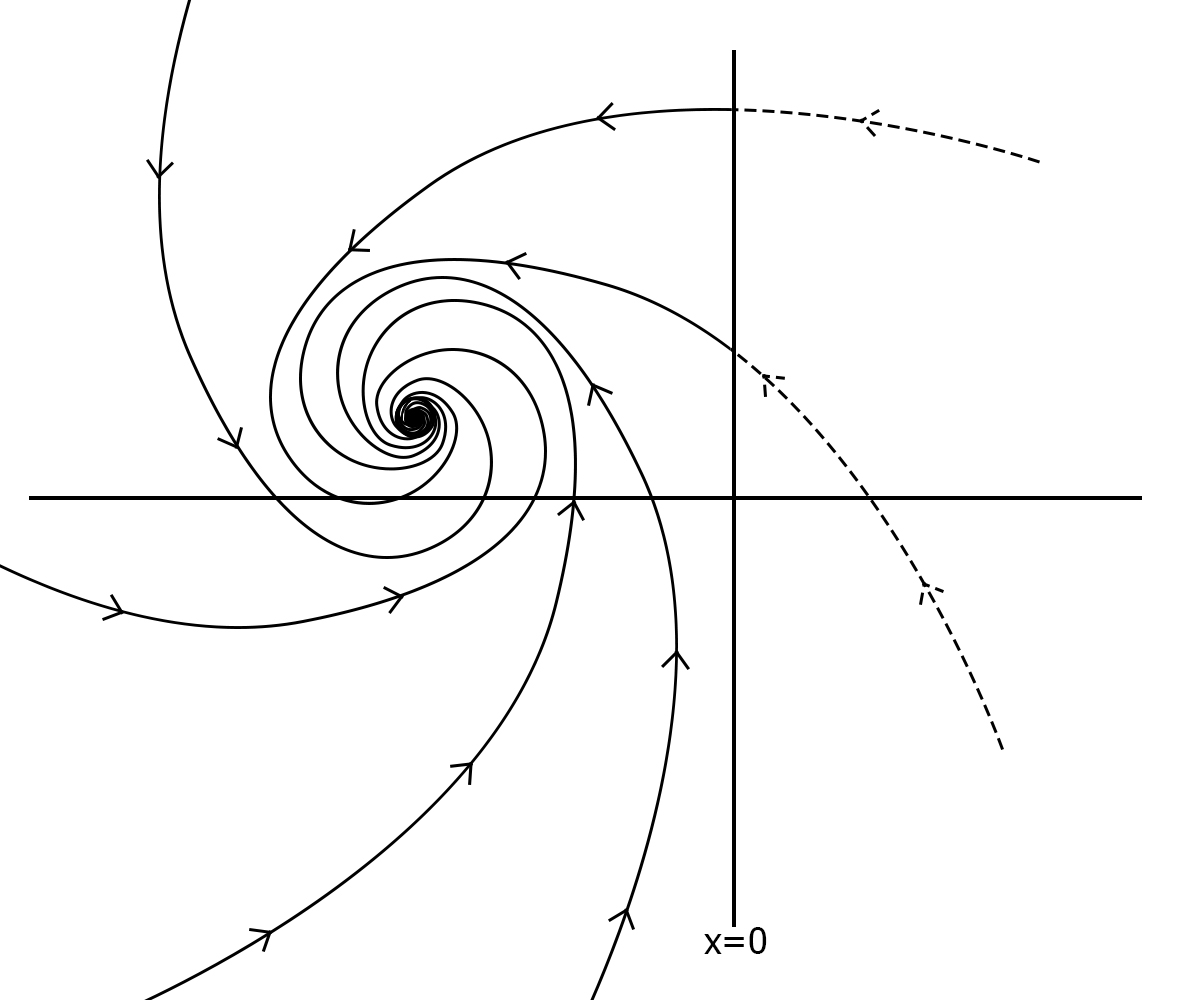
\includegraphics[width=1.1\textwidth,center]{foco3x=0.jpg}
		\caption{Foco asintóticamente estable con sección de Poincaré en $x=0$.}
		\label{fig:foco3}
	\end{figure}\smallskip
	
	\newpage
	
	\begin{figure}[h]
		\centering
		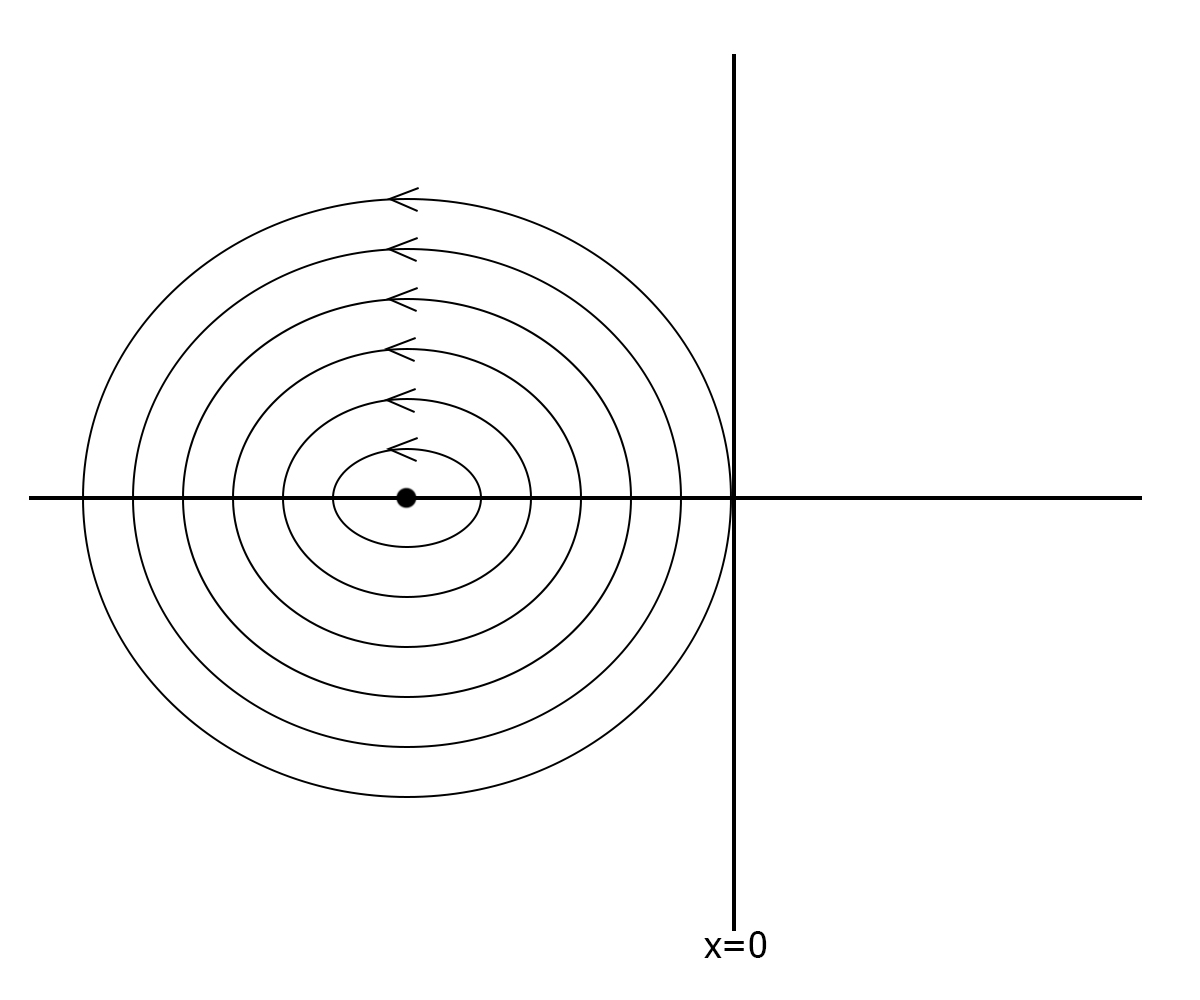
\includegraphics[width=1.1\textwidth,center]{centro2x=0.jpg}
		\caption{Centro con Sección de Poincaré en $x=0$.}
		\label{fig:centro2}
	\end{figure}\smallskip
	
	\newpage
	
	\begin{figure}[h]
		\centering
		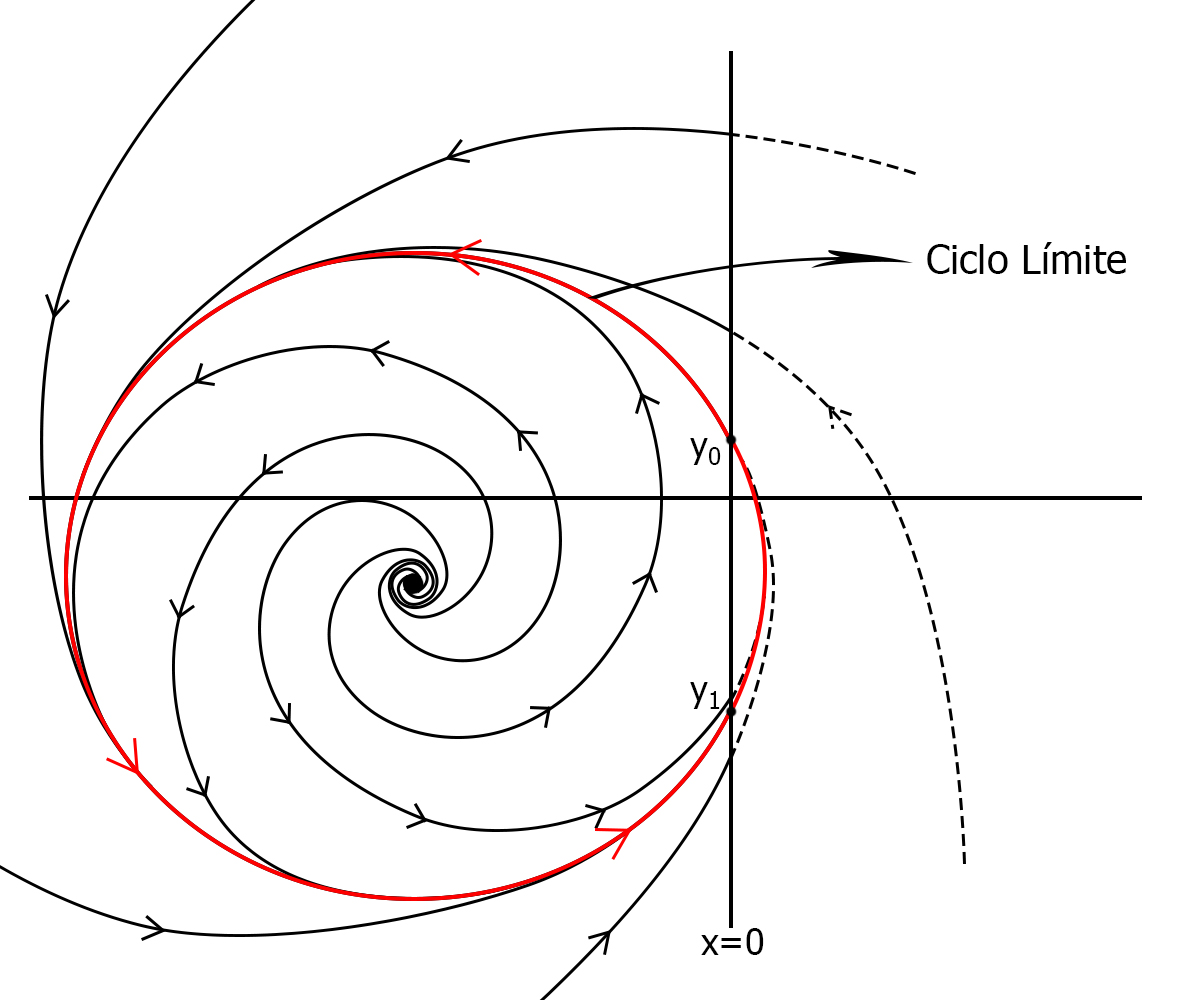
\includegraphics[width=1.1\textwidth,center]{ciclolimite3x=0_v2.jpg}
		\caption{Ciclo límite asintóticamente estable con Sección de Poincaré en $x=0$.}
		\label{fig:ciclolimite3}
	\end{figure}\smallskip
	
	\newpage
	
	Para la demostración del Teorema \ref{teo:5.1} haremos uso de la Caracterización Integral de la semiaplicación de Poincaré, desarrollos en series de MacLaurin y el \textit{Teorema de la Función Implícita}, este último se puede consultar más en profundidad en \cite{tf1}. Presentaremos a continuación este último conocido teorema.
	
	\begin{theorem}[Función Implícita]
		\label{teo.fi}
		Sean $f:\mathbb{R}^2 \longrightarrow\mathbb{R}$ con derivadas parciales de primer orden continuas, y $(x_0,y_0) \in \mathbb{R}^2$ tales que
		
		\begin{equation*}
			f(x_0,y_0)=0, \qquad\frac{\partial f}{\partial y}(x_0,y_0)\neq 0
		\end{equation*}\smallskip
		
		\noindent entonces existe una función $g$ definida en un intervalo abierto $I$ que contiene a $x_0$, de forma que $y_0=g(x_0)$ y
		
		\begin{equation*}
			\scalebox{1}{$\displaystyle
			f(x,g(x))=0. \qquad \forall \: x\in I
			$}
		\end{equation*}\smallskip
		
		\noindent es más, $g$ es derivable y tiene derivada continua en $I$.
		
	\end{theorem}
	
	\vspace{0.5cm}\noindent Ahora veremos la demostración del Teorema \ref{teo:5.1}.
	\begin{proof}[\textbf{Demostración}](del Teorema \ref{teo:5.1})
		\label{dem5.1}
	Es obvio que el sistema \eref{eq:lienardfinalgr} posee una órbita periódica transversal a la linea de separación $x=0$, como la de la \fref{fig:aplipoincareL-Rcerrado}, si y solo si el sistema de ecuaciones
	
	\begin{equation}
		\label{eq:cierre}
		\scalebox{1}{$\displaystyle
			\left\{
			\begin{aligned}
				PV\left\{\int_{y_1}^{y_0}\frac{-y}{D_Ly^2-aT_Ly+a^2}dy\right\}&=\frac{k_L\pi T_L}{D_L\sqrt{4D_L-T_L^2}},
				\\[2mm]
				PV\left\{\int_{y_1}^{y_0}\frac{-y}{D_Ry^2-aT_Ry+a^2}dy\right\}&=\frac{-k_R\pi T_R}{D_L\sqrt{4D_L-T_L^2}}.
			\end{aligned}
			\right. 
			$}
	\end{equation}\smallskip
	
	\vspace{0.5cm}\noindent posee una solución $y_0=y_0^*>0$ e $y_1=y_1^*<0$.
	
	\vspace{0.5cm}\noindent Demostraremos, aplicando el teorema de la función implícita (Teorema \ref{teo.fi}), que el sistema \eref{eq:cierre} posee solución bajo la hipótesis del teorema. Fijaremos los siguientes parámetros constantes en nuestro sistema: $D_L$, $D_R$, $a$, $k_L$, $k_R$, $T_R$, con $a<0$ por lo que $k_L$ y $k_R$ serían $k_L=2$ y $k_R=0$. Luego, \eref{eq:cierre} se escribe como:
	
	\begin{comment}
	
	\begin{equation}
		\label{eq:cierre2}
		\scalebox{1}{$\displaystyle
			\left\{
			\begin{aligned}
				&\int_{y_1}^{y_0}\frac{-y}{D_Ly^2-aT_Ly+a^2}dy-\frac{2\pi T_L}{D_L\sqrt{4D_L-T_L^2}}=0,
				\\[2mm]
				&\int_{y_1}^{y_0}\frac{-y}{D_Ry^2-aT_Ry+a^2}dy=0,
			\end{aligned}
			\right. 
			$}
	\end{equation}\smallskip
\end{comment}
	
	\begin{equation}
		\label{eq:cierre3}
		\scalebox{1}{$\displaystyle
			\left\{
			\begin{aligned}
				&F_1(y_0,y_1,T_L)&=0,
				\\[2mm]
				&F_2(y_0,y_1)&=0,
			\end{aligned}
			\right. 
			$}
	\end{equation}\smallskip
	
	\noindent donde
	
	\begin{equation}
		\label{eq:aux1}
		F_1(y_0,y_1,T_L)=\int_{y_1}^{y_0}\frac{-y}{D_Ly^2-aT_Ly+a^2}dy-\frac{2\pi T_L}{D_L\sqrt{4D_L-T_L^2}},
	\end{equation}\smallskip
	
	\noindent y
	
	\begin{equation}
		\label{eq:aux2}
		F_2(y_0,y_1)=\int_{y_1}^{y_0}\frac{-y}{D_Ry^2-aT_Ry+a^2}dy.
	\end{equation}\smallskip
	
	\noindent Desde la ecuación \eref{eq:aux2}, aplicando la Proposición 3.1 de \cite{properties}, obtenemos que:
	
		\begin{equation}
		\label{eq:macla}
		\scalebox{1}{$\displaystyle
			y_1=-y_0-\frac{2T_R}{3a}y_0^2-\frac{4T_R^2}{9a^2}y_0^3+\cdots
			$}
	\end{equation}\smallskip
	
	\noindent Haciendo uso de \eref{eq:macla}, se puede escribir la primera expresion de \eref{eq:cierre3} de la siguente manera
	
	\begin{equation}
		\label{eq:f1nuevo}
		\tilde{F}_1(y_0,T_L)=0.
	\end{equation}\smallskip
	
	\noindent donde
	
	\begin{equation}
		\label{eq:macla2}
				\tilde{F_1}(y_0,T_L)=\int_{-y_0-\frac{2T_R}{3a}y_0^2+...}^{y_0}\frac{-y}{D_Ly^2-aT_Ly+a^2}dy-\frac{2\pi T_L}{D_L\sqrt{4D_L-T_L^2}},
	\end{equation}\smallskip

	\noindent como se cumple
	
	\begin{equation}
		\label{dpar}
		\tilde{F_1}(0,0)=0, \quad \text{y}\quad\frac{\partial \tilde{F_1}}{\partial T_L}(0,0)=\frac{\pi}{D_L^{3/2}}\neq0.
	\end{equation}\smallskip
	
	\noindent aplicando el teorema de la función implícita (Teorema \ref{teo.fi}), existe una única función que nos permite definir $T_L=f_1(y_0)$ de manera local. El desarrollo en series de MacLaurin de esta función es:
	
	\begin{equation}
		\label{macla3}
		T_L=\frac{2\, D_L^{3/2}\, T_R}{3\, a^3 \, \pi}\: y_0^3+\frac{2\, D_L^{3/2}\, T_R^2}{9\, a^4 \, \pi}\: y_0^4-\cdots
	\end{equation}\smallskip
	
	\noindent Realizando una inversión de la serie  anterior podemos finalmente definir $y_0=f_1(T_L)$:
	
	\begin{equation}
		\label{eq:macla4}
		\begin{aligned}
		&y_0^3= \left( \frac{3\, a^3 \, \pi}{2\, D_L^{3/2}\, T_R} \right)\cdot \left(T_L\right)+\cdots,\\[3mm]
		&y_0= \left( \frac{3\, a^3 \, \pi}{2\, D_L^{3/2}\, T_R} \right)^{1/3}\cdot \left(T_L\right)^{1/3}+\cdots \qquad \text{para} \quad T_R \neq 0
	\end{aligned}
	\end{equation}
	
	\vspace{0.5cm}\noindent siempre y cuando $T_R\neq0$.
	
		\begin{comment}
	\vspace{0.5cm}Se puede calcular el periodo de la oscilación mediante la obtención de los semitiempos de vuelo izquierdo y derecho, nuevamente la obtención de estas expresiones se escapa de los objetivos de este trabajo por lo que  únicamente las presentaremos. Se puede consultar el Teorema 19 de \cite{caracterizacion} para profundizar más en este apartado.
	
	\vspace{0.5cm} Definiremos el periodo de la oscilación $T_P$ como la suma del semitiempo de vuelo izquierdo $\tau_L$ y el semitiempo de vuelo derecho $\tau_R$. A continuación veremos las expresiones de los semitiempos de vuelo prsentadas en \cite{caracterizacion}.
	


	\vspace{0.5cm}\noindent Semitiempo de vuelo izquierdo
	
	\begin{equation}
		\label{eq:semitiempoL}
		\scalebox{1.2}{$\displaystyle
		\tau_L=\frac{4\pi}{D_L\sqrt{4D_L^2-T_L^2}}+\int_{y_1}^{y_0}\frac{a_L}{D_Ly^2-aT_Ly+a^2}dy.
		$}
	\end{equation}\smallskip
	
	\vspace{0.5cm}\noindent Semitiempo de vuelo derecho
	
	\begin{equation}
		\label{eq:semitiempoR}
		\scalebox{1.2}{$\displaystyle
		\tau_R=\int_{y_1}^{y_0}\frac{-a_R}{D_Ry^2-aT_Ry+a^2}dy.
		$}
	\end{equation}\smallskip
		\end{comment}
	\vspace{0.5cm} El periodo $T_P$ se calculará como la suma del semitiempo de vuelo izquierdo $\tau_L$ y el semitiempo de vuelo derecho $\tau_R$, los cuales tienen las siguientes expresiones:
		
		\begin{equation}
			\label{eq:semitiempoL}
			\scalebox{1}{$\displaystyle
				\tau_L=\frac{4\pi}{D_L\sqrt{4D_L^2-T_L^2}}+\int_{y_1}^{y_0}\frac{a}{D_Ly^2-aT_Ly+a^2}dy,
				$}
		\end{equation}\smallskip
		
		\begin{equation}
			\label{eq:semitiempoR}
			\scalebox{1}{$\displaystyle
				\tau_R=\int_{y_1}^{y_0}\frac{-a}{D_Ry^2-aT_Ry+a^2}dy.
				$}
		\end{equation}\smallskip
	
	\noindent Recordemos que los parámetros $D_L$, $D_R$, $a$ y $T_R$ están fijos, por lo que las expresiones \eref{eq:semitiempoL} y \eref{eq:semitiempoR} dependen únicamente de $y_0$ e $y_1$. Como ya se ha visto  anteriormente se puede escribir $y_1=f(y_0)$ e $y_0=f(T_L)$, por lo que las expresiones \eref{eq:semitiempoL} y \eref{eq:semitiempoR} tan solo dependerán de $T_L$. A continuación presentaremos el desarrollo en series que hemos calculado para cada semitiempo de vuelo, donde hemos sustitudo $y_1$ por la expresión en función de $y_0$ que vimos en \eref{eq:macla}:
	
	\begin{equation}
		\label{eq:seriestL}
		\tau_L=\frac{4\pi}{D_L\sqrt{4D_L^2-T_L^2}}+\frac{2y_0}{a}-\frac{2T_Ry_0^2}{3a^2}+\frac{(4a^2T_R^2+6a(aT_RT_L+a(-D_L+T_L^2)))y_0^3}{9a^5}+\cdots
	\end{equation}\smallskip
	
	\begin{equation}
		\label{eq:seriestR}
		\tau_R=-\frac{2y_0}{a}+\frac{2T_Ry_0^2}{3a^2}+\frac{2(3D_R-8T_R^2)y_0^3}{9a^3}+\cdots
	\end{equation}\smallskip
	
\noindent Sumando los semitiempos anteriores obtenemos el periodo:
	
	\begin{equation}
		T_P=\tau_L + \tau_R = \frac{4\pi}{D_L\sqrt{4D_L^2-T_L^2}}+\frac{2(D_R-D_L-2T_R^2+T_RT_L+T_L^2)y_0^3}{a^3}.
	\end{equation}\smallskip
	
	\noindent Y sustituyendo en la anterior ecuación $y_0$ por la expresión en función de $T_L$ que se presentó en \eref{eq:macla4}, obtenemos la expresión del periodo \eref{eq:tperiodo}, donde $T_P$ únicamente depende de $T_L$.
	
 	\vspace{0.5cm}El cálculo de la amplitud $\varDelta$ se puede hacer con las expresiones \eref{eq:macla} y \eref{eq:macla4} de la siguiente manera:
	
	\begin{equation}
		\varDelta=y_0-y_1=\left( \left( \frac{3\, a^3 \, \pi}{2\, D_L^{3/2}\, T_R} \right)^{1/3}\cdot \left(T_L\right)^{1/3}+\cdots \right) - \left[ -y_0-\frac{2T_R}{3a}y_0^2-\frac{4T_R^2}{9a^2}y_0^3+\cdots \right]
	\end{equation}\smallskip
	
	\noindent Sustituyendo en la anterior ecuación $y_0$ por la expresión \eref{eq:macla4}, como ya se hizo anteriormente, se obtiene la expresión de la amplitud \eref{eq:amplitu}, la cual depende únicamente de $T_L$.
	
	\begin{comment}
	
\begin{equation}
	\scalebox{0.95}{$\displaystyle
   		\begin{split}
		&\varDelta = \left( \left( \frac{3a^3 \pi}{2D_L^{3/2}T_R} \right)^{1/3} \cdot (T_L)^{1/3} + \cdots \right) - \left[ -\left( \left( \frac{3a^3 \pi}{2D_L^{3/2}T_R} \right)^{1/3} \cdot (T_L)^{1/3} + \cdots \right) \right. \ddots\\
		&\ddots - \frac{2T_R}{3a} \left( \left( \frac{3a^3 \pi}{2D_L^{3/2}T_R} \right)^{1/3} \cdot (T_L)^{1/3} + \cdots \right)^2 - \left. \frac{4T_R^2}{9a^2} \left( \left( \frac{3\, a^3 \, \pi}{2\, D_L^{3/2}\, T_R} \right)\cdot \left(T_L\right)+\cdots \right) + \cdots \right]
  	 	\end{split}
 	$}
\end{equation}
\end{comment}

\vspace{0.5cm} Con esto queda finalizada la demostración del Teorema \ref{teo:5.1} sin más que tener en cuenta que $y_0\cdot y_1<0$ lo que implica $T_L\cdot T_R<0$.

\end{proof}
	
	\newpage
	
	\chapter{Oscilación Peródica estable en el circuito}
	\label{cap.55}
	
	En este último capítulo aplicaremos al circuito de estudio los conceptos y herramientas que se han presentado a lo largo del trabajo. Comprobaremos que las hipótesis planteadas efectivamente se cumplen y veremos como, eligiendo las condiciones iniciales adecuadas, se producirá el ciclo limite asintóticamente estable en el circuito vía la bifurcación foco-centro-ciclo límite.
	
	\vspace{0.5cm} El primer paso es obtener las ecuaciones diferenciales del circuito y decicir cuáles serán nuestras variables de estado, esto se hizo en \eref{eq:kir111}-\eref{eq:kir222}-\eref{eq:kir333} y se establecieron como variables de estado:
	
	\begin{itemize}
		\item Tensión en el condensador y el memristor: $x=v_1$
		\item Intensidad en la bobina y la resistencia negativa: $y=i_{LR}$
		\item Flujo en el memristor: $z=\varphi$
	\end{itemize}
	
	\vspace{0.5cm} Seguidamente tras ciertos cambios en las ecuaciones \eref{eq:kir111}-\eref{eq:kir222}-\eref{eq:kir333} se llega al sistema tridimendional \eref{eq:sistema}, con la función $W(z)$ dada \eref{eq:wz}.
	
	\vspace{0.5cm} A continuación, gracias a las superficies invariantes escritas en \eref{eq:sh} para el sistema, podemos pasar de estudiar el sistema tridimensional \eref{eq:sistema} a uno equivalente bidimesional trizonal en la forma canónica de Liénard \eref{eq:sis2ec}, con las rectas de separación en $\tilde{x}=\pm1$.
	
	\vspace{0.5cm} De este último sistema trizonal \eref{eq:sis2ec} nos fiajaremos únicamente en dos de sus zonas, ya que la oscilación que se está tratando de obtener es bizonal, por lo que nos fijaremos por ejemplo en las zonas a la izquierda y a la derecha de la recta de separación $\tilde{x}=-1$. Para referirnos a este sistema ``bizonal'' cambiaremos la nomenclatura de $\tilde{x}$, $\tilde{y}$ a $x$, $y$ para evitar confusiones de ahora en adelante, por lo que el sistema queda de la siguiente forma
	
	\begin{equation}
		\label{eq:sisbiz}
		\begin{gathered}
			\left\{
			\begin{aligned}
				\dot{x}&=t_E(x+1)-t_C-y
				\\[2mm]
				\dot{y}&=d_E(x+1)-d_C-h
			\end{aligned}
			\right. \qquad 
			\rule[-40pt]{1.5pt}{80pt} \qquad 
			\left\{
			\begin{aligned}
				\dot{x}&=t_Cx-y
				\\[2mm]
				\dot{y}&=d_Cx-h
			\end{aligned}
			\right. \\ \quad\qquad\qquad x=-1
		\end{gathered}
	\end{equation}\smallskip
	
	 \vspace{0.5cm} Antes de continuar, en el sistema \eref{eq:sisbiz} debemos hacer una traslación de la recta de separación $x=-1$  a la recta $x=0$ ya que la oscilación encontrada vía bifurcación foco-centro-ciclo límite se obtiene para un sistema bizonal con la recta de separación en $x=0$.
	
	\newpage
	
	\vspace{0.5cm}\noindent Aplicaremos a \eref{eq:sisbiz} el primer cambio de variable:
	
	\begin{equation}
		\label{eq:cambioo1}
		X=x+1, \quad \longrightarrow \quad x=X-1, \quad \textit{y} \quad \dot{X}=x.
	\end{equation}\smallskip

\noindent y obtenemos el sistema
	
	\begin{equation}
		\label{eq:cb1}
		\begin{gathered}
			\left\{
			\begin{aligned}
				\dot{X}&=t_EX-t_C-y
				\\[2mm]
				\dot{y}&=d_EX-d_C-h
			\end{aligned}
			\right. \qquad 
			\rule[-40pt]{1.5pt}{80pt} \qquad 
			\left\{
			\begin{aligned}
				\dot{X}&=t_CX-t_C-y
				\\[2mm]
				\dot{y}&=d_CX-d_C-h
			\end{aligned}
			\right. \\  \!\! X=0
		\end{gathered}
	\end{equation}\smallskip
	
	\vspace{0.5cm}\noindent Aplicaremos a \eref{eq:cb1} el segundo cambio de variable:
	
	\begin{equation}
		\label{eq:cambioo2}
		Y=y+t_C, \quad \longrightarrow \quad y=Y-t_C, \quad \textit{e} \quad \dot{Y}=y.
	\end{equation}\smallskip

\noindent y obtenemos
	
	\begin{equation}
		\label{eq:cb2}
		\begin{gathered}
			\left\{
			\begin{aligned}
				\dot{X}&=t_EX-Y
				\\[2mm]
				\dot{Y}&=d_EX-d_C-h
			\end{aligned}
			\right. \qquad 
			\rule[-40pt]{1.5pt}{80pt} \qquad 
			\left\{
			\begin{aligned}
				\dot{X}&=t_CX-Y
				\\[2mm]
				\dot{Y}&=d_CX-d_C-h
			\end{aligned}
			\right. \\  \!\! X=0
		\end{gathered}
	\end{equation}\smallskip
	
	\vspace{0.5cm}\noindent que escrito de forma matricial es:
	
	\begin{equation}
		\label{eq:cb3}
		\begin{gathered}
			\begin{pmatrix*}[r]
				\dot{X}\\ \dot{Y}
			\end{pmatrix*}= \begin{pmatrix*}[r]
				t_E & -1 \\ d_E & 0
			\end{pmatrix*} \begin{pmatrix*}[r]
				X \\ Y
			\end{pmatrix*}-\begin{pmatrix*}[c]
				0 \\ d_C+h
			\end{pmatrix*} \qquad 
			\rule[-40pt]{1.5pt}{80pt} \qquad 
				\begin{pmatrix*}[r]
				\dot{X}\\ \dot{Y}
			\end{pmatrix*}= \begin{pmatrix*}[r]
				t_C & -1 \\ d_C & 0
			\end{pmatrix*} \begin{pmatrix*}[r]
				X \\ Y
			\end{pmatrix*}-\begin{pmatrix*}[c]
				0 \\ d_C+h
			\end{pmatrix*} \\ X=\;0
		\end{gathered}
	\end{equation}\smallskip
	
	\newpage
	
	\vspace{0.5cm} \noindent Como se puede comprobar el sistema \eref{eq:cb3} está escrito en la forma canónica de Liénard \eref{eq:lienardfinalgr}, que vimos al final de la Sección \ref{sistrobiz}, por lo que todo el análisis posterior que se hizo para un sistema tipo \eref{eq:lienardfinalgr} lo podremos aplicar al sistema \eref{eq:cb3}. Los parámetros del sistema en relación a nuestro circuito son:
	
	\begin{equation}
		\label{eq:misistema}
			\scalebox{1}{$\displaystyle
		\begin{aligned}
			&T_L=t_E = b \cdot a_{11} + a_{22} = \frac{-b}{C}+\frac{R}{L}, \\[3mm]
			&D_L=d_E = b \cdot a_{11}a_{22} - a_{21}a_{12} = \frac{-b}{C}\cdot\frac{R}{L}-\frac{-1}{L}\cdot\frac{1}{C}=\frac{-bR}{CL}+\frac{1}{CL}, \\[3mm]
			&T_R=t_C = a \cdot a_{11} + a_{22} = \frac{-a}{C}+\frac{R}{L}, \\[3mm]
			&D_R=d_C = a \cdot a_{11}a_{22} - a_{21}a_{12} = \frac{-a}{C}\cdot\frac{R}{L}-\frac{-1}{L}\cdot\frac{1}{C}=\frac{-aR}{CL}+\frac{1}{CL},\\[3mm]
			&a=d_C+h = a \cdot a_{11}a_{22} - a_{21}a_{12}+h= \frac{-aR}{CL}+\frac{1}{CL}+h.
		\end{aligned}
		$}
	\end{equation}
	
	\newpage
	
	 El siguiente paso es recordar las condiciones que se estudiaron en el Teorema \ref{teo:5.1} para que se produzca la bifurcación foco-centro-ciclo límite y ajustar dichas condiciones con un parámetro del circuito, este será la resistencia negativa. Es decir, modificando la resistencia del circuito haremos que se produzca el cambio en la traza y por tanto el cambio en la estabilidad del punto de equilibrio.
	
	\vspace{0.5cm}{\large\textbullet\quad Condición I}
	
	\begin{equation*}
		a=d_C+h<0, \quad \longrightarrow \quad \frac{-aR}{CL}+\frac{1}{CL}+h<0,
	\end{equation*}\smallskip
	\begin{empheq}[box=\fbox]{equation}
		\label{eq:cond1}
		R>\frac{1}{a}+\frac{CL}{a}\, h.
	\end{empheq}
	
	\vspace{1cm}{\large\textbullet\quad Condición II}
	
	\begin{equation*}
		D_L>0, \quad \longrightarrow \quad \frac{-bR}{CL}+\frac{1}{CL}>0,
	\end{equation*}\smallskip
	\begin{empheq}[box=\fbox]{equation}
		\label{eq:cond2}
		R<\frac{1}{b}.
	\end{empheq}
	
	\vspace{1cm}{\large\textbullet\quad Condición III}
	
	\begin{equation*}
		T_R<0, \quad \longrightarrow \quad \frac{-a}{C}+\frac{R}{L}<0,
	\end{equation*}\smallskip
	\begin{empheq}[box=\fbox]{equation}
		\label{eq:cond3}
		R<a \, \frac{L}{C}.
	\end{empheq}
	
	\vspace{1cm}{\large\textbullet\quad Condición IV}
	
	\begin{equation*}
		T_L=0, \quad \longrightarrow \quad \frac{-b}{C}+\frac{R}{L}=0,
	\end{equation*}\smallskip
	\begin{empheq}[box=\fbox]{equation}
		\label{eq:cond4}
		T_L\left\{
		\begin{aligned}
			>0 \qquad para \quad R>b \, \frac{L}{C},\\[3mm]
			=0 \qquad para \quad R=b \, \frac{L}{C},\\[3mm]
			<0 \qquad para \quad R<b \, \frac{L}{C}.
		\end{aligned}
		\right.
	\end{empheq}
	
	\newpage
	
	Ahora ajustaremos los parámetros $a,b,h,R,L,C$ para que las cuatro condiciones anteriores se cumplan simultáneamente
	
	\vspace{0.5cm}\noindent De las condiciones III y IV obtenemos la relación entre $a$ y $b$:
	
	\begin{equation*}
		a \, \frac{L}{C}>R=b, \, \frac{L}{C} \quad \longrightarrow \quad a>b,
	\end{equation*}\smallskip
	\begin{equation}
		\label{c1f}
		\text{Elegiremos}\left\{
		\begin{aligned}
			&a=0.2,\\[2mm]
			&b=0.01.
		\end{aligned}
		\right.
	\end{equation}
	
	\vspace{0.5cm}\noindent Comprobemos la condición II:
	
	\begin{equation*}
		R<\frac{1}{b}=\frac{1}{0.01}, \quad \longrightarrow \quad R<100.
	\end{equation*}\smallskip
	
	\vspace{0.5cm}\noindent Ahora se establecerá el valor de $R$ límite, para que se produzca el cambio en la traza izquierda $T_L<0 \rightarrow T_L=0 \rightarrow T_L>0$, con la condición IV. Haremos que el cambio se produzca para $R=1$ y comprobaremos la relación entre $L$ y $C$ que obtendremos tras ello:
	
	\begin{subequations}
		\label{eq:condd}
		\begin{align}
			\text{Establecemos} \quad &\longrightarrow \quad R=1. \label{eq:condr}\\[2mm]
			\text{Condición IV} \quad &\longrightarrow \quad C=0.01L,\notag\\[2mm]
			\text{Elegiremos} \quad &\longrightarrow \quad C=100\cdot10^{-3}(F), \quad L=10(H). \label{eq:condlc}
		\end{align}
	\end{subequations}\smallskip
	
	\vspace{0.5cm}\noindent A continuación comprobemos la condición I para establecer el valor de $h$:

	\begin{eqnarray}
		R&>&\frac{1}{a}+\frac{CL}{a}\, h,\notag\\[3mm]
		R&>&\frac{1}{0.2}+\frac{100\cdot10^{-3}\cdot10}{0.2}\, h, \notag\\[3mm]
		R&>&5+5h, \notag\\[3mm]
		\text{Por lo que}\quad h&<&0, \qquad \text{y escogeremos}\quad h=-1.\label{eq:condh}\\[3mm]
		R&>&5+5(-1)=0. \notag
	\end{eqnarray}\smallskip

	\vspace{0.5cm}\noindent Por último, comprobemos la condicion III:
	
	\begin{equation}
		\label{eq:condr20}
		R<a \, \frac{L}{C}, \quad \longrightarrow \quad R<0.2\:\frac{10}{100\cdot10^{-3}}=20.
	\end{equation}
	
	\newpage
	
	A modo de resumen, estos serán los valores elegidos para los parámetros de nuestro sistema \eref{eq:cb3}:
	
	\begin{equation}
		\label{eq:condiciones}
		\begin{aligned}
			a&=0.2, \\[2mm]
			b&=0.01, \\[2mm]
			h&=-1, \\[2mm]
			C&=100\cdot10^{-3}\:(F), \\[2mm]
			L&=10\:(H).
		\end{aligned}
	\end{equation}
	
	\noindent \noindent con $R<1\:(\Omega)$, $R=1\:(\Omega)$ y $R>1\:(\Omega)$
	
	\vspace{0.5cm} Se han elegido los anteriores valores para una mayor comodidad a la hora de hacer los cálculos, si se quisiera implementar el circuito habría que realizar un trabajo más extenso con las inecuaciones anteriores para ajustar los parámetros a valores comerciales, además no se podría elegir libremente los valores de $a$ y $b$ ya que estos dependen de la curva característica flujo-carga del memristor.
	
	\vspace{0.5cm} Con el trabajo realizado previamente, podemos enunciar a continuación el resultado principal de esta memoria.
	
	\begin{theorem}
		\label{teo.principal}
		Consideremos el circuito \fref{fig:circuito}, regido por las ecuaciones diferenciales \eref{eq:kir111}-\eref{eq:kir222}-\eref{eq:kir333} y con los parámetros fijos dados en \eref{eq:condiciones}, salvo el parámetro de bifurcación $R$. El circuito experimenta una bifurcación foco-centro-ciclo límite cuando $R$ pasa por $1$. Es decir, de la configuración de centro para $R=1$ se produce una oscilación periódica  cuando $R-1>0$ y $\mid R \mid$ es lo suficientemente pequeño. Es más, la oscilación periódica es asintóticamente estable. El periodo $T_P$ y la amplitud $\varDelta$ de la oscilación, en función de $R$, vienen dadas por:
		
		\begin{equation}
			\label{eq:perR}
			\begin{aligned}
			T_P=&-\frac{4\,\pi \,C\,L}{\left(R\,b-1\right)\,\sqrt{-\frac{C^2\,R^2+2\,C\,L\,R\,b-4\,C\,L+L^2\,b^2}{C^2\,L^2}}}- \\
			&\frac{2\,\pi \,\left(L\,b-C\,R\right)\,\left(a-b\right)\,\left(2\,L\,a+L\,b-2\,C\,R\right)\,{\left(C\,L\,h-R\,a+1\right)}^3}{C\,\left(2\,L\,a-2\,C\,R\right)\,\left(R\,b-1\right)\,\sqrt{-\frac{R\,b-1}{C\,L}}\,{\left(R\,a+C\,L\,h-1\right)}^3}
			\end{aligned}	
		\end{equation}\smallskip
		
		\begin{equation}
			\label{eq:ampR}
			\begin{aligned}
				\varDelta=2\,{\left(\frac{3\,\pi \,\left(\frac{R}{L}-\frac{b}{C}\right)\,{\left(h-\frac{R\,a-1}{C\,L}\right)}^3}{\left(\frac{2\,R}{L}-\frac{2\,a}{C}\right)\,{\left(-\frac{R\,b-1}{C\,L}\right)}^{3/2}}\right)}^{1/3}+\frac{\left(\frac{2\,R}{L}-\frac{2\,a}{C}\right)\,{\left(\frac{3\,\pi \,\left(\frac{R}{L}-\frac{b}{C}\right)\,{\left(h-\frac{R\,a-1}{C\,L}\right)}^3}{\left(\frac{2\,R}{L}-\frac{2\,a}{C}\right)\,{\left(-\frac{R\,b-1}{C\,L}\right)}^{3/2}}\right)}^{2/3}}{3\,h-\frac{3\,\left(R\,a-1\right)}{C\,L}}
			\end{aligned}
		\end{equation}
		
		
	\end{theorem}\smallskip
	
	\vspace{0.5cm} A continuación pasemos a comprobar con MATLAB que efectivamente aparece el ciclo límite en nuestro circuito con los valores anteriormente elegidos.
	
	 \vspace{0.5cm}\noindent Calcularemos $y_0$ e $y_1$ con las expresiones \eref{eq:macla} y \eref{eq:macla4}. En la expresión \eref{eq:macla} donde aparezca $y_0$ lo sustituiremos por \eref{eq:macla4}, de esta manera tendremos tanto $y_0$ como $y_1$ en función de $T_L$, esto lo haremos ya que como vimos en \eref{eq:misistema} podemos escribir $T_L=f(b,C,L,R)$ y ya dijimos anteriormente que solo variaremos $R$ del circuito, por lo que de esta manera conseguimos tener $y_0$, $y_1$ y $T_L$ en función de $R$, a continuación presentaremos un ejemplo de esto.
	
	\newpage
	
	\lstinputlisting[style=Matlab-editor]{Ejemplo_4.m}
	
	\newpage
	
	\lstinputlisting[style=Matlab-bw]{cwejem4.m}
	
	\newpage

	\begin{figure}[h]
	\centering
	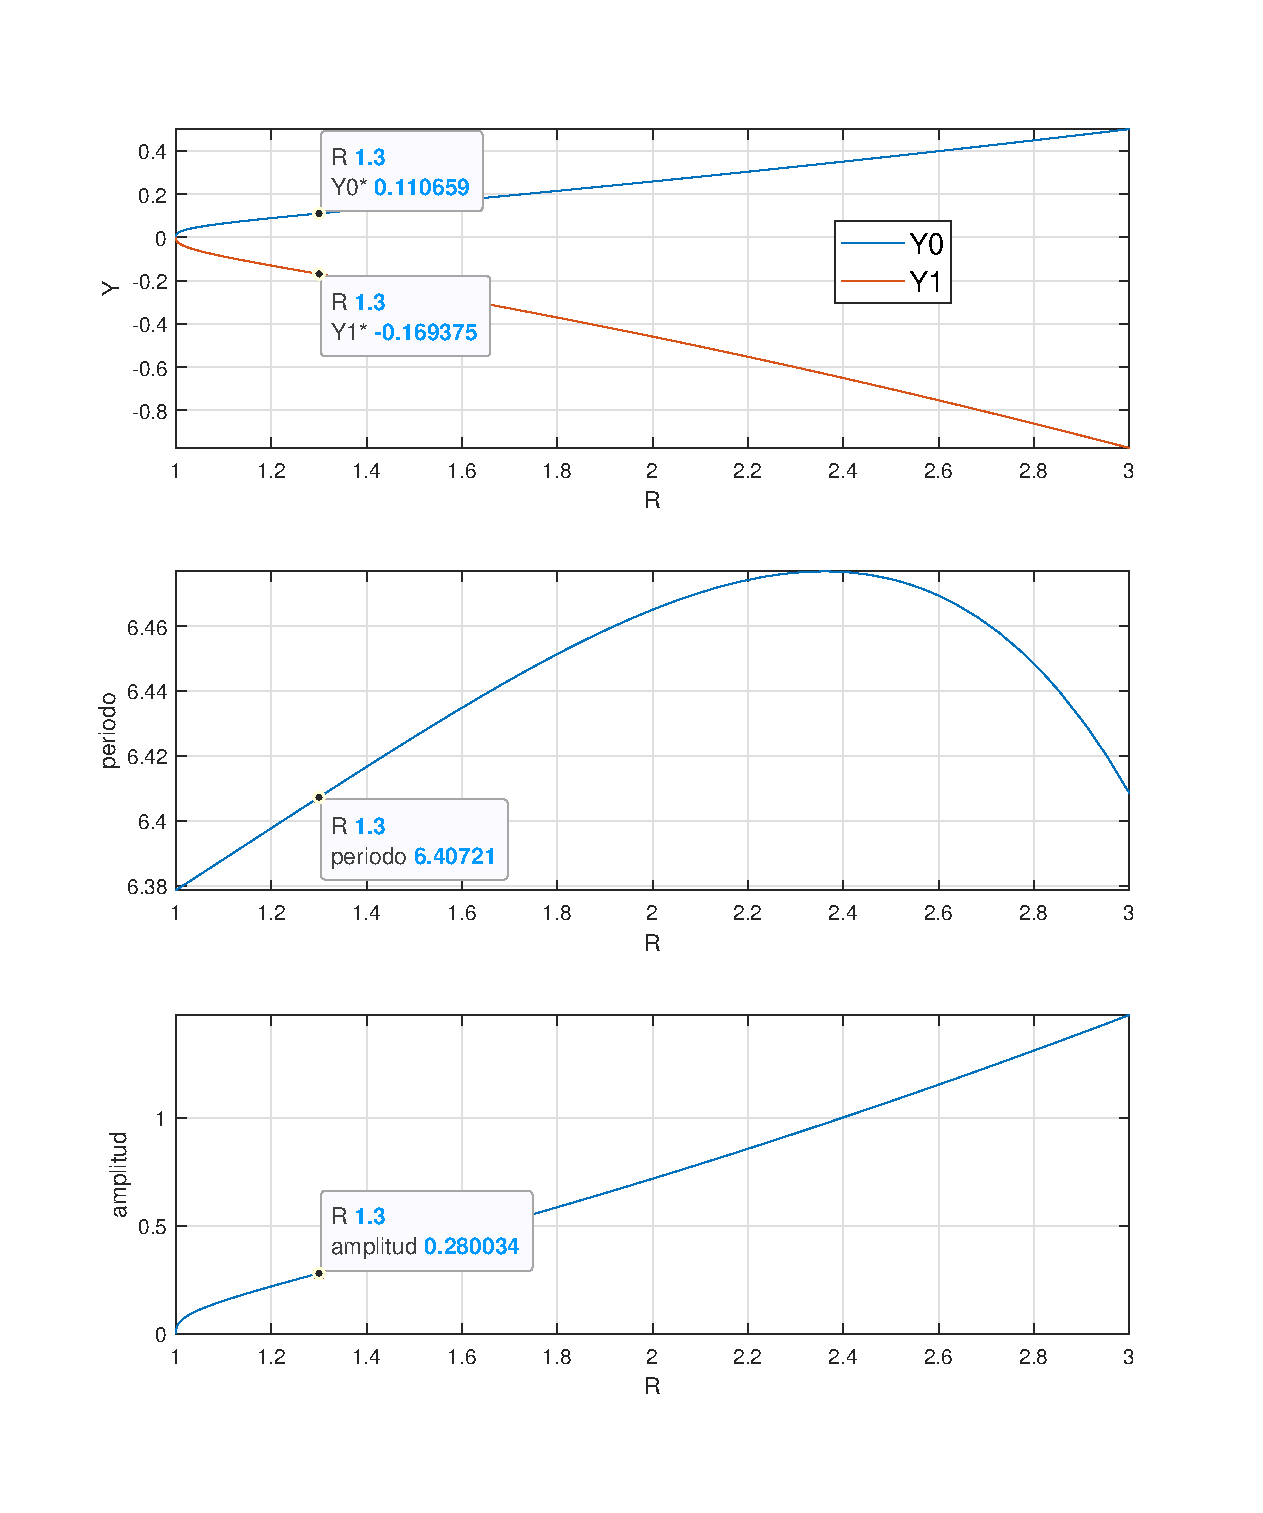
\includegraphics[width=1\textwidth]{ejem4amplitud.eps}
	\caption{Gráficas obtenidas de ``Ejemplo 4 TFE''.}
	\label{fig:ejem4}
	\end{figure}\smallskip

	\vspace{0.5cm}\noindent En la \fref{fig:ejem4} se ve la gráfica obtenida de ``Ejemplo 4 TFE'' donde aparecen la gráfica de $Y_0$ e $Y_1$ en función de $R$, la gráfica del periodo en función de $R$ y la gráfica de la amplitud también en función de $R$. Además, se muestra el punto solución $(Y_0^*,Y_1^*)$ para $R=1.3$, así como el periodo y la amplitud correspondiente.
	
	\newpage
	
	\vspace{0.5cm} A continuación veremos una pequeña modificación del código ``Ejemplo 4'' para ver más ampliamente la gráfica de $Y_0$ e $Y_1$ en función de $R$ y así comprobar que se cumplen las condiciones \eref{eq:condr} y \eref{eq:condr20}.
	
	
	\vspace{1cm}\lstinputlisting[style=Matlab-editor]{Ejemplo_5.m}
	
	\newpage
	
	\begin{figure}[h]
		\centering
		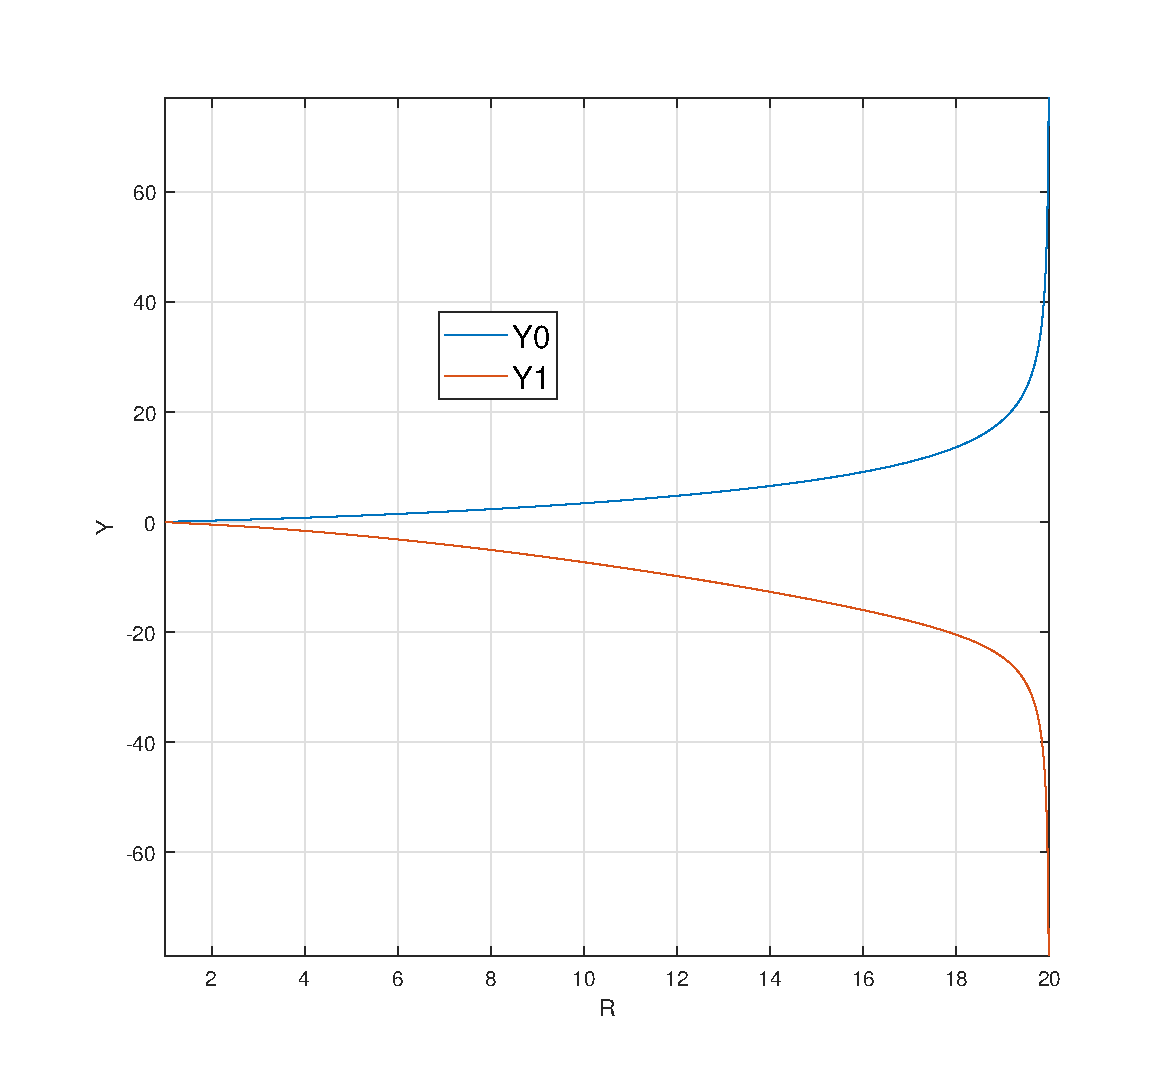
\includegraphics[width=1\textwidth]{ejem5nuevo.eps}
		\caption{Gráfica obtenida de ``Ejemplo 5''}
		\label{fig:ry1ry0}
	\end{figure}\smallskip
	
	\vspace{0.5cm}\noindent Como se puede comprobar en la \fref{fig:ry1ry0} se cumplen las condiciones \eref{eq:condr} y \eref{eq:condr20}, estas eran: $R>1$ y $R<20$ para que aparezca el ciclo límite, es decir, se empiecen a obtener valores de corte $Y_0>0$ e $Y_1<0$ con la recta de separación $X=0$.
	
	\newpage
	
	Para finalizar el estudio vamos a ver gráficamente el ciclo límite haciendo uso nuevamente de la herramienta Phase Plane, para ello hay que reescribir el sistema \eref{eq:sis2ec} como ya hicimos en \eref{eq:clejem}.
	
	\begin{equation}
		\label{eq:clejemsis}
		\scalebox{1}{$\displaystyle
			\left\{
			\begin{aligned}
				\dot{x}&=t_Ex-y+(t_C-t_E)\frac{1}{2}\left( \mid x+1 \mid - \mid x-1 \mid \right),
				\\[2mm]
				\dot{y}&=d_Ex+(d_C-d_E)\frac{1}{2}\left( \mid x+1 \mid - \mid x-1 \mid \right)-h.
			\end{aligned}
			\right. 
			$}
	\end{equation}\smallskip
	
	\vspace{0.5cm}Siendo $t_E$, $t_C$, $d_E$, $d_C$ los parámetros dados en \eref{eq:misistema}, los cuales dependen de las variables $a$, $b$, $R$, $L$, $C$ y $h$ cuyos valores se han establecido en \eref{c1f}, \eref{eq:condr}, \eref{eq:condlc} y \eref{eq:condh}. Se ha analizado el resultado para tres valores de $R$, en las siguiente figuras se presentan dichos resultados.
	
	\begin{figure}[h]
		\centering
		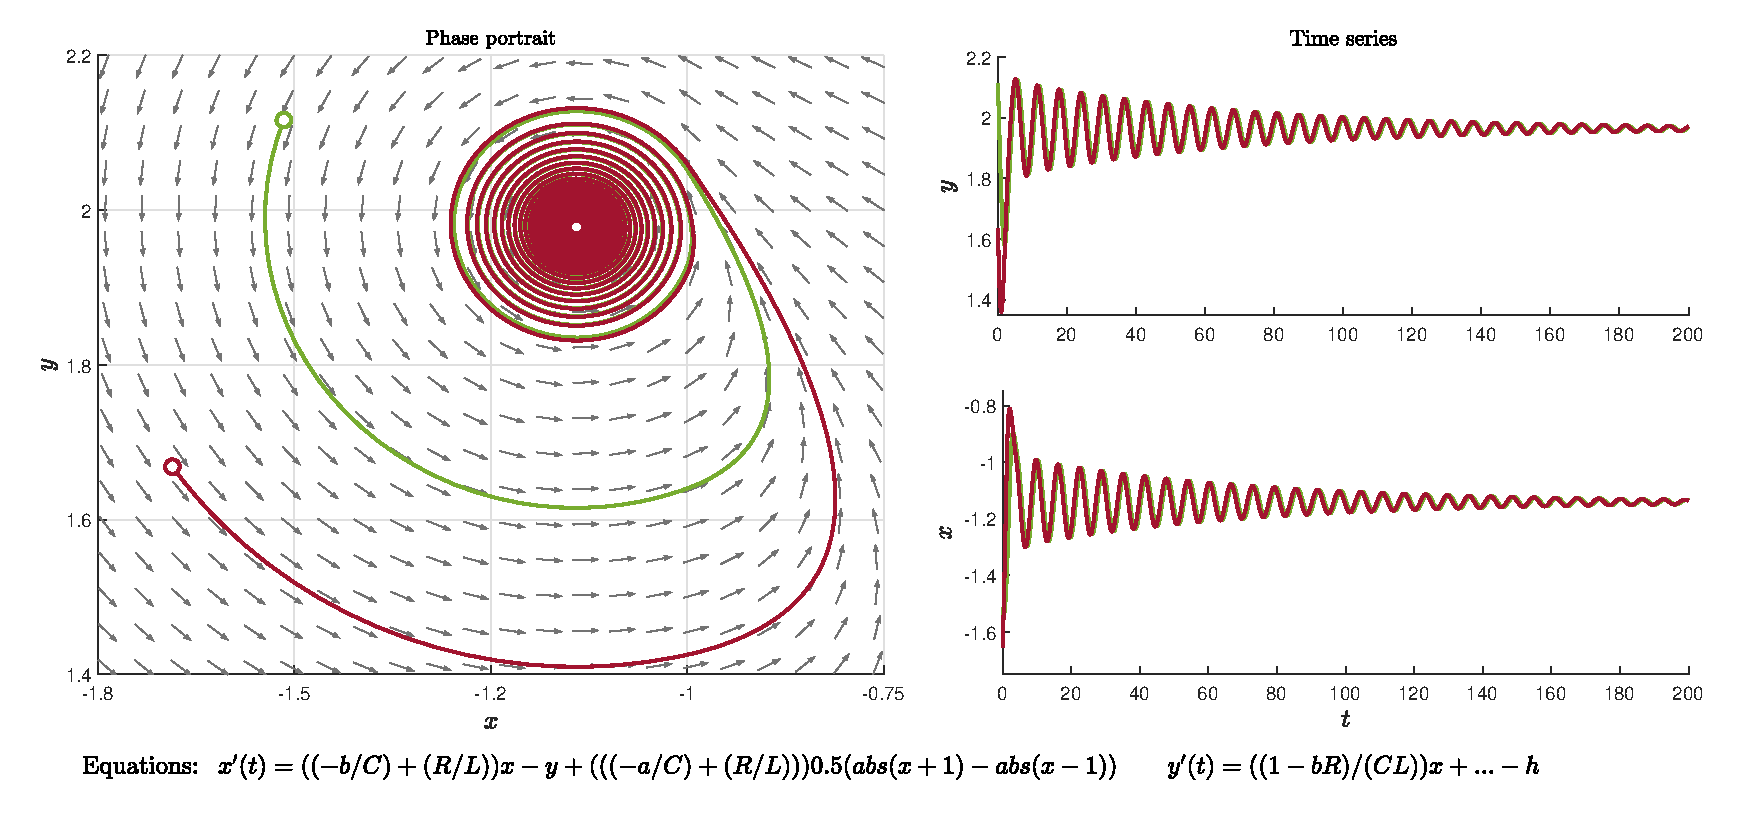
\includegraphics[width=1\textwidth]{r0.7.eps}
		\caption{Configuración de foco asintóticamente estable para $R=0.7$}
		\label{fig:r0.7}
	\end{figure}
	\begin{figure}[h]
		\centering
		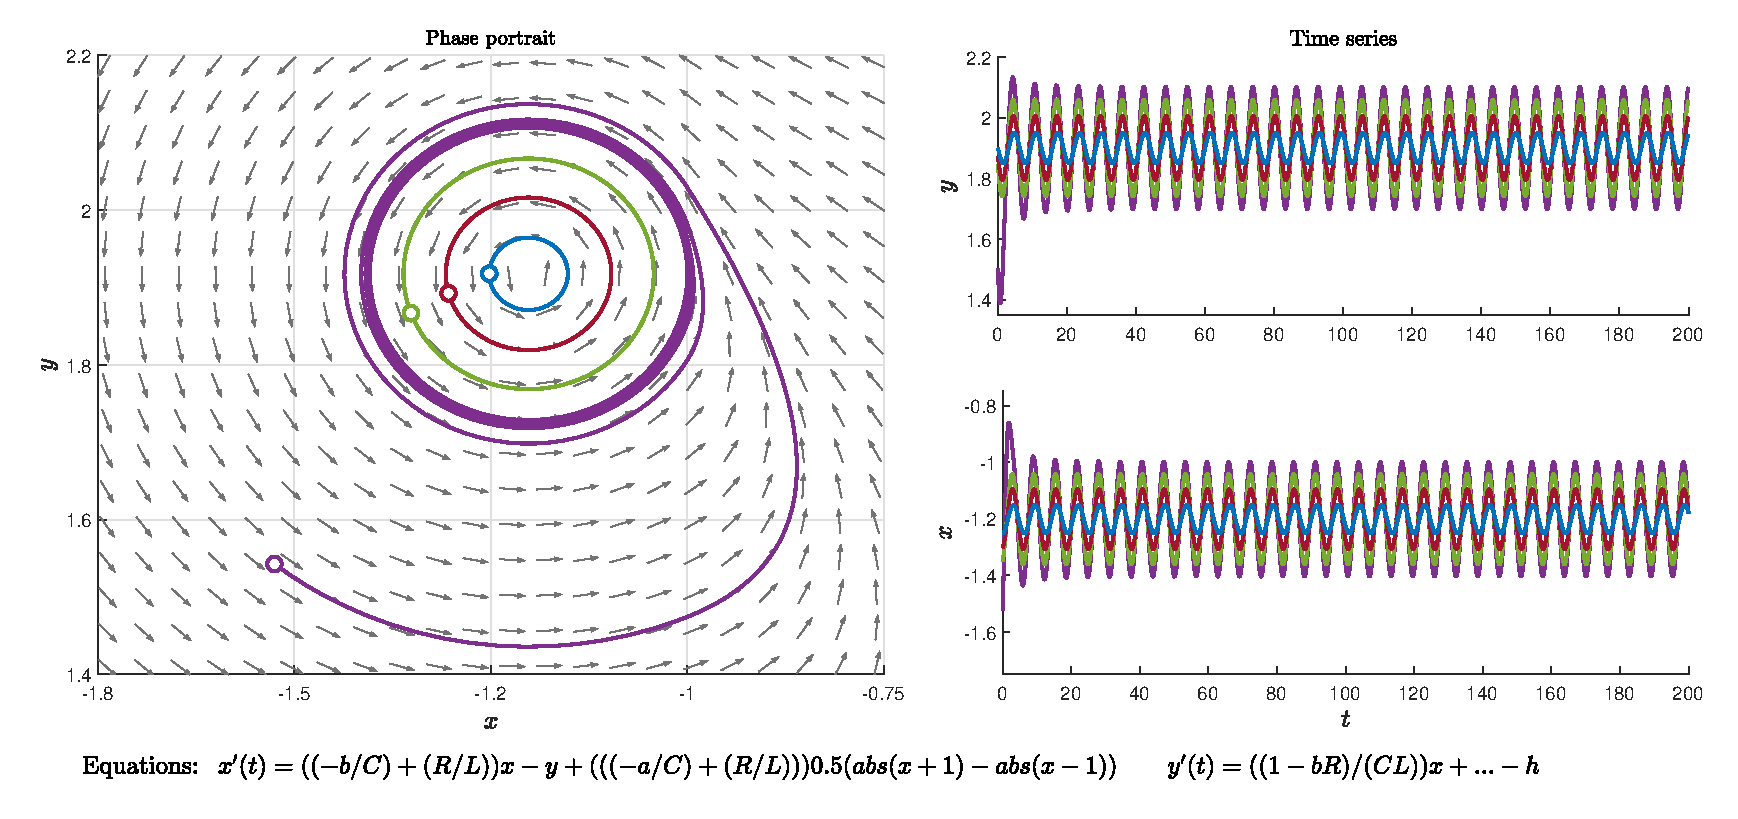
\includegraphics[width=1\textwidth]{r1.eps}
		\caption{Configuración de centro para $R=1$}
		\label{fig:r1}
	\end{figure}
	
	\newpage
	
	\begin{figure}[h]
		\centering
		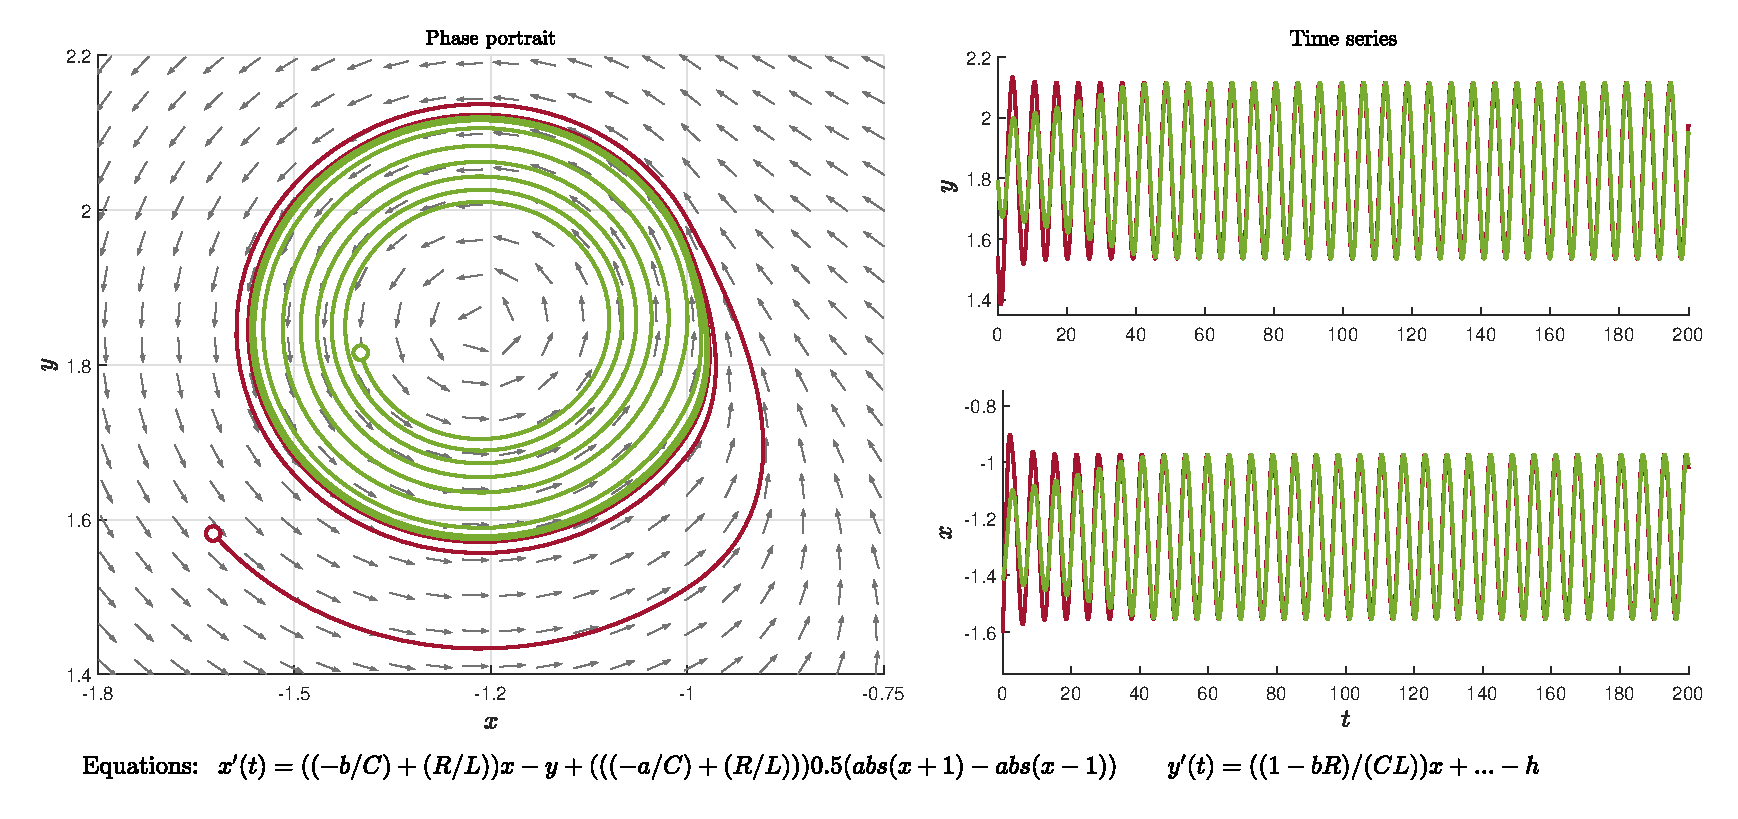
\includegraphics[width=1\textwidth]{r1.3.eps}
		\caption{Configuración de foco inestable para $R=1.3$ donde se ha producido el ciclo límite debido a la bifurcación estudiada.}
		\label{fig:r1.3}
	\end{figure}\smallskip
	
	Como se puede ver en las \fref{fig:r0.7}, \fref{fig:r1} y \fref{fig:r1.3}, hemos obtenido en nuestro circuito el mismo comportamiento que el visto en las \fref{fig:foco3}, \fref{fig:centro2} y \fref{fig:ciclolimite3}. Se puede comprobar que el ciclo límite efectivamente se introduce levemente en la zona derecha de la recta de separación, ver \fref{fig:ciclolimite3} y \fref{fig:r1.3}
	
	\vspace{0.5cm} En la herramienta Phase Plane hemos utilizado el integrador \textit{ode45} de MATLAB para resolver el sistema de ecuaciones diferenciales y así representar la solución. Ahora usaremos la función \textit{ode45} junto con la opción \textit{events} para hacer un análisis más minucioso del sistema \eref{eq:clejemsis}. Así podremos comparar los resultados que obtengamos con los que se obtuvieron previamente mediante los desarrollos en series. Haciendo uso de los \textit{events} determinaremos los puntos intersección de la órbita con la recta de separación $x=-1$ y los instantes de tiempo en los cuales se producen dichas interseccions. De esa forma podremos comprobar los puntos $y_0$ e $y_1$ además del periodo y la amplitud. Dejaremos que la función \textit{ode45} resuelva el sistema para un valor de tiempo elevado, así nos aseguraremos que los últimos valores de $y$ que cortan a al recta $x=-1$ ya están dentro del ciclo límite. En la siguiente página presentaremos el código de MATLAB utilizado para ello.
	
	\newpage
	
	\lstinputlisting[style=Matlab-editor]{Ejemplo_6.m}
	
	\vspace{0.5cm}\noindent Funciones usadas en ``Ejemplo 6'':
	\vspace{0.5cm}\lstinputlisting[style=Matlab-editor]{sistema.m}
	\vspace{0.5cm}\lstinputlisting[style=Matlab-editor]{EF.m}
	
	\newpage
	
	En el ``Ejemplo 6'', hemos seleccionado el punto inicial en $(-1,1)$. Es importante destacar que la elección del punto inicial dentro o fuera del ciclo límite no es crítica, ya que nuestro sistema con $R>1$ exhibe una configuración de ciclo límite asintóticamente estable. En consecuencia, la solución eventualmente convergerá hacia el ciclo límite, independientemente de dónde comencemos. No obstante, es esencial no seleccionar un punto inicial demasiado alejado del punto de equilibrio, ya que nuestro análisis se ha centrado en una región local y no podemos prever el comportamiento del circuito si nos alejamos significativamente del punto de equilibrio.
	
	\vspace{0.5cm}\noindent Primeramente, vamos a obtener los valores finales de la matriz xE, ya que contendrán los últimos valores de $y_0$ e $y_1$ que cruzan la recta $x=-1$. También, recordemos deshacer los cambios de variable que aplicamos anteriormente \eref{eq:cambioo1} y \eref{eq:cambioo2}.
	
	\vspace{1cm}\lstinputlisting[style=Matlab-bw]{cw1ejem6.m}
	
	\vspace{1cm}\noindent Se han obtenido unos valores de $Y_0=0.0845$ e $Y_1=-0.1141$ para $R=1.1$. Haciendo uso nuevamente del código ``Ejemplo 4'' pero esta vez para el valor $R=1.1$ se obtienen los siguientes valores
	
	\vspace{1cm}\lstinputlisting[style=Matlab-bw]{cw1ejem6_2.m}
	
	\newpage
	
	\vspace{0.5cm}\noindent A continuación comprobemos el periodo
	
	\vspace{1cm}\lstinputlisting[style=Matlab-bw]{cw2ejem6.m}
	
	\vspace{1cm}\noindent Hemos obtenido un periodo de $T_P=6.3539$, realmente parecido al obtenido en ``Ejemplo 4'', ver \fref{fig:ejem4}.
	
    \vspace{1cm}En las siguientes páginas veremos algunas gráficas interesantes que podemos generar con los resultados obtenidos de ``Ejemplo 6''.
    
    \newpage
    
    	\begin{figure}[h]
    	\centering
    	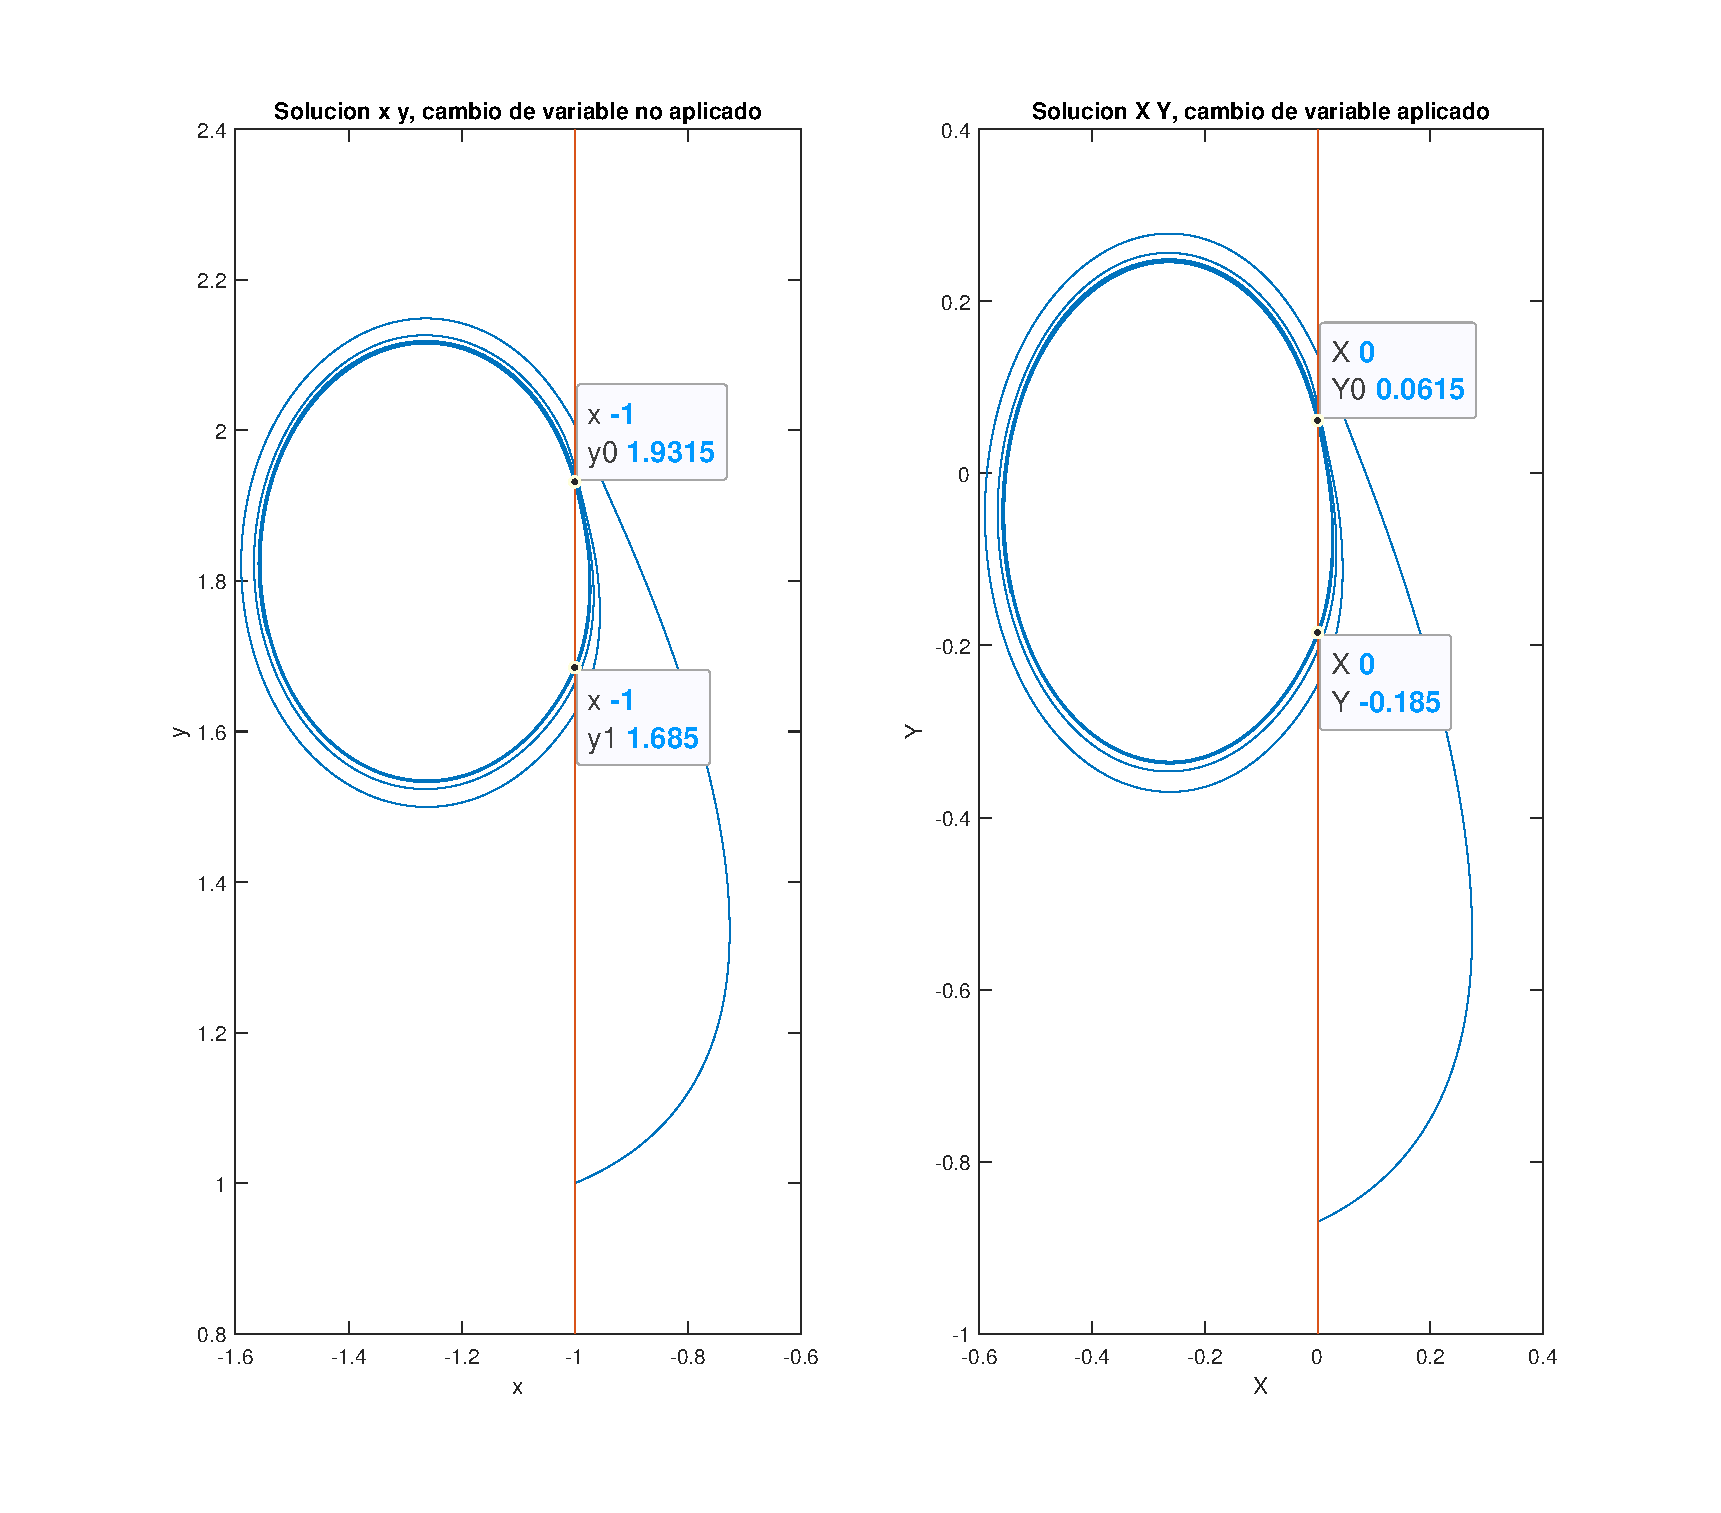
\includegraphics[width=1.2\textwidth,center]{g1ejem6tiempo.eps}
    	\caption{Comparación de la representación de la matriz \textbf{xy} de ``Ejemplo 6'' con los cambios de variable \eref{eq:cambioo1} y \eref{eq:cambioo2} aplicados y no aplicados. Los puntos representados corresponden a las dos últimas componentes de \textbf{xE}, nuevamente con cambios de variable aplicados y no aplicados.}
    	\label{fig:g1ejem6}
    \end{figure}\smallskip
    
    \vspace{0.5cm}\noindent Se han utilizado las dos últimas componentes de \textbf{xE} en la figura anterior ya que para ese valor de tiempo la órbita solución ya ha alcanzado por completo el ciclo límite.
    
    \newpage
    
    \begin{figure}[h]
    	\centering
    	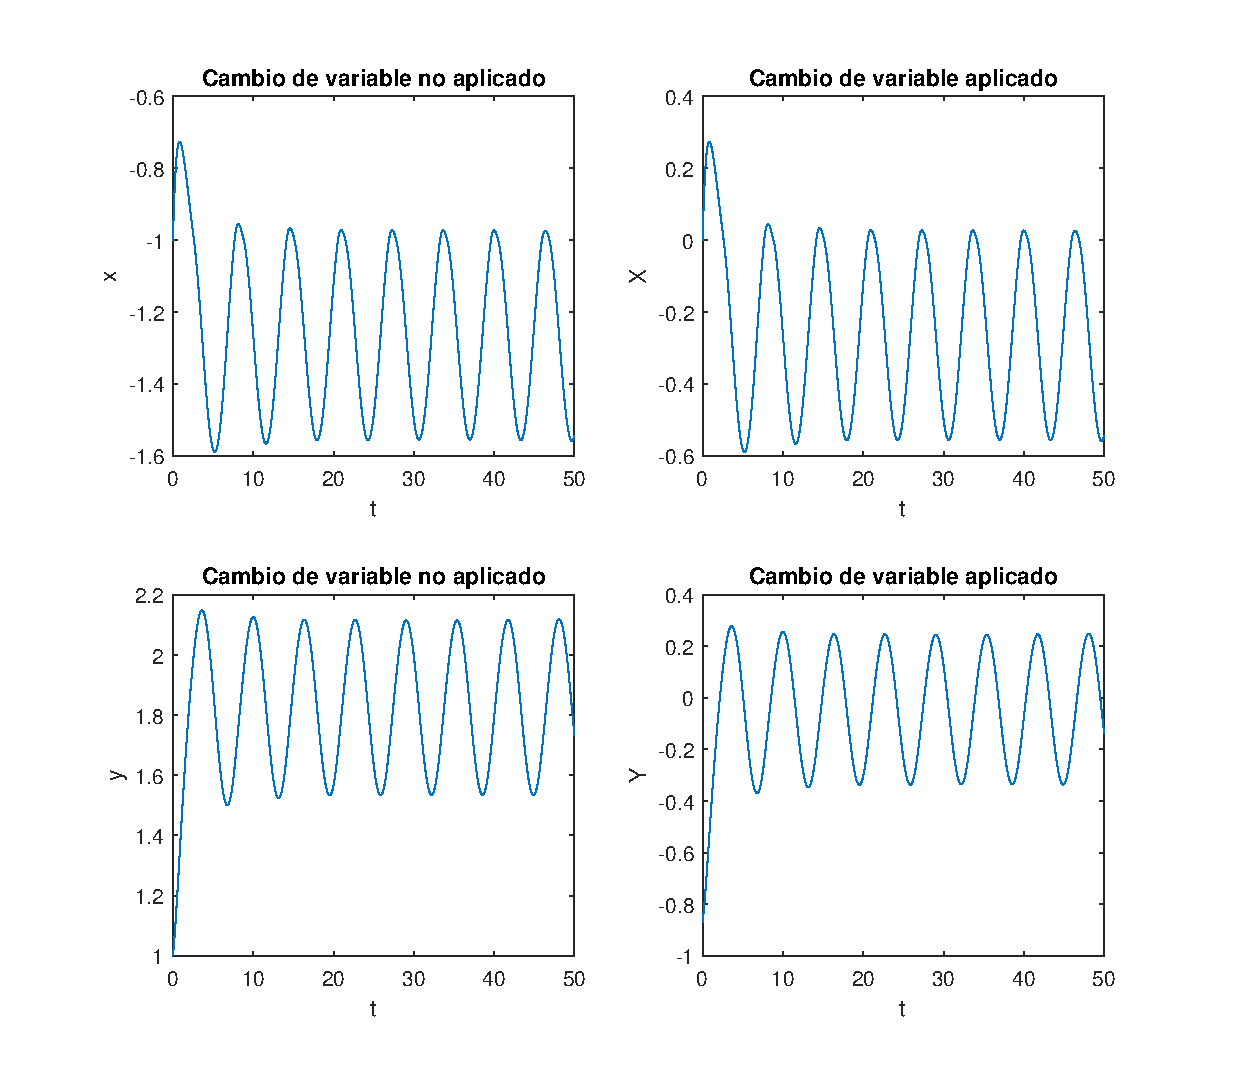
\includegraphics[width=1.2\textwidth,center]{g2ejem6tiempo.eps}
    	\caption{Comparación de la representación de las componentes de la matriz \textbf{xy} de ``Ejemplo 6'' con respecto al tiempo de estudio \textbf{t} con los cambios de variable \eref{eq:cambioo1} y \eref{eq:cambioo2} aplicados y no aplicados}
    	\label{fig:g2ejem6}
    \end{figure}\smallskip
	
	\newpage
	
	\begin{figure}[h]
		\centering
		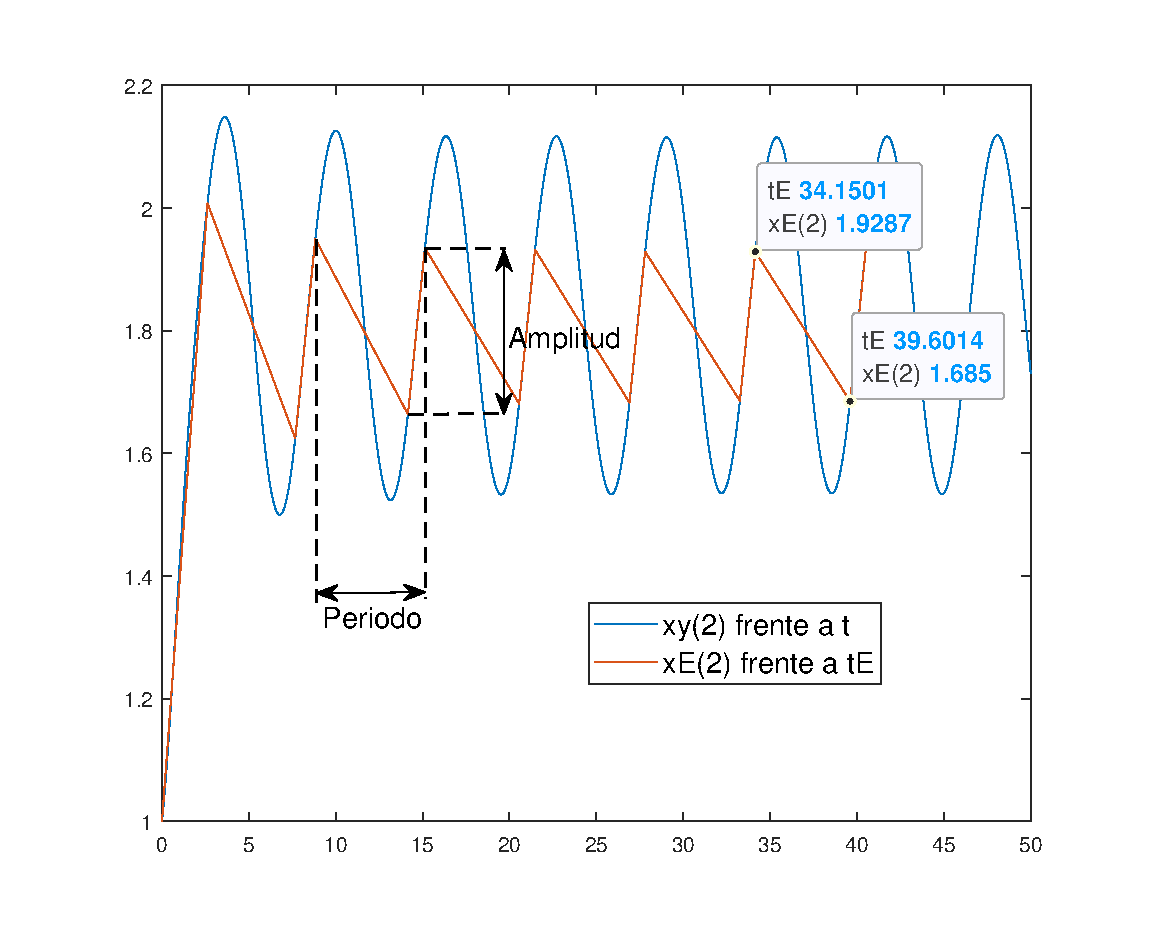
\includegraphics[width=1.1\textwidth,center]{g3ejem6tiempo.eps}
		\caption{Comparación de las gráficas de \textbf{y (xy(2))} solución frente al tiempo de estudio \textit{\textbf{t}} y los valores de \textbf{y (xE(2))} para los que se produce el evento de corte con la recta $x=-1$ frente a los instantes de tiempo \textbf{tE} en que se produce el evento.}
		\label{fig:g3ejem6}
	\end{figure}\smallskip
	
	\vspace{0.5cm} La \fref{fig:g3ejem6} resulta especialmente interesante, ya que proporciona una visualización clara de los puntos de intersección $y_0$ e $y_1$, así como de la manera en que se pueden medir tanto el periodo como la amplitud de la oscilación.
	
	\vspace{0.5cm} Las gráficas previamente presentadas se generaron utilizando ``Graficas Ejemplo 6", cuyo código se encuentra detallado en la siguiente página.
	
	\newpage
	
	\vspace{0.5cm}\lstinputlisting[style=Matlab-editor]{Graficas_Ejemplo_6.m}
	
	\newpage
	
	El próximo y último paso de este trabajo consistirá en regresar a las ecuaciones originales del circuito \eref{eq:sistema} y verificar de manera efectiva la existencia de dicho ciclo límite, con una condición inicial $(x_0,y_0,z_0)$. Para lograrlo, deberemos revertir todas los cambios de variable que hemos aplicado a lo largo del estudio. 
	
	\vspace{0.5cm}Si examinamos el sistema \eref{eq:cb3}, es evidente que dado que el ciclo límite es asintóticamente estable, y basándonos en la gráfica derecha de la \fref{fig:g1ejem6},  si seleccionamos el punto inicial $(X_0, Y_0) = (0, 0)$, la solución del sistema tenderá hacia el ciclo límite cuando pase el suficiente tiempo. Por esta razón, hemos optado por tomar el punto $(X_0, Y_0) = (0, 0)$ como punto de partida para el proceso de deshacer las transformaciones y determinar así las condiciones iniciales adecuadas para el circuito.
	
	\vspace{0.5cm}\noindent El siguiente paso es deshacer los cambios de variable \eref{eq:cambioo1} y \eref{eq:cambioo2}:
	
	\begin{equation}
		\label{eq:desh1}
		\begin{gathered}
			(x_0,y_0)=\left( X_0-1,Y_0-t_c \right) = (0-1,0-t_C) \\[5mm]
			(x_0,y_0)=(-1,-t_C)
		\end{gathered}
	\end{equation}\smallskip
	
	
		\vspace{0.5cm} Las condiciones iniciales \eref{eq:desh1} corresponden al sistema ``bizonal'' \eref{eq:sisbiz}. Como ya se comentó, este sistema no es mas que una simplificación del sistema \eref{eq:sis2ec}, por lo que la conversión de las condiciones iniciales anteriores es directa:	
	
	\begin{equation}
		\label{eq:desh2}
		(\tilde{x_0},\tilde{y_0}) = (-1,-t_C)
	\end{equation}\smallskip
	
	En última instancia, debemos proceder a deshacer las transformaciones de variable que se llevaron a cabo para pasar del sistema tridimensional \eref{eq:sistema} al sistema bidimensional \eref{eq:sis2ec}. Esta tarea ya ha sido preparada en las ecuaciones \eref{eq:solsis}, de manera que ahora solo debemos realizar la sustitución de los valores $\tilde{x_0}$, $\tilde{y_0}$ y $h_0$, teniendo en cuenta que previamente se estableció $h = h_0=-1$. De este modo, obtendremos:
	
\begin{subequations}
	\label{eq:deshh}
	\begin{align}
		z_0=&\tilde{x_0}=-1. \label{eq:desh3} \\[5mm]
		y_0=& \frac{\alpha_1\tilde{x_0}+\frac{h_0}{a_{22}}-\tilde{y_0}}{\alpha_3} = \frac{\alpha_1(-1)+\frac{(-1)}{a_{22}}-(-t_C)}{\alpha_3} = \frac{-\alpha_1-\frac{1}{a_{22}}+t_C}{\alpha_3} \label{eq:desh4}. \\[5mm]
		x_0= &\frac{a_{12}}{a_{22}}y_0+a_{11}q(\tilde{x_0})-\frac{a_{12}a_{21}}{a_{22}}\tilde{x_0}-\frac{h_0}{a_{22}}=\notag\\[3mm] &\frac{a_{12}}{a_{22}}  \left( \frac{-\alpha_1-\frac{1}{a_{22}}+t_C}{\alpha_3} \right)+a_{11}q(-1)-\frac{a_{12}a_{21}}{a_{22}}(-1)-\frac{-1}{a_{22}}=\notag\\[3mm]
		&\frac{a_{12}}{a_{22}}  \left( \frac{-\alpha_1-\frac{1}{a_{22}}+t_C}{\alpha_3} \right)+a_{11}q(-1)+\frac{a_{12}a_{21}}{a_{22}}+\frac{1}{a_{22}}. \label{eq:desh5}
	\end{align}
\end{subequations}

\newpage

	\noindent Los valores anteriores se calcularán haciendo uso del siguiente código
	
	\vspace{0.5cm}\lstinputlisting[style=Matlab-editor]{Condiciones_Iniciales.m}
	
	\vspace{1cm}\lstinputlisting[style=Matlab-bw]{condicionesiniciales.m}
	
	\newpage
	
	\noindent Recordemos que las variables de estado son:
	\begin{itemize}
		\item $x(t)$ es la tensión ($v_1$) en el condensador y el memristor.
		\item $y(t)$ es la intensidad ($i_{LR}$) en la resistencia y la bobina.
		\item $z(t)$ es el flujo ($\varphi$) en el memristor.
	\end{itemize}
	
	\vspace{0.4cm}\noindent Por lo que aplicando una tensión inicial $v_1=-1.7764\cdotp 10^{-15} \simeq 0 (\text{v})$ y una intensidad inicial $i_{LR}=-0.02=-20(\text{mA})$ aparecerá el ciclo limite asintóticamente estable en el circuito. Vamos a comprobarlo haciendo uso de la función \textit{ode45} como hicimos anteriormente en ``Ejemplo 6''.
	
	\vspace{0.5cm}\lstinputlisting[style=Matlab-editor]{Ejemplo_6_Tridimensional.m}
	
	\vspace{0.5cm}\noindent Función usada en ``Ejemplo 6 Tridimensional'':
	\vspace{0.5cm}\lstinputlisting[style=Matlab-editor]{sistematridi.m}
	
	\newpage
	
	 Utilizando el código ``Ejemplo 6 Tridimensional'', obtendremos los valores $x$, $y$, $z$ como resultado de la integración del sistema \eref{eq:sistema}. Además, variaremos manualmente el valor de $R$ en la función ``sistematridi'' con los siguientes tres valores $R=0.7$, $R=1$ y $R=1.3$, lo que nos permitirá visualizar la bifurcación foco-centro-ciclo límite, tal como se ha explicado previamente. A continuación, presentaremos el código "Bifurcacion Planos 1", el cual se utiliza para representar en 3D los resultados obtenidos.
	
	\vspace{0.5cm}\lstinputlisting[style=Matlab-editor]{Bifurcacion_Planos_1.m}
	
	\newpage
	
	\begin{figure}[h]
		\centering
		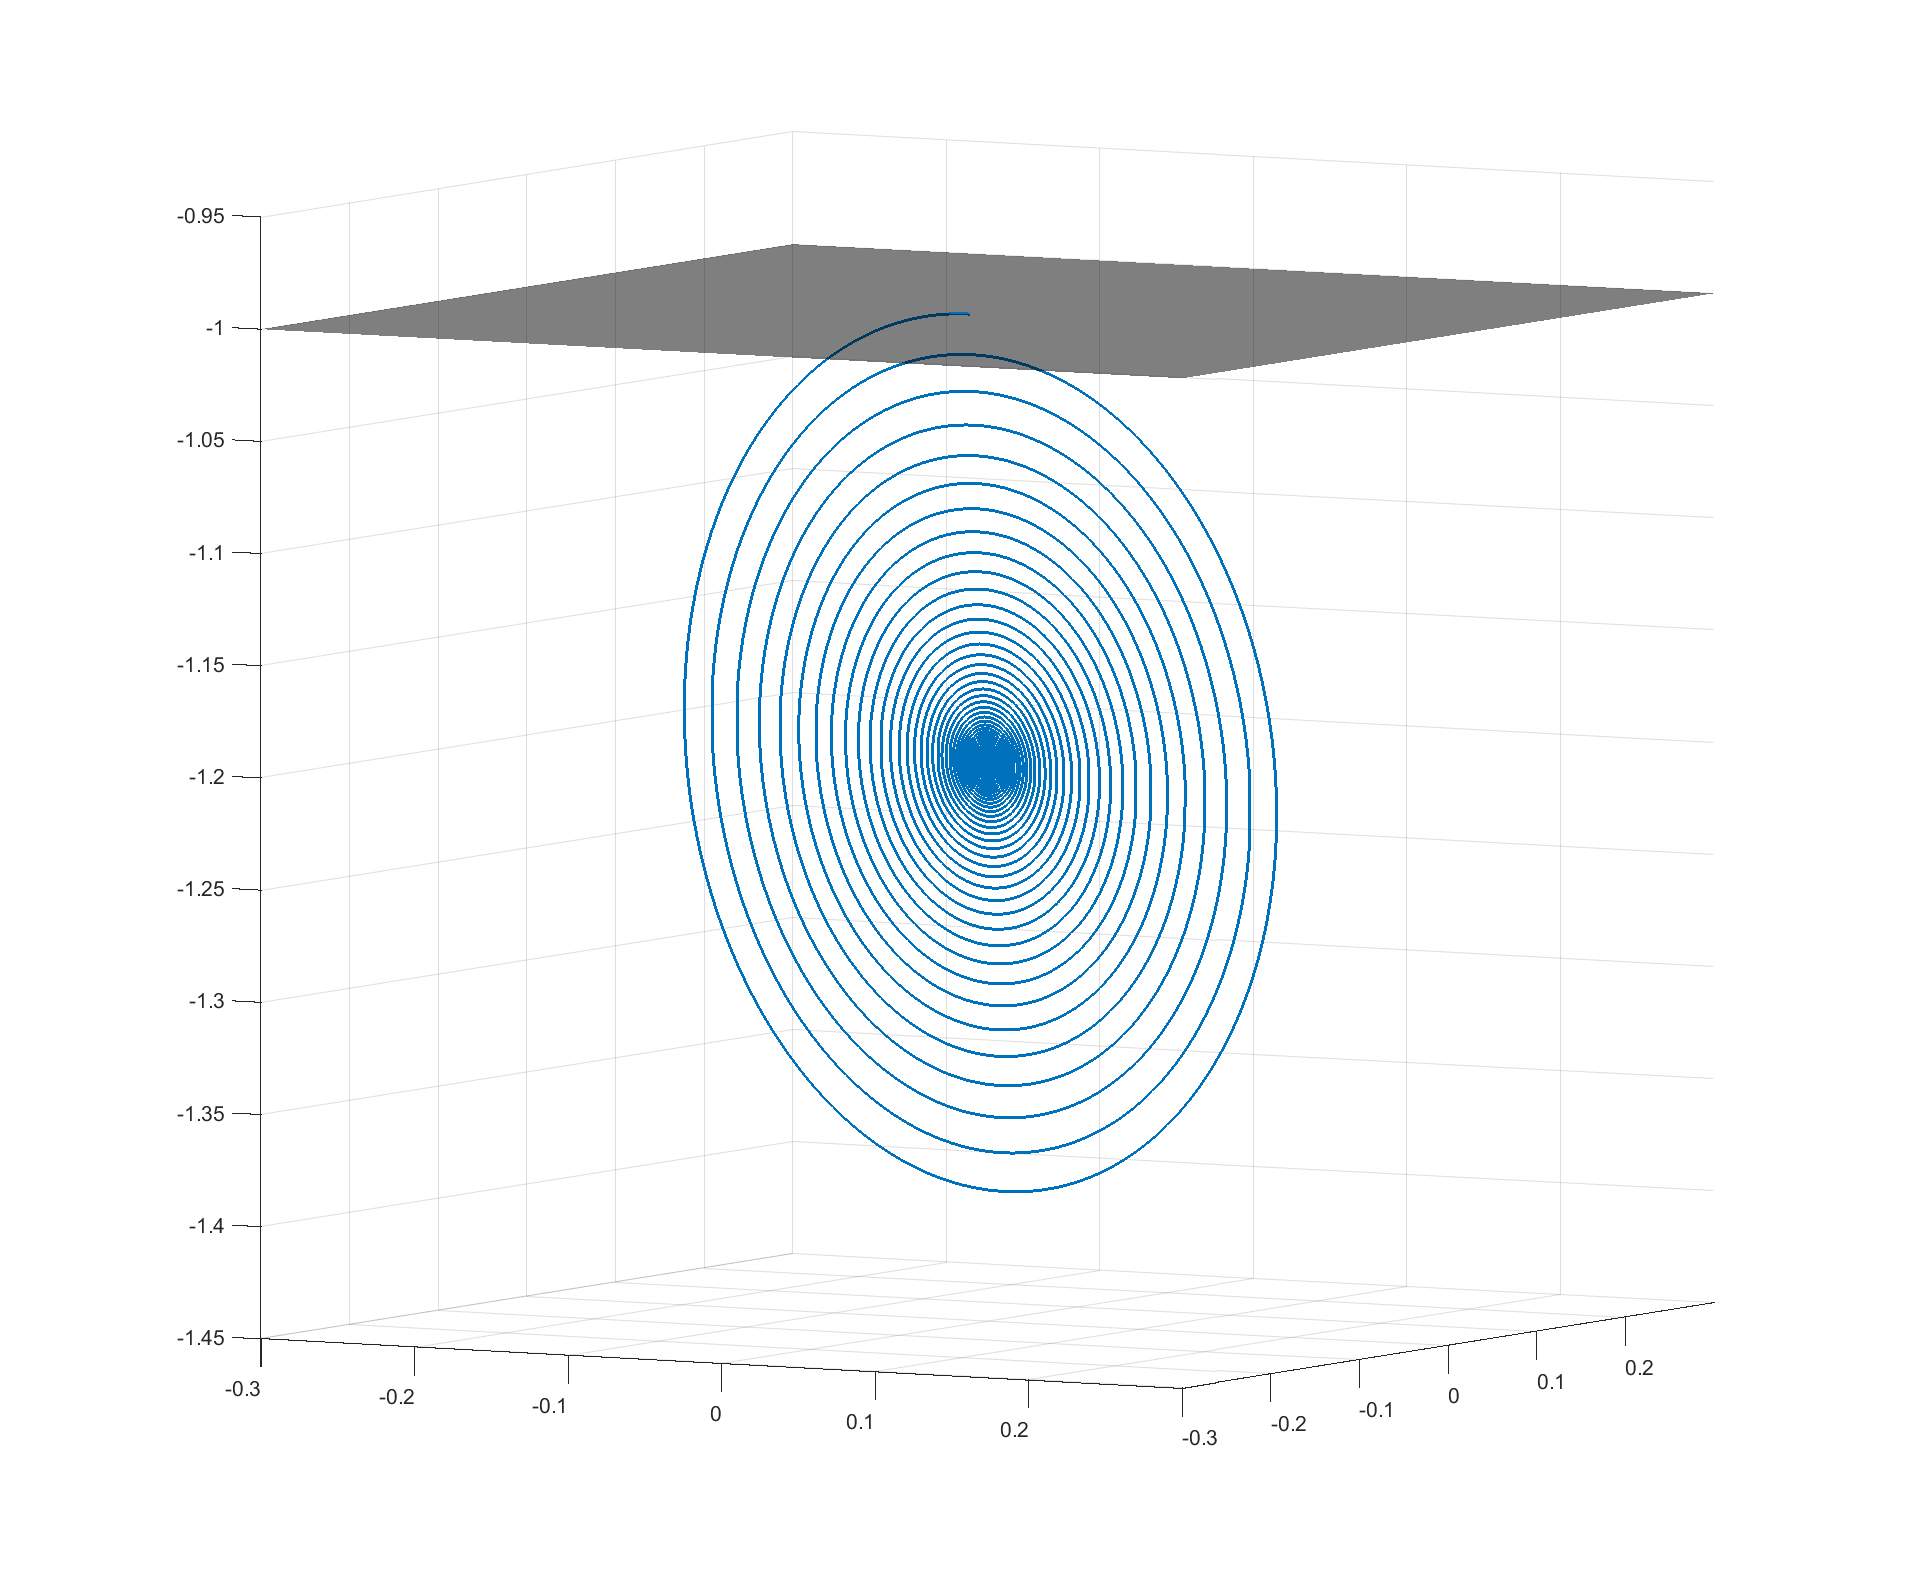
\includegraphics[width=1\textwidth]{fococir.eps}
		\caption{Gráfica resultado de ``Bifurcacion Planos 1'' para un valor de $R=0.7$ en ``sistematridi''.}
		\label{fig:fococircuito}
	\end{figure}\smallskip
	
	\vspace{0.5cm}\noindent En la \fref{fig:fococircuito}, se aprecia la configuración de foco asintóticamente estable para un valor de $R<1$ en el sistema \eref{eq:sistema}, utilizando las condiciones iniciales previamente calculadas.
	
	\newpage
	
	\begin{figure}[h]
		\centering
		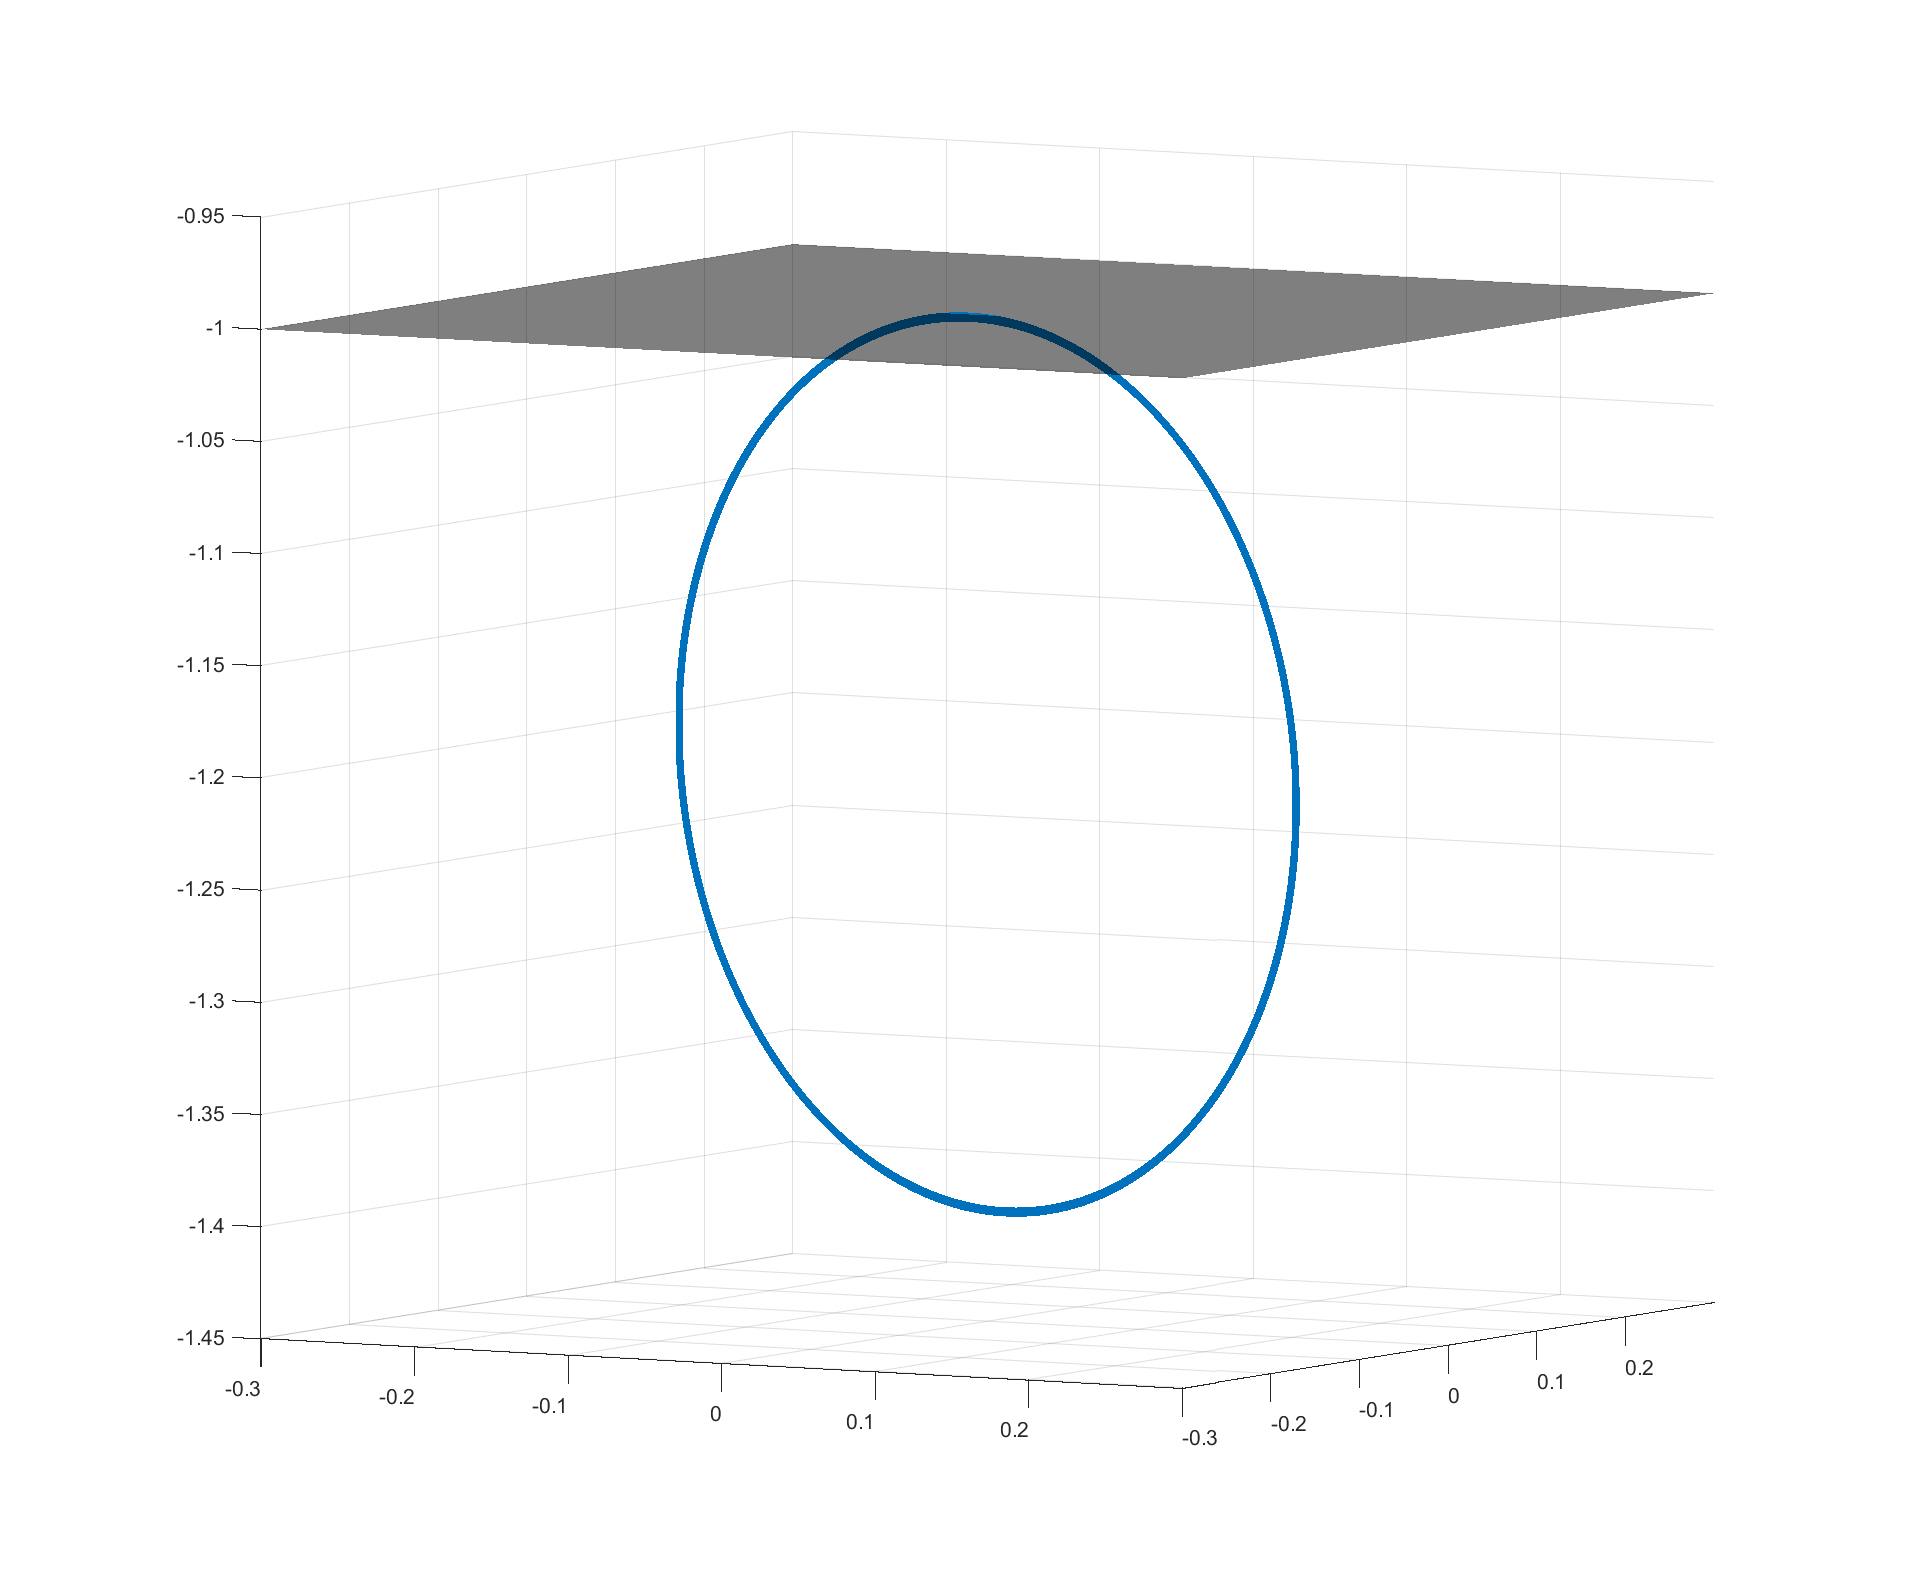
\includegraphics[width=1\textwidth]{centrocir.eps}
		\caption{Gráfica resultado de ``Bifurcacion Planos 1'' para un valor de $R=1$ en ``sistematridi''.}
		\label{fig:centrocircuito}
	\end{figure}\smallskip
	
		\vspace{0.5cm}\noindent En la \fref{fig:centrocircuito}, se observa la configuración de centro para un valor de $R=1$ en el sistema \eref{eq:sistema}, utilizando las condiciones iniciales previamente calculadas. Se puede notar que la última órbita es tangente a la superficie de separación, y será precisamente de esta órbita de donde surgirá el ciclo límite.
	
	\newpage
	
	\begin{figure}[h]
		\centering
		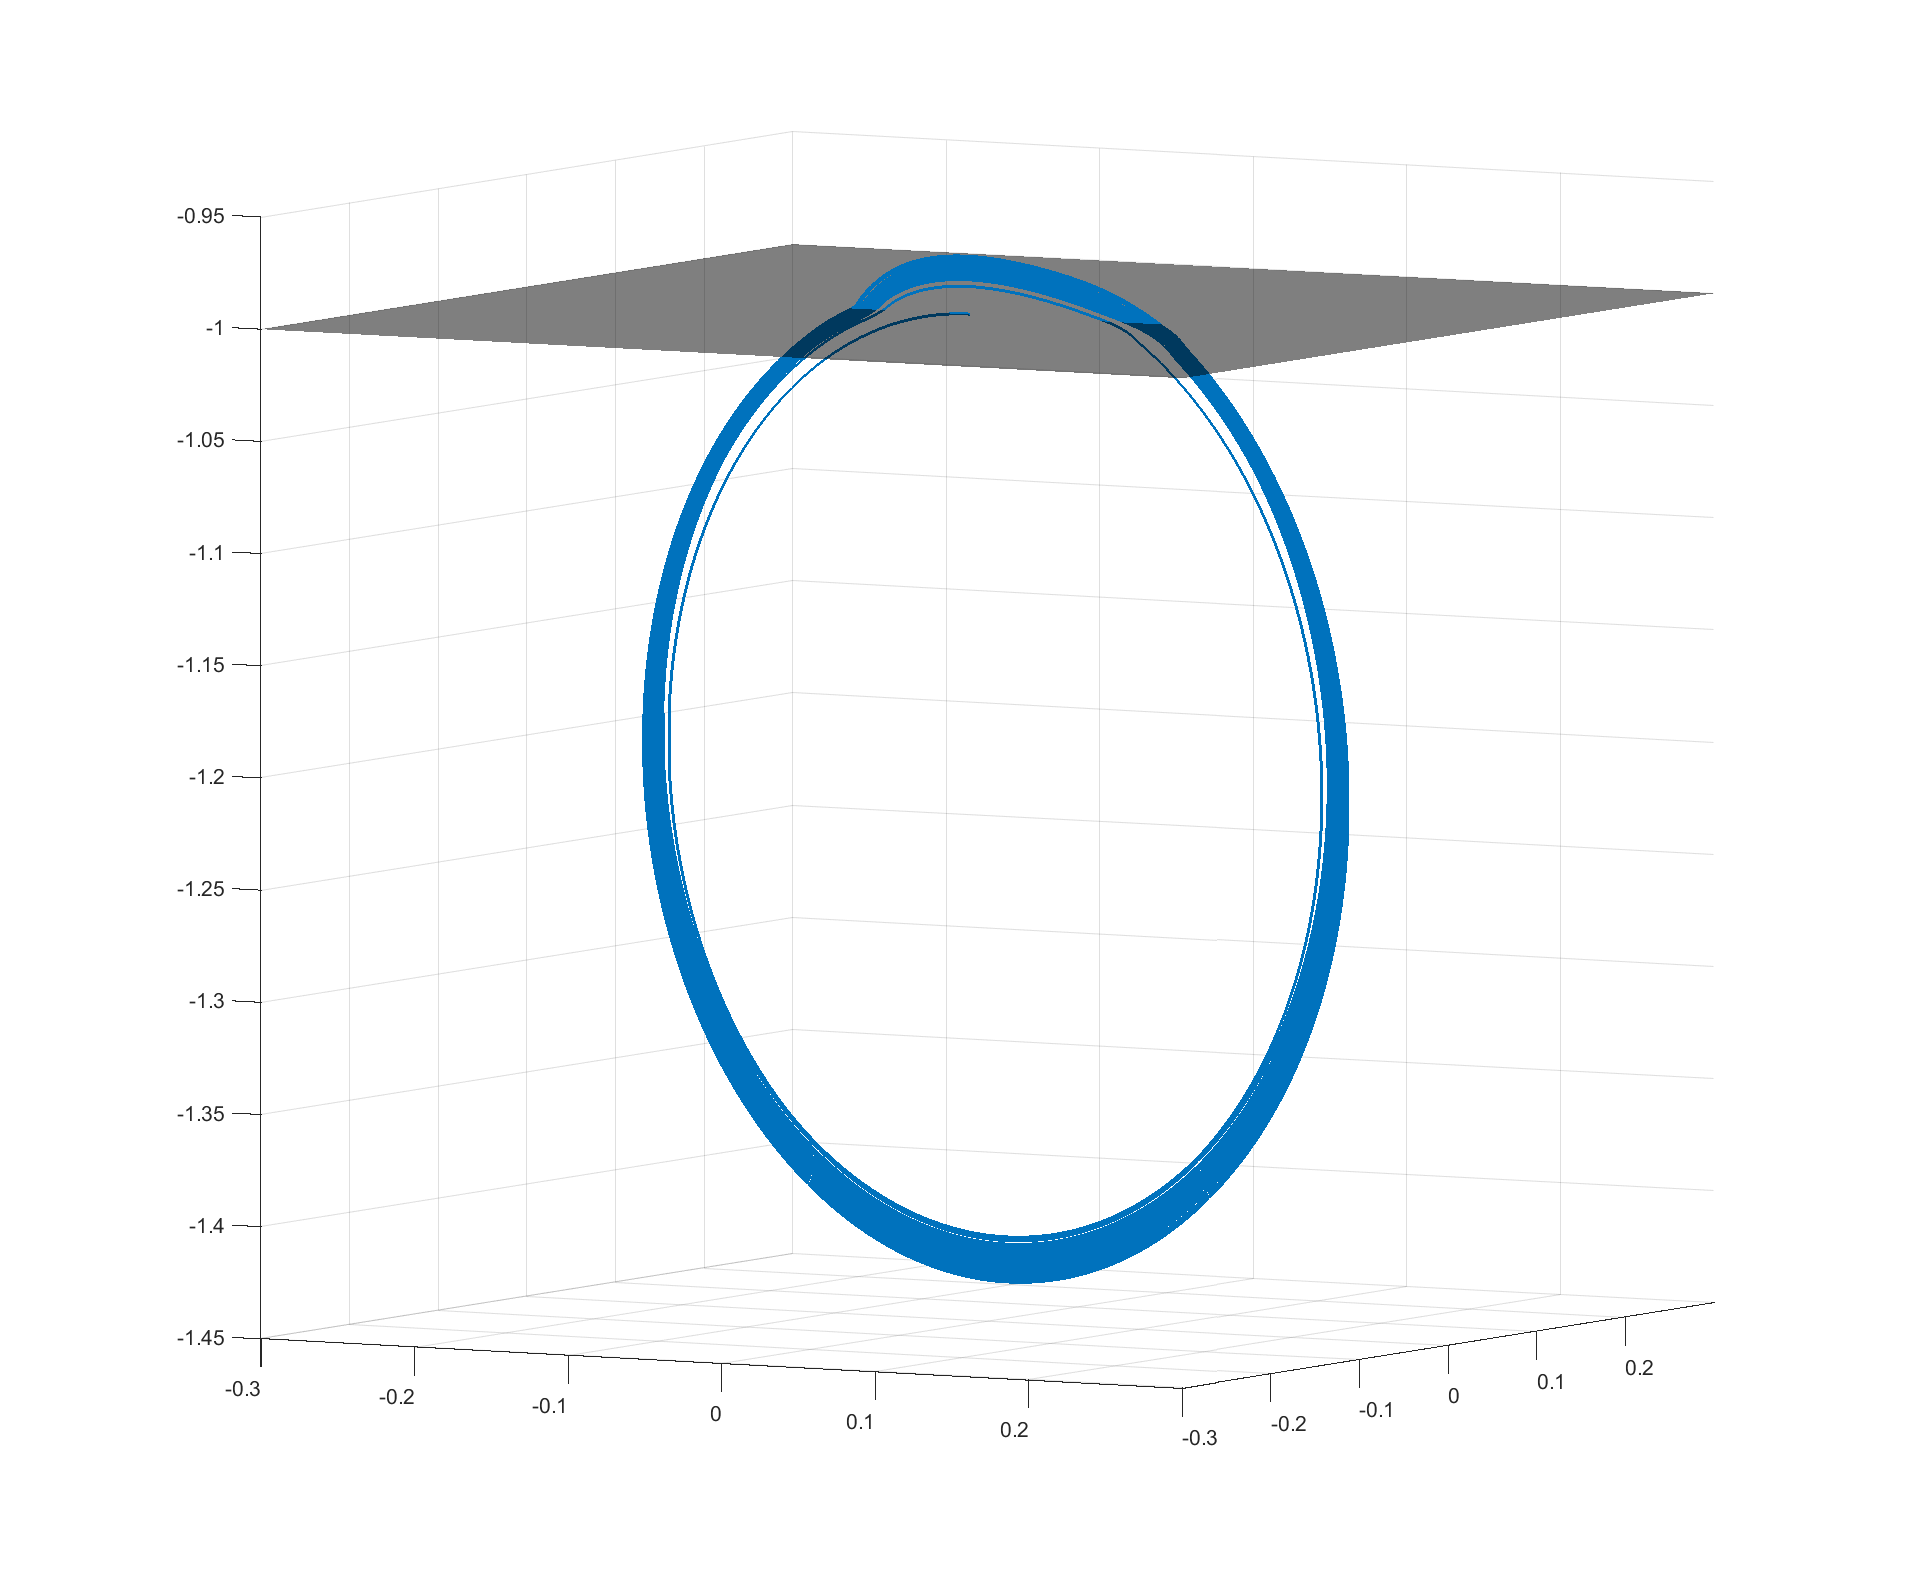
\includegraphics[width=1\textwidth]{ciclocir.eps}
		\caption{Gráfica resultado de ``Bifurcacion Planos 1'' para un valor de $R=1.3$ en ``sistematridi''.}
		\label{fig:ciclocircuito}
	\end{figure}\smallskip
	
		\vspace{0.5cm}\noindent En la \fref{fig:ciclocircuito}, se representa la configuración de ciclo límite asintóticamente estable para un valor de $R>1$ en el sistema \eref{eq:sistema}, utilizando las condiciones iniciales previamente calculadas. Se puede observar cómo el ciclo límite efectivamente se introduce en la zona adyacente levemente.
		
		\newpage
		
	Aunque en la \fref{fig:ciclocircuito} no sea muy evidente, las dos partes del ciclo límite, tanto en la zona superior como en la inferior del plano de separación, están contenidas en planos distintos (recordar que la dinámica del sistema es bidimensional). A continuación obtendremos la expresión de ambos planos para representarlos y ver dicha diferencia, basta con despejar $z$ de la ecuación \eref{eq:hecuation}, sustituyendo \eref{eq:qf}:
		
		\begin{subequations}
			\label{eq:funcz}
			\begin{align}
				\text{Para}\; z<-1 \quad \rightarrow \quad h_0&=-a_{22}x+a_{12}y-a_{12}a_{21}z+a_{11}a_{22}(b(z+1)-a),\notag\\[3mm]
				z&=-\frac{h_0+a_{22}x-a_{12}y+a_{11}a_{22}(a-b)}{a_{12}a_{21}-a_{11}a_{22}b}=:z_1. \label{eq:z1} \\[5mm]
				\text{Para}\; z>-1 \quad \rightarrow \quad h_0&=-a_{22}x+a_{12}y-a_{12}a_{21}z+a_{11}a_{22}(az),\notag\\[3mm]
				z&=-\frac{h_0+a_{22}x-a_{12}y}{a_{12}a_{21}-a_{11}a_{22}a}=:z_2. \label{eq:z2}
			\end{align}
		\end{subequations}
		
	\vspace{0.5cm}Seguidamente, presentaremos el código utilizado para representar ambos planos $z_1$ y $z_2$, lo que nos permitirá observar con mayor claridad que, efectivamente, no son el mismo.
	
	\vspace{0.5cm}\lstinputlisting[style=Matlab-editor]{Bifurcacion_Planos_2.m}
	
	\newpage
	
	\begin{figure}[h]
		\centering
		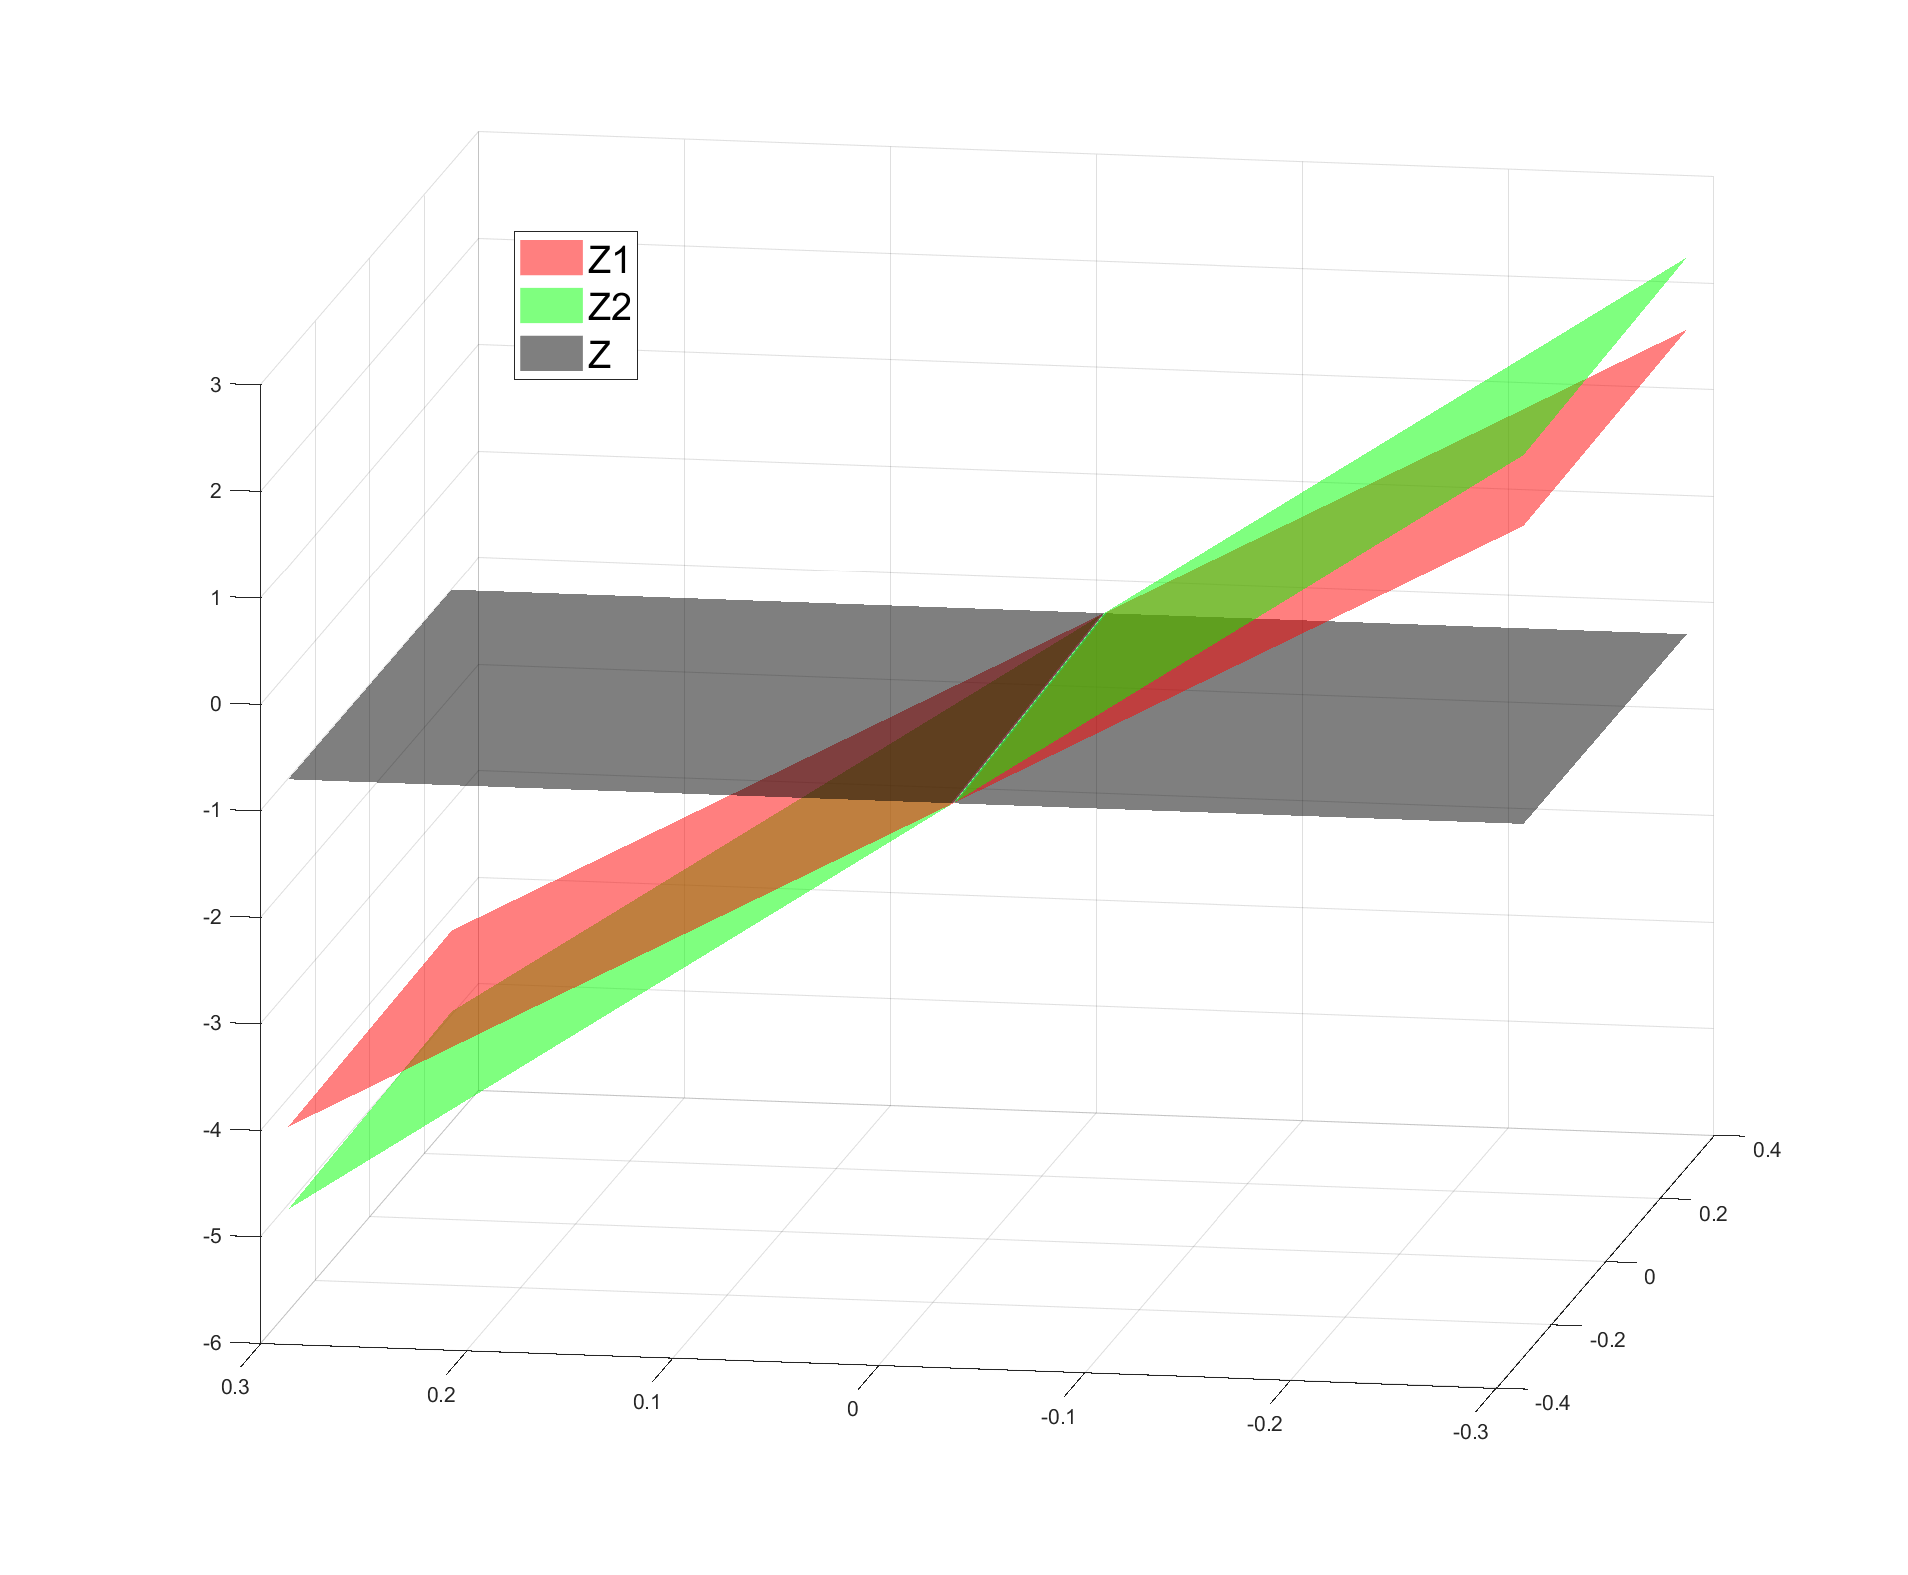
\includegraphics[width=1\textwidth]{planoscircuito.eps}
		\caption{Gráfica resultado de ``Bifurcacion Planos 2''.}
		\label{fig:planoscircuito}
	\end{figure}\smallskip
	
	\vspace{0.5cm} En la \fref{fig:planoscircuito}, se ve la representación del plano $z_1$ (rojo) que contendrá la porción mayor de ciclo límite y el plano $z_2$ (verde) que contendrá la pequeña porción de ciclo límite que traspasará el plano de separación $\tilde{x}=-1$. Por último, presentaremos una figura que compara las tres figuras anteriores (\fref{fig:fococircuito}, \fref{fig:centrocircuito}, \fref{fig:ciclocircuito}) junto con los planos de la \fref{fig:planoscircuito}. Para ello, utilizaremos ``Bifurcacion Planos 3'' para generar las figuras, que se guardarán manualmente con los nombres `foco25.fig', `centro25.fig' y `ciclo25.fig', posteriormente las combinaremos utilizando ``Bifurcacion Combinar Planos''.
	\newpage
	
	\vspace{0.5cm}\lstinputlisting[style=Matlab-editor]{Bifurcacion_Planos_3.m}
	
	\newpage
	
	\vspace{0.5cm}\lstinputlisting[style=Matlab-editor]{Bifurcacion_Combinar_Planos.m}
	
	\newpage
	
	\begin{figure}[h]
		\centering
		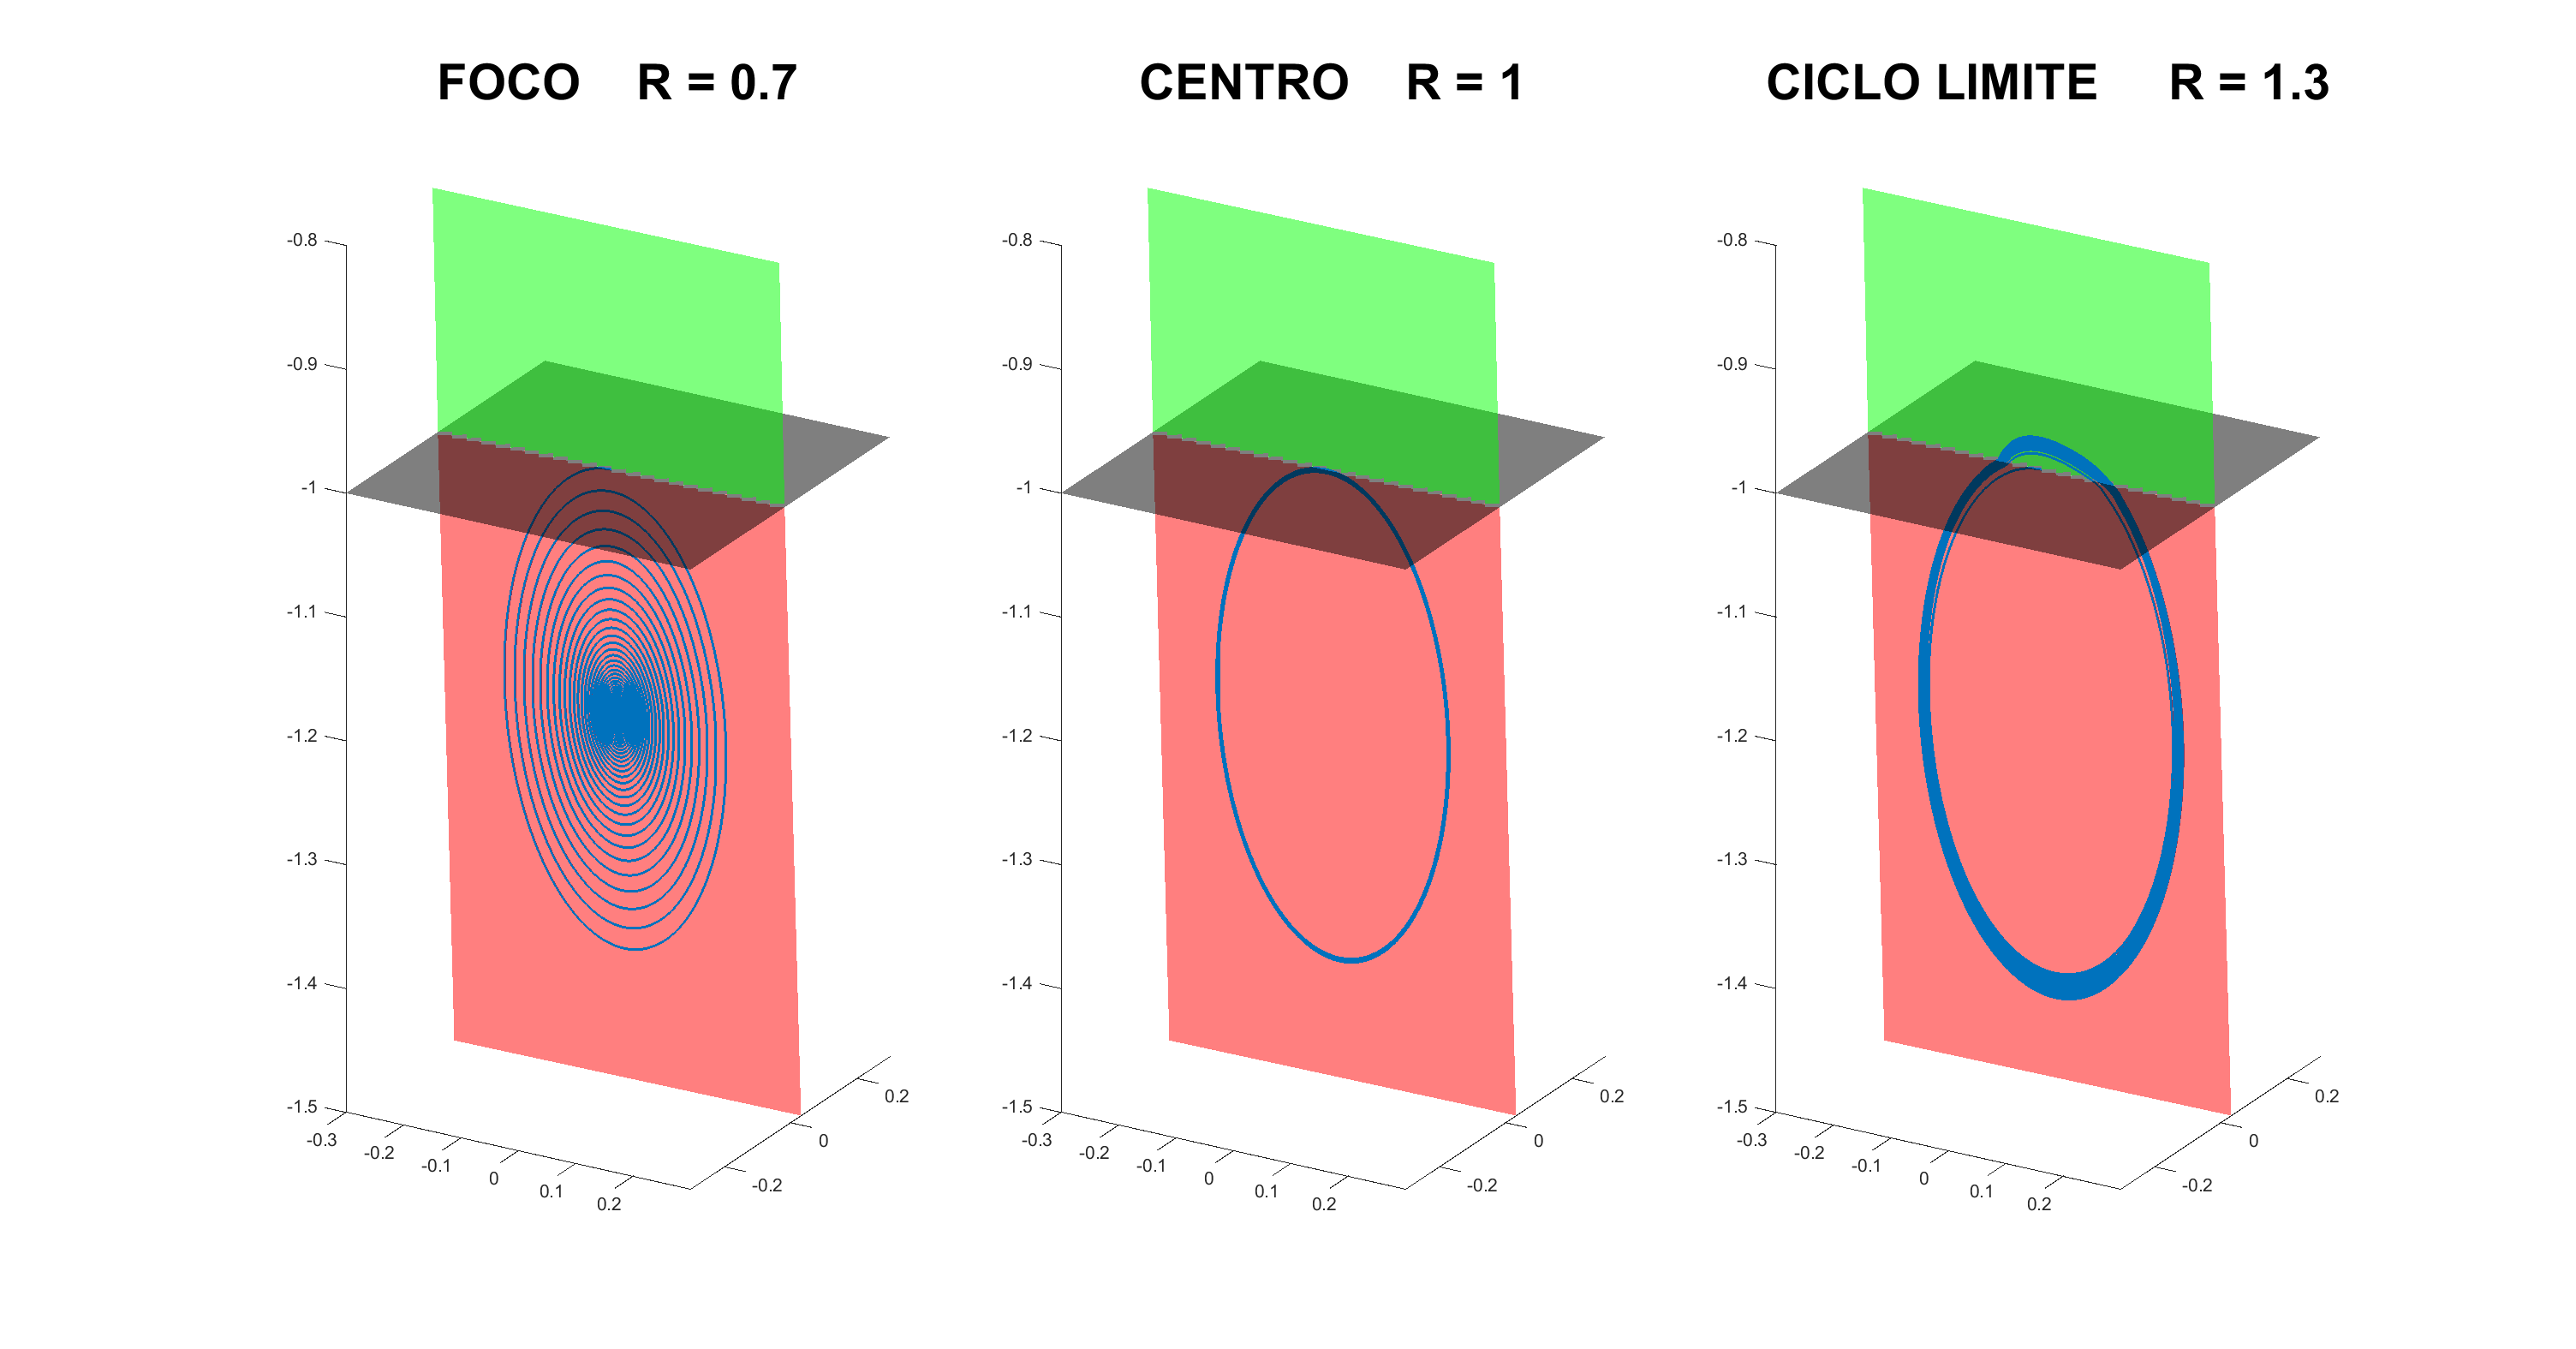
\includegraphics[width=1.3\textwidth,center]{3planoscircuito.eps}
		\caption{Gráfica resultado de ``Bifurcacion Combinar Planos''.}
		\label{fig:3planoscircuito}
	\end{figure}\smallskip
	
	\vspace{0.5cm} Como se puede comprobar en la \fref{fig:3planoscircuito}, efectivamente los planos rojo y verde pueden parecer el mismo, pero ya se ha demostrado en la \fref{fig:planoscircuito} que no es así.
	
	\newpage
	
	\chapter*{Conclusiones}
	
	En el transcurso de este trabajo, hemos explorado a fondo el potencial y la dinámica de este circuito oscilador construido con componentes electrónicos innovadores, y hemos aplicado rigurosamente conceptos teóricos clave. A través de nuestro análisis, hemos alcanzado valiosas conclusiones que arrojan luz sobre las posibilidades y limitaciones de este sistema, abriendo así la puerta a futuras investigaciones y aplicaciones en el campo de la electrónica y la utilización del Memristor. A lo largo de este estudio, hemos aplicado una gran cantidad de conceptos matemáticos de alto nivel y hemos logrado abstraernos del circuito para trabajar únicamente con expresiones matemáticas, obtener resultados en ellas y, finalmente, volver al circuito para corroborar que nuestros resultados son correctos.
	
	\vspace{0.5cm} Esta memoria ha sido la primera en utilizar la caracterización integral de la semiaplicación de Poincaré fuera del contexto puramente matemático, y esperamos que sirva como guía para que el resto de la comunidad científica se decida a utilizarla como una herramienta matemática de gran utilidad. Aspiramos a que este no sea más que el primero de muchos trabajos que la aprovechen.
	
	\vspace{0.5cm} Hemos demostrado que, a través de la aplicación rigurosa de conceptos matemáticos avanzados, es posible obtener una comprensión profunda de sistemas complejos como el que hemos estudiado, sin poner en riesgo la integridad del circuito mediante experimentación.
	
	\vspace{0.5cm} En última instancia, el futuro de la investigación científica en este ámbito es prometedor, y estamos ansiosos por presenciar los descubrimientos y avances que se avecinan. Esperamos que este trabajo contribuya al desarrollo de tecnologías innovadoras y al enriquecimiento de nuestro conocimiento sobre sistemas dinámicos y electrónicos.
	
	\addcontentsline{toc}{chapter}{Conclusiones}
	
	\newpage
	

	\begin{thebibliography}{99}
		\bibitem{chuamissing1971} CHUA, Leon O. ``Memristor – The missing circuit element.'' En: \textit{IEEE Transactions on Circuit Theory}, 1971, vol. CT-18, no. 5, pp. 507-519. \\DOI: \href{https://doi.org/10.1109/TCT.1971.1083337}{https://doi.org/10.1109/TCT.1971.1083337}
		
		\bibitem{chuaoscillator2008} ITOH, Makoto., CHUA, Leon O. ``Memristor Oscillators'' En: \textit{International Journal of Bifurcation and Chaos}, 2008, vol. 18, No. 11, pp. 3183-3206. \\DOI: \href{https://doi.org/10.1142/S0218127408022354}{https://doi.org/10.1142/S0218127408022354}
		
		\bibitem{HP} STRUKOV, D. B., SNIDER, G. S., STEWART, D. R., WILLIAMS, R. S. ``The missing memristor found'' En: \textit{Nature}, 2008, vol. 453(7191), pp. 80-3. \\DOI: \href{https://doi.org/10.1038/nature06932}{https://doi.org/10.1038/nature06932}
	
		\bibitem{williams} WILLIAMS, R. S. ``How We Found The Missing Memristor'' En: \textit{IEEE Spectrum}, 2008, vol. 45, no. 12, pp. 28-35, \\DOI: \href{https://doi.org/10.1109/MSPEC.2008.4687366}{https://doi.org/10.1109/MSPEC.2008.4687366}
		
		\bibitem{2021} Ji, Xiaoyue and Dong, Zhekang and Zhou, Guangdong and Lai, Chun Sing and Yan, Yunfeng and Qi, Donglian ``Memristive System Based Image Processing Technology: A Review and Perspective'' En: \textit{Electronics}, 2021, vol. 10, no. 24, p. 3176. \\DOI: \href{https://doi.org/10.3390/electronics10243176}{https://doi.org/10.3390/electronics10243176}
		
		\bibitem{outsiders} CARAVELLI, F., CARBAJAL, J. ``Memristors for the Curious Outsiders'' En: \textit{Technologies}, 2018, vol. 6, no. 4, p.118. \\DOI: \href{https://doi.org/10.3390/technologies6040118}{https://doi.org/10.3390/technologies6040118}
		
		\bibitem{teruel} LLIBRE, J., TERUEL, A. E. \textit{Introduction to the Qualitative Theory of Differential Systems}, Enero de 2014. Editorial: Springer Basel. eBook ISBN: 978-3-0348-0657-2. Hardcover ISBN: 978-3-0348-0656-5. \\DOI: \href{https://doi.org/10.1007/978-3-0348-0657-2}{https://doi.org/10.1007/978-3-0348-0657-2}
		
		\bibitem{docvic} CARMONA, V. ``Bifurcaciones en Sistemas Dinámicos Lineales a Trozos''. Tesis Doctoral. Universisdad de Sevilla, 2002. \\URL: \href{https://idus.us.es/handle/11441/15911?locale-attribute=en}{https://idus.us.es/handle/11441/15911}
		
		\bibitem{onsimplyfing} CARMONA, V., FREIRE, E., PONCE, E., TORRES, F. ``On simplifying and classifying piecewise-linear systems'' En: \textit{IEEE Transactions on Circuits and Systems I: Fundamental Theory and Applications}, 2002, vol. 49, no. 5, pp. 609-620. \\DOI: \href{https://doi.org/10.1109/TCSI.2002.1001950}{https://doi.org/10.1109/TCSI.2002.1001950}
		
		\bibitem{ponce} AMADOR, A., FREIRE, E., PONCE, E., ROS, J. ``On Discontinuous Piecewise Linear Models for Memristor Oscillators'' En: \textit{International Journal of Bifurcation and Chaos}, 2017, vol. 27, no. 6. \\DOI: \href{https://doi.org/10.1142/S0218127417300221
		}{https://doi.org/10.1142/S0218127417300221}
		
		\addcontentsline{toc}{chapter}{Bibliografía}
		\newpage
		
		
		\bibitem{properties}CARMONA, V., FERNÁNDEZ-SÁNCHEZ, F., GARCÍA-MEDINA, E., NOVAES, D. D. ``Properties of Poincaré half-maps for planar linear systems and some direct applications to periodic orbits of piecewise systems	'' En: \textit{Electron. J. Qual. Theory Differ. Equ.}, 2023, No. 22, 1-18, \\DOI: \href{https://doi.org/10.14232/ejqtde.2023.1.22}{https://doi.org/10.14232/ejqtde.2023.1.22}
		
		\bibitem{unicidad} CARMONA, V., FERNÁNDEZ-SÁNCHEZ, F., NOVAES, D. D. 
		``Uniqueness and stability of limit cycles in planar piecewise linear differential systems without sliding region'' En:
		\textit{Communications in Nonlinear Science and Numerical Simulation}, 2023, vol. 123, pp. 107257, ISSN 1007-5704,
		\\DOI: \href{https://doi.org/10.1016/j.cnsns.2023.107257}{https://doi.org/10.1016/j.cnsns.2023.107257}
		
		\bibitem{caracterizacion} CARMONA, V., FERNÁNDEZ-SÁNCHEZ, F.
		``Integral characterization for Poincaré half-maps in planar linear systems'' En: \textit{Journal of Differential Equations}, 2021, vol. 305, pp. 319-346, ISSN 0022-0396, \\DOI: \href{https://doi.org/10.1016/j.jde.2021.10.010}{https://doi.org/10.1016/j.jde.2021.10.010}
		
		\bibitem{ciclolimite} PONCE, E., ROS, J., VELA, E. \textit{The Focus-Center-Limit Cycle Bifurcation in Discontinuous Planar Piecewise Linear Systems Without Sliding}. Julio de 2013. Editorial: Springer, Berlin, Heidelberg. Print ISBN: 978-3-642-38829-3. Online ISBN: 978-3-642-38830-9. \\DOI: \href{https://doi.org/10.1007/978-3-642-38830-9_21}{https://doi.org/10.1007/978-3-642-38830-9\_21}
		
		\bibitem{amarillo} PONCE, E., ROS, J., VELA, E. \textit{Bifurcations in Continuous Piecewise Linear Differential Systems: Applications to Low-Dimensional Electronic Oscillators}. Diciembre de 2022. Editorial: Springer Cham. eBook ISBN: 978-3-031-21135-5. Hardcover ISBN: 978-3-031-21134-8. Softcover ISBN: 978-3-031-21137-9. \\DOI: \href{https://doi.org/10.1007/978-3-031-21135-5}{https://doi.org/10.1007/978-3-031-21135-5}
		
		\bibitem{pv} BACHMANN, K. H. ``Henrici, P., Applied and Computational Complex Analysis, Bd. I, 682 S., New York‐London‐Sydney‐Toronto. John Wiley \& sons. 1974. £ 13,50'' En: \textit{Zamm-zeitschrift Fur Angewandte Mathematik Und Mechanik}, 1977, vol. 57, pp.352-352. \\DOI: \href{ https://doi.org/10.1002/zamm.19770570622}{ https://doi.org/10.1002/zamm.19770570622}
		
		\bibitem{biolek} BIOLEK, Z., BIOLEK, D., BIOLKOVA, V. ``SPICE Model of Memristor with Nonlinear Dopant Drift'' En: \textit{Radioengineering}, 2009, vol. 18, no. 2, pp. 210-214 \\URL: \href{https://api.semanticscholar.org/CorpusID:19016545}{https://api.semanticscholar.org/CorpusID:19016545}
		
		\bibitem{perko} PERKO, L. \textit{Differential Equations and Dynamical Systems}, Diciembre del 2000. Editorial: Springer New York. eBook ISBN: 978-1-4613-0003-8. Hardcover ISBN: 978-0-387-95116-4. \\DOI: \href{https://doi.org/10.1007/978-1-4613-0003-8}{https://doi.org/10.1007/978-1-4613-0003-8}
		
		\bibitem{hirsch} HIRSCH, M. W., SMALE, S. \textit{Ecuaciones diferenciales, sistemas dinámicos y álgebra lineal}, 1983. Editorial: Alianza. ISBN 13: 9788420680613.
		
		\bibitem{simmons} SIMMONS, G. F. \textit{Ecuaciones diferenciales con aplicaciones y notas históricas}, Octubre de 1985. Editorial: McGraw-Hill. ISBN 13: 978-8476150696.
		
		\bibitem{zill} ZILL, D. \textit{Ecuaciones diferenciales con aplicaciones de modelado}, Julio de 2009. Editorial: Cengage Learning Editores S.A. de C.V. ISBN 13: 978-9708300551.
		
		\newpage
		
		\bibitem{clevermoller} MOLER, C. B. \textit{Numerical Computing with MATLAB }, Enero de 2004. Editorial: Society for Industrial and Applied Mathematics. ISBN 13: 978-0898715606.
		
		\bibitem{phaseplane} App ``\textit{Phase Plane and Slope Field}''
		\\URL:\hspace{1mm}\href{https://es.mathworks.com/matlabcentral/fileexchange/91705-phase-plane-and-slope-field-apps/}{https://es.mathworks.com/matlabcentral/fileexchange/91705-phase-plane-and-slope-field-apps/}
		
		\bibitem{tf1} APOSTOL, T. M. \textit{Análisis Matemático}, Enero de 1976. Editorial: Reverté. Segunda edición. ISBN: 978-84-291-5004-9.
		
	\end{thebibliography}
	
\end{document}
